%\documentclass[12pt,a4paper,twoside,openright]{amsbook} %{scrreprt}
%\usepackage{fancyhdr}
%\pagestyle{fancy}
%\newcommand{\subsubsubsection}{\paragraph}
   %%%%%%%%%%%%%%%%%%%%%%%%%%%%%%%%%%%%%%%%%%%%%%%%%%%%%%%%%%%%%%%%%%%%%%%%%%%%%%%
    %%% Layout %%%%%%%%%%%%%%%%%%%%%%%%%%%%%%%%%%%%%%%%%%%%%%%%%%%%%%%%%%%%%%%%%%%%%
    %%%%%%%%%%%%%%%%%%%%%%%%%%%%%%%%%%%%%%%%%%%%%%%%%%%%%%%%%%%%%%%%%%%%%%%%%%%%%%%%
\RequirePackage{fix-cm}

% default stuff that need to always be defined can be specifically overwritten by layouts

\newcommand{\listofinclusions}{
	
\phantomsection
	\addcontentsline{toc}{chapter}{Bildverzeichnis}
	\listoffigures
	\cleardoublepage

\phantomsection
	\addcontentsline{toc}{chapter}{Tabellenverzeichnis}
	\listoftables
	\cleardoublepage

\phantomsection
	\addcontentsline{toc}{chapter}{Algorithmenverzeichnis}
	\listofalgorithms
	\cleardoublepage
}

% ------------------------------------------------------------------------
%	Die KOMA-Script Dokumentklasse 'scrreprt' verwenden.
% http://www.dml.drzoom.ch/
% ------------------------------------------------------------------------
\documentclass[	pdftex, 
								a4paper,
								11pt, DIV11, BCOR5mm,
								parskip,								
								%draft,										
								%chapterprefix,					% entfernen	
								%pointlessnumbers					
								]{scrbook}
%
\makeatletter %%%%%%%%%%%%%%%%%%%%				% @ zu einem TeX-Zeichen machen
%
% ------------------------------------------------------------------------
%	Seitenlayout
% ------------------------------------------------------------------------
%\usepackage{setspace}
%\onehalfspace        										
%
\setcounter{secnumdepth}{4} 
\setcounter{tocdepth}{1}
%
\clubpenalty = 10000
\widowpenalty = 10000
\displaywidowpenalty = 10000
\usepackage{url}
\usepackage{amsmath}
%\usepackage{amssymb}
%\usepackage{amsfonts} 	

								
\usepackage{bbm}
% ------------------------------------------------------------------------
%	Schrift von serifenloser in Schrift *mit* Serifen ndern
% ------------------------------------------------------------------------
% alle auf einmal
%\setkomafont{sectioning}{\normalfont\bfseries}
%
%	Oder detailierter
%



%\setkomafont{chapter}{\normalfont\bfseries\sffamily\huge\color{chaptercolor}}				% fr Chapter
%\setkomafont{section}{\normalfont\bfseries\Large\color{chaptercolor}}			% fr Section
%\setkomafont{subsection}{\normalfont\bfseries\large\color{chaptercolor}}		% fr Subsection
%\setkomafont{subsubsection}{\normalfont\bfseries\color{chaptercolor}}			% fr SubSubSection
%\setkomafont{paragraph}{\normalfont\bfseries}					% fr Paragraph
%\setkomafont{subparagraph}{\normalfont\bfseries}				% fr SubParagraph
%\setkomafont{captionlabel}{\normalfont\bfseries\small} % fr Caption (Bildunterschrift usw.)
%


%\usepackage{times}

% ------------------------------------------------------------------------
%	Einstellen der deutschen Sprache, Verwendung von Umlauten, etc.
% ------------------------------------------------------------------------
%\usepackage[ngerman]{babel}							% neue deutsche Rechtschreibung
\usepackage[utf8]{inputenc}						% Eingabe von Umlauten ermglichen
%\usepackage[T1]{fontenc}								% Auswahl der Schrift
%\usepackage{ae}
\nonfrenchspacing 											% Nach Satzende groesserer Abstand
%
% ------------------------------------------------------------------------
%	Kopfzeilen
% http://www.physik.tu-berlin.de/pcpool/phcd/Dokumentation/LatexDoku/Proseminar/V07-footnote.pdf
% ftp://ftp.ctan.org/tex-archive/macros/latex/contrib/koma-script/scrguide.pdf (nach chaptermarkformat suchen)
% ------------------------------------------------------------------------
% 
\usepackage[automark,headsepline,headinclude]{scrpage2}

            
	% Kapitelnummer vor Kapiteltitel stellen
%\renewcommand*{\chaptermarkformat}{}			% nur Kapitel ohne 'Kapitel' oder Nummer anzeigen
%\renewcommand*{\sectionmarkformat}{}			% nur Section ohne Nummer anzeigen


\pagestyle{scrheadings}
\clearscrheadings													% Voreinstellugnen lschen
\clearscrplain														% Voreinstellugnen lschen
%\ohead{\leftmark\ -\ \rightmark}				% oben links: 'Kapitel - Section'
\ihead{\leftmark}													% oben links: 'Kapitel'
\ohead{\thepage}												% oben rechts aktuelle Seite
%\cfoot{\thepage}													
\setheadsepline{.4pt} 										% Linie unter der Kopfzeile
%\setfootsepline{.4pt}
\setlength{\headheight}{1.1\baselineskip}	% bei 1,5-fachem Zeilenabstand

%
% ------------------------------------------------------------------------
%	Glossar
% http://mrunix.de/forums/showthread.php?t=39944
%	http://www.dante.de/CTAN/macros/latex/contrib/nomencl/nomencl.pdf
% ------------------------------------------------------------------------
%
%\usepackage[german]{nomencl}							% nomenclature Glossar verwenden
%\usepackage{nomencl}
%\renewcommand{\nomname}{Glossary}					% Symbolverzeichnis in Glossar umbenennen
%\setlength{\nomlabelwidth}{.25\hsize}			% Breite des Begriffs (hier: 25% der Gesamtbreite)
%\renewcommand{\nomlabel}[1]{#1 \dotfill}	% Abstand zwischen Begriff und Beschreibung mit Punkten fllen
%\setlength{\nomitemsep}{-\parsep}					% Abstand der Linien zueinander
%
%\makenomenclature													% Glossar erzeugen
%\newglossaryentry{fotoreal}
{
  name=Fotorealistisches Rendering,
  description={bullshit}
}
\newglossaryentry{gameengine}
{
  name=Game Engine,
  plural = {Game Engines},
  description={Komplexes und mächtiges Softwarepakt für die Erstellung und Entwicklung von Videospielen, sowie deren Ausführung.}
}
\newglossaryentry{framework}
{
  name=Framework,
  description={Stellt einen domänenspezifisches Programmiergerüst für die Anwendungsentwicklung zur Verfügung. Neben der Softwarearchitektur kann das auch den Kontrollfluss und Schnittstellen einschließen.}
}
\newglossaryentry{mn}
{
  name = {Markov Netzwerk},
  description={Eine ungerichtete Graphstruktur, die eine Wahrscheinlichkeitsverteilung von komplexen Zusammenhängen von Zufallsvariablen modelliert.}
}
\newacronym{engine}{Engine}{als Kurzform von Unreal Engine verwendet}
\newacronym{ros}{\textsc{ROS}}{\textsc{Robot Operating System}}
\newacronym{vfh}{VFH}{Viewpoint Feature Histogram}
\newacronym{cnn}{CNN}{Convolutional Neural Network}
\newacronym{iai}{IAI}{Institute for Artificial Intelligence}
\newacronym[plural={SofAs}]{sofa}{SofA}{Subject of Analysis}
\newacronym{cas}{CAS}{Common Analysis Structure}
\newacronym[plural={AEs},longplural={Analysis Engines}]{ae}{AE}{Analysis Engine}
\newacronym{rf}{RF}{Random Forest}
\newacronym{svm}{SVM}{Support Vector Machine}
\newacronym{knn}{KNN}{K-Nearest Neighbour}
\newacronym{bson}{BSON}{Binary JSON}
\newacronym{sql}{SQL}{Structured Query Language}
\newacronym{rgb}{RGB}{Rot-Grün-Blau}
\newacronym[plural={MLNs},longplural={Markov Logic Networks}]{mln}{MLN}{Markov Logic Network}
\newacronym{fo}{FO}{Prädikatenlogik erster Stufe}
\newacronym[plural={PGMs},longplural={Probabilistischen Graphischen Modellen}]{pgm}{PGM}{Probabilistische Graphische Modelle}
\newacronym[plural={KBs},longplural={Wissensbasen}]{kb}{KB}{Wissensbasis}									% Glossareintrge aus extra Datei lesen
%
% ------------------------------------------------------------------------
%	Literaturverzeichnis
% ------------------------------------------------------------------------
%
%\usepackage{bibgerm}											% deutsche Anpassungen ans Literaturverzeichnis
%
%
% ------------------------------------------------------------------------
%	Stichwortverzeichnis
% http://www2.informatik.hu-berlin.de/~goerlach/Indexerstellung.pdf
% ------------------------------------------------------------------------
%
%\usepackage{makeidx}
%\makeindex																% Stichwortverzeichnis erzeugen
%
% ------------------------------------------------------------------------
%	PDF-Einstellungen
% http://www.math.uni-hamburg.de/home/iffland/Materialien/Einf_hyperref.pdf
% ------------------------------------------------------------------------

%\usepackage{lmodern}
\usepackage[pdfpagelabels,
						bookmarksopen,
						pdfstartview={FitV},
						plainpages=false,
						breaklinks=true,
						linkbordercolor={1 1 1},
						citebordercolor={1 1 1},
						urlbordercolor={1 1 1}]{hyperref}  % Stellt Verlinkungen im Dokument her
% Beim mehrmaligen vergeben von Seitenummern (rmisch,arabisch) gibt es gelegentlich
% Warnungen. Diese knnen aber ignoriert werden. siehe hierzu: 
% http://www.tex.ac.uk/cgi-bin/texfaq2html?label=hyperdupdest
%


% ------------------------------------------------------------------------
%	Grafics
% ------------------------------------------------------------------------
%\usepackage{graphicx}
%\usepackage[rm,bf,it,RM,IT]{subfigure}
\usepackage[usenames,dvipsnames]{color}
\definecolor{mblue}{gray}{0.5} % For some reason, this color is needed for sections			
%
% ------------------------------------------------------------------------
%	extended Tables
% ------------------------------------------------------------------------
%\usepackage{tabularx}
%\usepackage{booktabs}
%\usepackage{multirow}
%\usepackage{multicol}
%
% ------------------------------------------------------------------------
%	Font Settings
%  Available: Font Styles: cmr, guc; phv , pbk, pzc, ptm, ppl, pag
% ------------------------------------------------------------------------
% nonfree: ul9, ulg, ual
%\usepackage{kpfonts}
%\usepackage{lmodern}
%\usepackage{times}
%\usepackage{iwona}
%\usepackage{arev}
%\usepackage{cmbright}
\usepackage[charter]{mathdesign}
%\renewcommand{\sfdefault}{cmbr} %fvs
%\renewcommand{\rmdefault}{cmr}%{ppl}


\definecolor{chaptercolor}{rgb}{0,.639,.827}
\definecolor{sectioncolor}{rgb}{0,.639,.827}
%\definecolor{chapterbar}{rgb}{.56,.8,.56}%{.4,.639,.827}
\definecolor{chapterbar}{rgb}{.84,.09,.23}%AI Color

%\addtokomafont{chapter}{\usefont{T1}{fav}{b}{it}\color{black}}
\addtokomafont{section}{\usefont{T1}{fav}{b}{}\color{black}}
\addtokomafont{subsection}{\usefont{T1}{fav}{b}{}\color{black}}
\addtokomafont{subsubsection}{\usefont{T1}{fav}{b}{}\color{black}}

\addtokomafont{captionlabel}{\usefont{T1}{ppl}{b}{it}}%lmss
\addtokomafont{caption}{\usefont{T1}{ppl}{m}{it}}

\addtokomafont{sectioning}{\usefont{T1}{fav}{b}{it}}

\renewcommand{\headfont}{\usefont{T1}{lmss}{m}{it}}%uop

\usepackage{titlesec,lipsum}
\usepackage[table]{xcolor}
\automark[section]{chapter}

\setlength{\unitlength}{1cm}
\titleformat{\chapter}[display]
    { \usefont{T1}{fav}{b}{it}}
    { \hspace{1.5cm} \large{\chaptertitlename} \thechapter} 
    { .1pc }
    { \begin{picture}(10,0)(0,0)\color{chapterbar}\linethickness{.25cm}\put(.5,-.3){\line(0,1){2}} \hspace{1.5cm} \color{black}\Huge\usefont{T1}{fav}{b}{}}
    [ \end{picture} ]

%\usepackage{shadethm}

%\newshadetheorem{thms}{Theorem}[chapter]

%\newenvironment{thm}[1][]{%
%  \definecolor{shadethmcolor}{rgb}{.929,.968,.992}%
 % \definecolor{shaderulecolor}{rgb}{0.0,0.0,0.4}%
 % \setlength{\shadeboxrule}{1.5pt}%
%  \usefont{T1}{lmss}{m}{it}
%  \begin{thms}[#1]\hspace*{1mm}%
%}{\end{thms}}


%
% ------------------------------------------------------------------------
%	Erweiterung um MetaPost-Dateien direkt einzubinden.
% ------------------------------------------------------------------------
%\makeatletter
%\@ifundefined{pdfoutput}{}{\DeclareGraphicsRule{*}{mps}{*}{}}
%\makeatother
%
% ------------------------------------------------------------------------
%	Fu�zeilen in \caption einer float Umgebung verwenden.
% http://www.tex.ac.uk/tex-archive/macros/latex/contrib/ccaption/ccaption.pdf
% ------------------------------------------------------------------------
\usepackage[caption2]{ccaption}
\usepackage{dsfont}

\newenvironment{items}{\begin{itemize}\setlength{\itemsep}{-5mm} \setlength{\topsep}{-10mm} \setlength{\parsep}{20mm}}{\end{itemize}} 

\newenvironment{enum}{\begin{enumerate}\setlength{\itemsep}{-5mm} \setlength{\topsep}{-5mm} \setlength{\parsep}{-5mm}}{\end{enumerate}}

%%%%%%%%%%%%%%%%%%%%%%%%%%%%%%%%%%%%%%%%%%%%%%%%%%%%%%%%%%%%%%%%%%%%%%%%%%%%%%%%
%%% Include Packages %%%%%%%%%%%%%%%%%%%%%%%%%%%%%%%%%%%%%%%%%%%%%%%%%%%%%%%%%%%
%%%%%%%%%%%%%%%%%%%%%%%%%%%%%%%%%%%%%%%%%%%%%%%%%%%%%%%%%%%%%%%%%%%%%%%%%%%%%%%%

\usepackage[toc,acronym]{glossaries}
\usepackage[british,english,ngerman]{babel}
\usepackage[section]{placeins}
\usepackage{epstopdf}
\usepackage{textpos}
%\usepackage{comment}
%\usepackage{etex}
\usepackage{changepage}
%\usepackage{epsfig}
\usepackage{theorem}
%\usepackage{amsthm}
%\usepackage{float}
\usepackage{caption}
%\usepackage[style=german,threshold=1,german=quotes]{csquotes}
\usepackage{subcaption}
\usepackage[T1]{fontenc}
%\usepackage{framed}
%\usepackage{graphics}
\usepackage{graphicx}
%\usepackage[table]{xcolor}
%\usepackage{iasbib} % use the IAS bibliography files (needs iasdocs repository)
%\usepackage{ifthen}
%\usepackage[intoc,noprefix]{nomencl} % for list of symbols, notations
\usepackage{listings}
%\usepackage{longtable} \usepackage{makeidx}
%\usepackage{multicol}
%\usepackage{multirow}
%\usepackage[round,comma,colon,authoryear]{natbib}
\usepackage[square,comma,numbers,sort]{natbib}
%\usepackage{setspace}
%\usepackage[format=hang]{subfig} % format=hang
%\usepackage{times}
%usepackage{units}
%\usepackage{upgreek}
%\usepackage{url}
\usepackage{tabularx}
\usepackage{booktabs}
%\usepackage{texinclude/mysects}
%\usepackage{texinclude/tumlogo}
%\usepackage{texinclude/tumabakus}
\usepackage{tikz}
\usetikzlibrary{decorations.markings,arrows,positioning,trees,calc,fit,shapes}
\usepackage{varwidth}
%\usepackage{tikz}
%\usepackage{wrapfig}
\usepackage{xspace}
%\usepackage{import}
%\usepackage{enumerate}
%\usepackage{colonequals}
%\usepackage{eso-pic}
\usepackage[ruled, linesnumbered]{algorithm2e}
%\usepackage[noend]{algorithmic}
%\usepackage{algorithm}
%\usepackage{cancel}
%\usepackage{multimedia}
%\usepackage{iaspresentationdefs}
%\usepackage[chapter]{algorithm}
%\usepackage[noend]{algorithmic}
\usepackage{environ}
%\usepackage{colortbl}
%\usepackage[pdftex]{hyperref}
\usepackage[utf8]{inputenc}
%\usepackage{bbm} % enables \mathbbm as a perhaps nicer alternative version of \mathbb
%\usepackage{tweaklist}
%\usepackage{pbox}
%\usepackage{varwidth}
%\usepackage[leftcaption]{sidecap}
%\usepackage{bibentry}
%\usepackage{blindtext}

\usetikzlibrary{decorations}

	% BIBLIOGRAPHY SETTINGS
\bibliographystyle{alphadin}

%\newcommand{\todo}[1]{\textcolor{red}{\textbf{TODO}: #1}}
%%%%%%%%%%%%%%%%%%%%%%%%%%%%%%%%%%%%%%%%%%%%%%%%%%%%%%%%%%%%%%%%%%%%%%%%%%%%%%%%
%%%                  %%%%%%%%%%%%%%%%%%%%%%%%%%%%%%%%%%%%%%%%%%%%%%%%%%%%%%%%%%%
%%%%%%%%%%%%%%%%%%%%%%%%%%%%%%%%%%%%%%%%%%%%%%%%%%%%%%%%%%%%%%%%%%%%%%%%%%%%%%%%

\frenchspacing
\newglossary[slg]{symbolslist}{syi}{syg}{Symbols}
\renewcommand*{\glspostdescription}{}
\makeglossaries
\makeindex
%\makenomenclature       % helps build the list of symbols/notes
\renewcommand*{\glossaryentrynumbers}[1]{}


\NewEnviron{centerbox}[1][\linewidth]{% \begin{centerbox}[..] ... \end{centerbox}
  \noindent\makebox[\linewidth][c]{%
    \begin{minipage}{#1}%
      \raggedright% Minipage alignment
      \BODY% Typeset body/contents
    \end{minipage}%
  }
}

\NewEnviron{texto}{%
    \begin{center}
        \begin{varwidth}[t]{\textwidth}

        \raggedright
        \BODY
        \end{varwidth}
    \end{center}
}


\graphicspath{./img}
%%%%%%%%%%%%%%%%%%%%Declare tikz external images%%%%%%%%%%%%%%%%%%%%%%%%%%%%%%%
%\pgfdeclareimage{cheese}{cheese.jpg}

%%%%%%%%%%%%%%%%%%%%%%%%%%%%%%%%%%%%%%%%%%%%%%%%%%%%%%%%%%%%%%%%%%%%%%%%%%%%%%%%
%%% Relevant Thesis Information %%%%%%%%%%%%%%%%%%%%%%%%%%%%%%%%%%%%%%%%%%%%%%%%
%%%%%%%%%%%%%%%%%%%%%%%%%%%%%%%%%%%%%%%%%%%%%%%%%%%%%%%%%%%%%%%%%%%%%%%%%%%%%%%%

%%%THESIS INFO
\newcommand{\firstreviewer}{Prof. Michael Beetz}
\newcommand{\secondreviewer}{Dr. René Weller}
\newcommand{\supervisor}{Ferenc Bálint-Benczédi}
\newcommand{\thesistype}{Bachelorarbeit}
\newcommand{\myauthor}{Dominik Dieckmann}
\newcommand{\mymaintitle}{Probabilistische Szenen-Interpretation mit Virtueller Realität und Markov-Logik-Netzwerken}
\newcommand{\mysubtitle}{Probabilistic Scene Understanding using Virtual Reality and Markov Logic Networks}
\newcommand{\mytitle}{\centering {\Huge \mymaintitle}\\[.3in] 
    {\Large \mysubtitle}}
\newcommand{\pdftitle}{\mymaintitle - \mysubtitle}
\newcommand{\formattedfronttitle}{{\mytitle}}
\newcommand{\formattedinnertitle}{{\mytitle}}





\newcommand{\dotrule}[1]{%
   \parbox[t]{#1}{\dotfill}}
\newcommand{\chairman}{\dotrule{7cm}}
%\newcommand{\firstreviewer}{\dotrule{7cm}}
%\newcommand{\secondreviewer}{\dotrule{7cm}}
%\newcommand{\thirdreviewer}{\dotrule{7cm}}
\newcommand{\handindate}{\dotrule{4cm}}
\newcommand{\acceptancedate}{\dotrule{4cm}}


\hypersetup{
  pdftitle={\pdftitle},
  pdfauthor={\myauthor},
  pdfcreator={\myauthor},
  pdfproducer={\myauthor}
}


%\pdfinfo { /Title \pdftitle           /Author \myauthor}
\theoremstyle{plain}
\newtheorem{definition}{Definition}[section]
\newtheorem{theorem}{Theorem}[section]
\newtheorem{assumption}{Assumption}[section]
\newtheorem{example}{Example}[section]
%%%%%%%%%%%%%%%%%%%%%%%%%%%%%%%%%%%%%%%%%%%%%%%%%%%%%%%%%%%%%%%%%%%%%%%%%%%%%%%%%
%%% User commands %%%%%%%%%%%%%%%%%%%%%%%%%%%%%%%%%%%%%%%%%%%%%%%%%%%%%%%%%%%%%%
%%%%%%%%%%%%%%%%%%%%%%%%%%%%%%%%%%%%%%%%%%%%%%%%%%%%%%%%%%%%%%%%%%%%%%%%%%%%%%%%

%\DeclareGraphicsExtensions{.pdf,.jpeg,.png,.jpg}
%\graphicspath{{./}{./bln/techrep/}{../../../pictures/src/probcog/AMLNs/}{../../../pictures/src/probcog/AMLNs/weightcurves/}{../../../pictures/src/probcog/MCSATPC/}{../../../pictures/bin/}{../../../pictures/src/}{../../../pictures/src/probcog/}{../../../../code/SRLDB/experiments/sampling/}}
\definecolor{backcolour}{rgb}{0.95,0.95,0.92}
\definecolor{lightgray}{gray}{0.85}
\setlength{\extrarowheight}{1pt}
%%%%%%%%%%%%%%%%%%%%%%%%%%%%%%%%%%%%%%%%%%%%%%%%%%%%%%%%%%%%%%%%%%%%%%%%%%%%%%%%
%%% User commands %%%%%%%%%%%%%%%%%%%%%%%%%%%%%%%%%%%%%%%%%%%%%%%%%%%%%%%%%%%%%%
%%%%%%%%%%%%%%%%%%%%%%%%%%%%%%%%%%%%%%%%%%%%%%%%%%%%%%%%%%%%%%%%%%%%%%%%%%%%%%%%

\newcommand{\subsubsubsection}{\paragraph}

\newcommand{\levela}{}
\newcommand{\levelb}{}
\newcommand{\levelc}{}
\newcommand{\leveld}{}
\newcommand{\levele}{}

\newcommand{\sublevela}{}
\newcommand{\sublevelb}{}
\newcommand{\sublevelc}{}

\newcommand{\todo}[1]{\textcolor{red}{\textbf{TODO}: #1}}

% *** regular text ***

\newcommand{\ie}{i.e.\xspace}
\newcommand{\eg}{e.g.\xspace}
\newcommand{\quot}[1]{``#1''\xspace}
\newcommand{\secs}{$\,$s}
\newcommand{\urlwofont}[1]{\urlstyle{same}\url{#1}}
\newcommand{\keyword}[1]{\emph{#1}\index{#1}\xspace}

\newcommand{\imgcopyright}[2][]{{\scriptsize{#1 \copyright~#2}}}
\newcommand{\imgnote}[1]{{\scriptsize{#1}}}

\newenvironment{itemize*}%
  {\begin{itemize}%
    \setlength{\itemsep}{0.5ex}%
    \setlength{\parskip}{0pt}}%
  {\end{itemize}}

\newenvironment{enumerate*}%
  {\begin{enumerate}%
    \setlength{\itemsep}{0.5ex}%
    \setlength{\parskip}{0pt}}%
  {\end{enumerate}}
 
\newenvironment{tabbing*}
   {\setlength{\topsep}{-\parskip}%
    \setlength{\partopsep}{0pt}%
    \tabbing}
   {\endtabbing}

\definecolor{shadecolor}{rgb}{0.92,0.92,0.92}
\newenvironment{pquery}
   {\hspace{1cm}\begin{minipage}{0.9\linewidth}\slshape\footnotesize\begin{shaded}\begin{tabbing*}}
   {\end{tabbing*}\end{shaded}\end{minipage}}
   
 \newcommand{\queryEmph}[1]{\textbf{#1}}

% *** general formula stuff

%\newcommand{\mw}[1]{\mathrm{\textsl{#1}}}
\newcommand{\mw}[1]{\mbox{\textsl{#1}}}
\newcommand{\mword}[1]{\mw{#1}}
%\newcommand{\argmax}{\operatornamewithlimits{arg\,max\,}}
\DeclareMathOperator*{\argmax}{arg\,max\,}

\newcommand{\wwedge}{\,\wedge\,}

% functions and constants
\newcommand{\Var}{\mathrm{Var}}
\newcommand{\dom}{\mathrm{dom}}
\newcommand{\cnt}{\mathrm{\textsl{count}}}
\newcommand{\true}{\mathrm{\textsl{True}}}
\newcommand{\false}{\mathrm{\textsl{False}}}
\newcommand{\True}{\true}
\newcommand{\False}{\false}
\newcommand{\pa}{\mathrm{par}}
\newcommand{\Pa}{\mathrm{Par}}
\newcommand{\hatF}{\hat{F}}
\newcommand{\hatf}{\hat{f}}
\newcommand{\hatw}{\hat{w}}
\newcommand{\hatlambda}{\hat{\lambda}}

\newcommand{\impl}{\Rightarrow}
\newcommand{\biimpl}{\Leftrightarrow}
\newcommand{\given}{\mid}
\newcommand{\deriv}[1]{\frac{\delta}{\delta #1}\,}
\renewcommand{\hat}{\widehat}
%\newcommand{\mod}{\ \mathrm{mod}\ }

% MLNs
\newcommand{\mrf}{M_{L,D}}
\newcommand{\bird}{\mw{bird}}
\newcommand{\flies}{\mw{flies}}
\newcommand{\veg}{\mw{vegetarian}}
\newcommand{\vegdish}{\mw{vegDish}}
\newcommand{\friends}{\mw{friends}}
\newcommand{\female}{\mw{female}}
\newcommand{\orders}{\mw{orders}}
\newcommand{\evar}{e}

% probability constraints
\newcommand{\probconstr}{\mathcal{R}_F}
\newcommand{\gndfpcf}{\hatF_{R_k}}

% uncertain evidence
\newcommand{\se}{{s_E}}

% confidence intervals
\newcommand{\smax}{s_\mathrm{max}}
\newcommand{\ubound}{p_u}
\newcommand{\lbound}{p_l}
\newcommand{\pmode}{\tilde{p}}

% *** names ***
\newcommand{\robosherlock}{\textsc{RoboSherlock}\xspace}
\newcommand{\robcog}{\textsc{RobCoG}\xspace}
\newcommand{\mongodb}{\textsc{MongoDB}\xspace}
\newcommand{\unreal}{\textsc{Unreal Engine}\xspace}
\newcommand{\pracmln}{\textsc{pracmln}\xspace}
\newcommand{\fuzzymln}{\textsc{Fuzzy-MLN}\xspace}

\newcommand{\probcog}{\textsc{ProbCog}\xspace}
\newcommand{\knowrob}{\textsc{KnowRob}\xspace}
\newcommand{\cram}{\textsc{CRAM}\xspace}
\newcommand{\cpl}{\textsc{CRAM-PL}\xspace}
\newcommand{\cogito}{\textsc{Cogito}\xspace}
\newcommand{\cotesys}{CoTeSys\xspace}
\newcommand{\kcopman}{\textsc{K-CoPMan}\xspace}
\newcommand{\rosie}{TUM-Rosie\xspace}
\newcommand{\james}{TUM-James\xspace}

% *** algorithm stuff ***

\newcommand{\IFTHEN}[2]{\STATE \algorithmicif\ #1\ \algorithmicthen\ {#2}}
\renewcommand{\listalgorithmname}{Algorithmenverzeichnis} % Renaming List of Algorithm 
% \algorithmicendif}

% *** listings and code snippets ***

\definecolor{randvarcolor}{HTML}{B1CBDA} % colour of random variables everywhere
\definecolor{darkrandvarcolor}{HTML}{004F9E} %{00476D} % darker, more saturated version of the former colour

\lstset{
	basicstyle=\sffamily\footnotesize,
	keywordstyle=\color{darkrandvarcolor}\bfseries,
	morekeywords={type,random,isa,logical,relationKey,prolog,fragments,constraints,guaranteed,combining,rule,uniform,default},
	numbers=left,
	xleftmargin=25pt,
	escapeinside={(@}{@)}
}

\lstnewenvironment{blnlisting}
{\lstset{
		basicstyle=\sffamily\footnotesize,
		keywordstyle=\color{darkrandvarcolor}\bfseries,
		morekeywords={type,random,isa,logical,relationKey,prolog,fragments,constraints,guaranteed,combining,rule,uniform,default},
		numbers=left,
		xleftmargin=25pt,
		breaklines=true,
		columns=fullflexible,
		escapeinside={(@}{@)}
		}}
{\vspace{-0.5\baselineskip}\ignorespacesafterend}

\newcommand{\inputbln}[1]{\lstinputlisting[
		basicstyle=\sffamily\scriptsize,
		keywordstyle=\color{darkrandvarcolor}\bfseries,
		morekeywords={type,random,isa,logical,relationKey,prolog,fragments,constraints,constraint,guaranteed,combining,rule,uniform,default},
		numbers=left,
		xleftmargin=25pt,
		breaklines=true,
		columns=fullflexible,
		escapeinside={(@}{@)}
]{#1}}

\newcommand{\blncode}[1]{{\small\textsf{#1}}}

\newenvironment{mln}[1][l]{

\vspace{1.5ex}

\hspace{0.7cm}\begin{minipage}{0.9\linewidth}\small
\begin{tabular}{l@{\hspace{2ex}}#1}}
{\end{tabular}\end{minipage}

\vspace{1.5ex}

\noindent}

\DeclareCaptionType[fileext=lomln,placement={!ht}]{mlnmodel}[MLN]
\DeclareCaptionType[fileext=lobln,placement={!ht}]{blnmodel}[BLN]
\newsubfloat{blnmodel} % enable subfloats in blnmodel env.

%%%%%%%%%%%%%%%%%%%%%%%%%%%%%%%%%%%%%%%%%%%%%%%%%%%%%%%%%%%%%%%%%%%%%%%%%%%%%%%
%%% Glossary %%%%%%%%%%%%%%%%%%%%%%%%%%%%%%%%%%%%%%%%%%%%%%%%%%%%%%%%%%%%%%%%%%%
%%%%%%%%%%%%%%%%%%%%%%%%%%%%%%%%%%%%%%%%%%%%%%%%%%%%%%%%%%%%%%%%%%%%%%%%%%%%%%%%
\newglossaryentry{fotoreal}
{
  name=Fotorealistisches Rendering,
  description={bullshit}
}
\newglossaryentry{gameengine}
{
  name=Game Engine,
  plural = {Game Engines},
  description={Komplexes und mächtiges Softwarepakt für die Erstellung und Entwicklung von Videospielen, sowie deren Ausführung.}
}
\newglossaryentry{framework}
{
  name=Framework,
  description={Stellt einen domänenspezifisches Programmiergerüst für die Anwendungsentwicklung zur Verfügung. Neben der Softwarearchitektur kann das auch den Kontrollfluss und Schnittstellen einschließen.}
}
\newglossaryentry{mn}
{
  name = {Markov Netzwerk},
  description={Eine ungerichtete Graphstruktur, die eine Wahrscheinlichkeitsverteilung von komplexen Zusammenhängen von Zufallsvariablen modelliert.}
}
\newacronym{engine}{Engine}{als Kurzform von Unreal Engine verwendet}
\newacronym{ros}{\textsc{ROS}}{\textsc{Robot Operating System}}
\newacronym{vfh}{VFH}{Viewpoint Feature Histogram}
\newacronym{cnn}{CNN}{Convolutional Neural Network}
\newacronym{iai}{IAI}{Institute for Artificial Intelligence}
\newacronym[plural={SofAs}]{sofa}{SofA}{Subject of Analysis}
\newacronym{cas}{CAS}{Common Analysis Structure}
\newacronym[plural={AEs},longplural={Analysis Engines}]{ae}{AE}{Analysis Engine}
\newacronym{rf}{RF}{Random Forest}
\newacronym{svm}{SVM}{Support Vector Machine}
\newacronym{knn}{KNN}{K-Nearest Neighbour}
\newacronym{bson}{BSON}{Binary JSON}
\newacronym{sql}{SQL}{Structured Query Language}
\newacronym{rgb}{RGB}{Rot-Grün-Blau}
\newacronym[plural={MLNs},longplural={Markov Logic Networks}]{mln}{MLN}{Markov Logic Network}
\newacronym{fo}{FO}{Prädikatenlogik erster Stufe}
\newacronym[plural={PGMs},longplural={Probabilistischen Graphischen Modellen}]{pgm}{PGM}{Probabilistische Graphische Modelle}
\newacronym[plural={KBs},longplural={Wissensbasen}]{kb}{KB}{Wissensbasis}

%%%%%%%%%%%%%%%%%%%%%%%%%%%%%%%%%%%%%%%%%%%%%%%%%%%%%%%%%%%%%%%%%%%%%%%%%%%%%%%%
%% Document start %%%%%%%%%%%%%%%%%%%%%%%%%%%%%%%%%%%%%%%%%%%%%%%%%%%%%%%%%%%%%
%%%%%%%%%%%%%%%%%%%%%%%%%%%%%%%%%%%%%%%%%%%%%%%%%%%%%%%%%%%%%%%%%%%%%%%%%%%%%%%%

\begin{document}
\lstset{language=C++}
\setcounter{page}{-2}
\pagestyle{empty}
\pagenumbering{none}

%\newglossaryentry{fotoreal}
{
  name=Fotorealistisches Rendering,
  description={bullshit}
}
\newglossaryentry{gameengine}
{
  name=Game Engine,
  plural = {Game Engines},
  description={Komplexes und mächtiges Softwarepakt für die Erstellung und Entwicklung von Videospielen, sowie deren Ausführung.}
}
\newglossaryentry{framework}
{
  name=Framework,
  description={Stellt einen domänenspezifisches Programmiergerüst für die Anwendungsentwicklung zur Verfügung. Neben der Softwarearchitektur kann das auch den Kontrollfluss und Schnittstellen einschließen.}
}
\newglossaryentry{mn}
{
  name = {Markov Netzwerk},
  description={Eine ungerichtete Graphstruktur, die eine Wahrscheinlichkeitsverteilung von komplexen Zusammenhängen von Zufallsvariablen modelliert.}
}
\newacronym{engine}{Engine}{als Kurzform von Unreal Engine verwendet}
\newacronym{ros}{\textsc{ROS}}{\textsc{Robot Operating System}}
\newacronym{vfh}{VFH}{Viewpoint Feature Histogram}
\newacronym{cnn}{CNN}{Convolutional Neural Network}
\newacronym{iai}{IAI}{Institute for Artificial Intelligence}
\newacronym[plural={SofAs}]{sofa}{SofA}{Subject of Analysis}
\newacronym{cas}{CAS}{Common Analysis Structure}
\newacronym[plural={AEs},longplural={Analysis Engines}]{ae}{AE}{Analysis Engine}
\newacronym{rf}{RF}{Random Forest}
\newacronym{svm}{SVM}{Support Vector Machine}
\newacronym{knn}{KNN}{K-Nearest Neighbour}
\newacronym{bson}{BSON}{Binary JSON}
\newacronym{sql}{SQL}{Structured Query Language}
\newacronym{rgb}{RGB}{Rot-Grün-Blau}
\newacronym[plural={MLNs},longplural={Markov Logic Networks}]{mln}{MLN}{Markov Logic Network}
\newacronym{fo}{FO}{Prädikatenlogik erster Stufe}
\newacronym[plural={PGMs},longplural={Probabilistischen Graphischen Modellen}]{pgm}{PGM}{Probabilistische Graphische Modelle}
\newacronym[plural={KBs},longplural={Wissensbasen}]{kb}{KB}{Wissensbasis}
\begin{titlepage}
	\vspace*{-2.2cm}
	\begin{adjustwidth}{-0cm}{-2.3cm}
	\thispagestyle{empty}
        \begin{figure}
            \begin{minipage}{.4\linewidth}
	\begin{flushleft}
		
\includegraphics[height=1.5cm]{unihb/unilogo-transp.pdf}
	
		%\lipsum[1-2]
	\end{flushleft}
    \end{minipage}
    \hspace{.2\linewidth}
            \begin{minipage}{.4\linewidth}
	\begin{flushright}
		
\includegraphics[height=3.0cm]{unihb/logo-ai-small.pdf}
	
		%\lipsum[1-2]
	\end{flushright}
    \end{minipage}
\end{figure}
	
	  \vfill
	  
	  \scalebox{0.95}{
	  \begin{minipage}{1.2\textwidth}
	  {
		\formattedfronttitle
	  }
	  \end{minipage}
	  }
	%\begin{center}
	  \vfill
	  
	  {\Large \thesistype}\\[2.5ex]
	  {\Large\em \myauthor}
	  
	  \vfill
	{  
      \renewcommand\arraystretch{1.5}
      \begin{tabular}{l@{\hspace{2em}}r@{\hspace{1ex}}p{7cm}}
        Pr\"ufer der \thesistype: & 1. & \firstreviewer\\
                                   & 2. & \secondreviewer\\
	Betreuer:		    &   & \supervisor\\
      \end{tabular}
  }
	%\end{center}
	\end{adjustwidth}
\setlength{\parskip}{1pt}
%\definecolor{cyan}{RGB}{88, 190, 184}
%\noindent \begin{flushright}
%\includegraphics[width=55mm,height=16mm]{tum/sts-titelblatt/pics/tuhh_logo}
%\par\end{flushright}
%
%\textcolor{cyan}{\rule[0.5ex]{1\columnwidth}{0.5pt}}
%
%\textsf{\textcolor{cyan}{\Large Master Thesis}}{\Large \par}
%
%\textcolor{cyan}{\rule[0.5ex]{1\columnwidth}{0.5pt}}
%
%\vspace{32mm}
%
%
%\noindent \begin{flushright}
%\textsf{\Large  Author N.N.}\textsf{\textbf{\Large }}\\
%\textsf{\vspace{1.2cm}
%}
%\par\end{flushright}
%
%\noindent \begin{flushright}
%	\formattedfronttitle
%%\textsf{\huge Working }\\
%%\textsf{\huge Title}
%\par\end{flushright}{\huge \par}
%
%\vspace{25mm}
%
%
%\noindent \begin{flushright}
%\textsf{\Large Date}
%\par\end{flushright}{\Large \par}
%
%\noindent \begin{flushleft}
%\textsf{\vspace{16mm}
%}\textcolor{cyan}{\rule[0.5ex]{1\columnwidth}{0.5pt}}\\
%\textsf{\textcolor{cyan}{\large supervised by:}}\textsf{}\\
%\textsf{Prof. Dr. N.N.}\\
%\textsf{Prof. Dr. N.N.}\textcolor{cyan}{}\\
%\textcolor{cyan}{\rule[0.5ex]{1\columnwidth}{0.5pt}\begin{textblock}{3}(12.7,0.2)\includegraphics[width=23mm,height=23mm]{tum/sts-titelblatt/pics/STS-Logo}\end{textblock}}\textsf{\textcolor{cyan}{Hamburg University of Technology (TUHH)}}\\
%\textsf{\textcolor{cyan}{\textit{Technische Universit{\"a}t Hamburg-Harburg}}}\\
%\textsf{\textcolor{cyan}{Institute for Software Systems}}\\
%%\textsf{\textcolor{cyan}{Schwarzenbergstr.~95}}\\
%\textsf{\textcolor{cyan}{21073 Hamburg}}
%\par\end{flushleft}
\end{titlepage}


\cleardoublepage

\pagestyle{headings}
%\include{title}
%\cleardoublepage
\pagenumbering{Roman}
\setcounter{page}{1}
\phantomsection
\addcontentsline{toc}{chapter}{Eidesstattliche Erkl\"arung}
\chapter*{Eidesstattliche Erkl\"arung}



Hiermit erkl\"are ich, dass ich die vorliegende Arbeit selbstst\"andig angefertigt,
nicht anderweitig zu Pr\"ufungszwecken vorgelegt und keine anderen als die
angegebenen Hilfsmittel verwendet habe. S\"amtliche wissentlich verwendete
Textausschnitte, Zitate oder Inhalte anderer Verfasser wurden ausdr\"ucklich als
solche gekennzeichnet.

Bremen, den \makeatletter\@date\makeatother

\vspace*{1em}
\rule{15em}{0.16667pt}\\
\myauthor
\makeatletter\@author\makeatother
\cleardoublepage

%\phantomsection
%\addcontentsline{toc}{chapter}{Acknowledgements}
%\chapter*{Acknowledgements}


Add your acknowledgements here don't forget your supervisor
%\cleardoublepage

\phantomsection
\addcontentsline{toc}{chapter}{Kurzfassung}
\chapter*{Kurzfassung} 

In Haushaltsumgebungen eingesetzte autonome Roboter müssen in der Lage sein, mit den durch den Menschen verursachten nichtdeterministischen Veränderungen, umgehen zu können. Für viele Aufgaben ist es vonnöten, Objekte wahrzunehmen und ihnen aus bekanntem Wissen eine Bedeutung zu geben. Als Grundlage dient dazu eine Perzeptionskomponente, mit der die Umgebungen wahrgenommen und durch Segmentierung Objekte gefunden werden können. Um die Objekte zu interpretieren, ihnen eine Bedeutung zu geben, wird über eine Wissensbasis geschlussfolgert. Wissensbasen müssen vorher jedoch mit Beispielen, den sogenannten Trainingsdaten, trainiert werden. Da die Wissensbasis für die Wahrnehmung verwendet wird, handelt es sich bei den Trainingsdaten um Bilder von möglichen wahrnehmbaren Szenen. Das Trainieren einer Wissensbasis ist jedoch mit hohem Aufwand verbunden, denn die Bilder müssen manuell erstellt werden und für komplexe Umgebungen sind in der Regel auch eine große Anzahl vonnöten. Diese Arbeit untersucht, ob der Aufwand verringert werden könnte, indem in einer Game Engine synthetisch erzeugte Bilder zum Training verwendet werden. Dazu werden in der \unreal fotorealistische Virtuelle Szenen erzeugt. Das Perzeptionsframework \robosherlock segmentiert diese und die gewonnenen Informationen werden verwendet, um eine Wissensbasis in Form eines Markov-Logik-Netzwerkes zu trainieren. Zur Evaluation wird die Güte der Objektklassifikation durch das MLN in wahrgenommenen Szenen untersucht. 

\cleardoublepage

%\addcontentsline{toc}{chapter}{Kurzfassung}
%\include{kurzfassung}
%\cleardoublepage


\phantomsection
\setcounter{tocdepth}{5}
\addcontentsline{toc}{chapter}{Inhaltsverzeichnis}
\tableofcontents
\cleardoublepage
% list of all inclusions (figures, tables, etc)
\listofinclusions % defined in layout/defaults.tex or overridden by the layout
\cleardoublepage



%%%%%%%%%%%%%%%%%%%%%%%%%%%%%%%%%%%%%%%%%%%%%%%%%%%%%%%%%%%%%%%%%%%%%%%%%%%%%%%%
%%% Main Document %%%%%%%%%%%%%%%%%%%%%%%%%%%%%%%%%%%%%%%%%%%%%%%%%%%%%%%%%%%%%%
%%%%%%%%%%%%%%%%%%%%%%%%%%%%%%%%%%%%%%%%%%%%%%%%%%%%%%%%%%%%%%%%%%%%%%%%%%%%%%%%


\setcounter{page}{1}
\pagenumbering{arabic}
\def\CHAPTERPATH{./chapters}
\graphicspath{{./images/}}      
\def\CHAPTERONE{./chapters/Chapter-1} 

\chapter{Einleitung}
\label{chap:introduction}
%	\input{\CHAPTERONE /motivation}



 %Einleitung
\graphicspath{{./images/}}      
\def\CHAPTERONE{./chapters/Chapter-1} 

\chapter{Zielsetzung und Motivation}
\label{chap:motivation}
%	\input{\CHAPTERONE /motivation}

% Sinn und Zweck der Arbeit
% Was ist das Ziel? Was will ich herausfinden?
% Warum ist diese Arbeit sinnvoll?
% Was kann mit den Ergebnissen erreicht werden?
\glsresetall

Von Menschen bewohnte Umgebungen, wie eine Küche, sind starken nichtdeterministischen Veränderungen unterworfen. Den einen Morgen werden Cornflakes gegessen, den nächsten ein Knuspermüsli. Eine Packung Eistee wird nach dem Benutzen nicht wieder zurück an den selben Ort gestellt. Ein autonomer Roboter der in einer solchen Haushaltsumgebung operieren soll, muss mit der Fähigkeit ausgestattet sein, die Szenerie, die sich ihm offenbart zu interpretieren. Genauer gesagt, muss er Objekte in einer solchen Szene identifizieren können, um die ihm gestellte Aufgabe zu bewältigen. Soll er die Müsli Packung wieder wegräumen, muss er erst einmal herausfinden, wo sie sich jetzt auf dem Tisch befindet, und auch erkennen, um welche Packung es sich handelt, um sie wieder an ihren ursprünglichen Platz zu stellen. Dabei greift der Roboter auf eine Form einer \gls{kb} zurück, um die Objekte auf Grundlage seiner Wahrnehmungssysteme zu identifizieren. Die beiden Müsli Packungen sind beide Box-artig, jedoch unterscheidet sich die Cornflakes Packung in ihrer gelben Farbe von der grünen Knuspermüsli Packung. Mit dem Wissen aus der \gls{kb}, kann der Roboter nun schlussfolgern, dass die derzeit auf dem Tisch stehende Packung, eine Cornflakes Packung ist. Das Trainieren solcher \glspl{kb} ist jedoch aufwendig, denn um die Eigenschaften und Unterschiede der einzelnen Objekte effektiv herausarbeiten zu können, muss eine große Menge an Trainingsdaten zur Verfügung stehen. Solche Trainingsdaten könnten zum Beispiel Bilder einer Küche mit verschiedene Müsli Packungen an verschiedenen Orten gepaart mit verschiedenen Schüsseln und Milchsorten sein. Eine große Anzahl solcher Bilder ist nun vonnöten, da wahrgenommene Eigenschaften eines Objektes unterschiedlich ausfallen können, bedingt durch so etwas wie unterschiedliche Hintergründe, Lichteinfall, Position und Rotation des Objektes oder der Kamera und andere Störgeräusche. \newline
Das Erstellen künstlicher Trainingsdaten könnte diesen Prozess vereinfachen, indem eine große Menge unterschiedlicher Bilder schnell erstellt werden könnte. Für optimale Ergebnisse sollten die künstlichen Trainingsdaten eine möglichst große Ähnlichkeit mit der echten Umgebung aufweisen, damit es nicht zu Verwirrung und Fehlern bei der Klassifizierung der Objekte kommt. Eine künstliche Cornflakes Packung sollte also die gleichen Eingenschaften, zum Beispiel eine gelbe Textur und eine box-artige Form, aufweisen, wie die echte Packung. \glspl{gameengine} sind mittlerweile in der Lage fotorealistische virtuelle Welten zu schaffen und könnten damit ein gutes Mittel sein, künstliche Trainingsdaten zu erstellen.  

\section{Perzeption}
In der Robotik beschreibt die Perzeption die Wahrnehmung des Roboters. Damit sich ein Roboter in einer Umgebung überhaupt zurechtzufinden kann, ist sie unerlässlich. Häufig werden \gls{rgb}-Kamerabilder als Eingabe benutzt, um darauf Perzeptionsalgorithmen anzuwenden, die Objekte in den wahrgenommen Szenen zu finden und zu erkennen versuchen. Im folgenden werden einige Systeme und Ansätze dazu vorgestellt.

\subsection{Systeme zur Objekterkennung}

In \cite{multimodalTemplate} werden Objekte durch \textit{Template-Matching} identifiziert. Template-Matching beschreibt dabei den Abgleich des Wahrgenommen Objektes mit gespeicherten Vorlagen und darin gespeicherten Merkmalen. Im Gegensatz zum simplen Template-Matching werden im LINE-MOD Algorithmus aus \cite{multimodalTemplate} mehrere Modalitäten/Informationen aus verschiedenen Quellen in den Vorlagen gespeichert. Aus Farbbildern kann der Farbgradient als Merkmal und aus dem Tiefenbild können die Normalen der Oberfläche gewonnen werden. Im Gegensatz zu traditionellen Lernverfahren für \glspl{kb} ist das extrahieren der Hinweise und das anlegen einer Vorlage schnell gemacht. Durch die Hinweise aus verschiedenen Quellen wird auch eine hohe Robustheit und Erkennungsrate erreicht, da sie sich gegenseitig ergänzen und so Hintergrundstördaten weniger ins Gewicht fallen. \par

Das MOPED-Framework \cite{moped} versucht Objekterkennung in Szenen mit hoher Komplexität zu realisieren. Dabei wird auf eine Datenbank zurückgegriffen, die 3D-Modelle von Objekten enthält. Diese wurden aus Bildern mit verschiedenen Ansichten der echten Objekte erstellt. Der Vorgang ist allerdings nicht vollautomatisch, sondern braucht menschliche Aufsicht. Wichtiger Bestandteil des MOPED-Frameworks ist das \textit{Iterative Clustering-Estimation (ICE)}. Damit wird versucht, extrahierte Merkmale des Bildes einem Objekt in der Datenbank zuzuordnen und die Pose des Objektes ermittelt. Dazu werden Merkmale, die wahrscheinlich zu demselben Objekt gehören, zu Gruppen zusammengefasst, und innerhalb der Gruppen nach Objekthypothesen gesucht. Iterativ werden dann Gruppen, die basierend auf ihrer Pose zum gleichen Objekt gehören, wieder vereinigt. Ein Durchlauf von MOPED wendet dabei mehrere Iterationen von ICE an, was es erlaubt falsche Hypothesen zu erkennen und doch noch richtig zuzuordnen. Die Iterationen können auch einfach parallelisiert werden, wodurch MOPED eine geringere Latenz bei der Online-Erkennung als andere Frameworks aufweist.  \par

Eine bessere Erkennungsrate als MOPED bietet das Verfahren in \cite{3DCNNObjRec}. Hier werden \gls{cnn}-Modelle mit 3D-Modellen von Objekten trainiert, die dann zur Objekterkennung in Bildern benutzt werden. Die Erkennung basiert wie MOPED auch auf Merkmalen der Objekte. Die 3D-Modelle werden mit Merkmalen angereichert und ein Trainingsdatenset wird erstellt, indem die Modelle vor verschiedenen Hintergründen in verschiedenen Posen abgebildet werden. Bei der Erkennung werden Merkmale aus den 2D-Bildern extrahiert und den 3D-Modellen zugeordnet. Damit gute Erkennungsraten erhalten werden, müssen jedoch akkurate 3D-Modelle zur Verfügung stehen und für jede Objektinstanz ein Modell, denn sonst können einzelne Objekte nicht auseinandergehalten werden.   \par

Das 3DNet Framework \cite{3dnet} bietet Objektklassifizierung und Posenerkennung basierend auf einer Datenbank mit 3D-\gls{cad}-Modellen. Dazu werden Deskriptoren mit den \gls{cad}-Modellen trainiert. In Echtzeit können nun Objekte in Bildern der Microsoft Kinect Kamera klassifiziert werden. Das Framework basiert dabei auf der \gls{pcl}\cite{pcl} und lässt sich in \acrshort{ros} integrieren. Außerdem werden dabei einige Vorteile, die das Training mit 3D-Modellen bietet, aufgezeigt. Die Modele sind Vollständig, da sie aus jedem Blickwinkel angesehen werden können, und Parametrisierbar, da neue Trainingsdaten mit anderen Blickwinkeln oder Störgeräuschen einfach erstellt werden können. Gleichzeitig sind die Modelle auch Sensorenunabhängig, denn es können die Wahrnehmungseigenschaften eines jeden Sensors simuliert werden. Außerdem wir der Zugriff auf zusätzliche Informationen erlaubt, die nicht in echten Bildern oder Objekten vorhanden sind, wie die Entropie der Blickwinkel.  \par

\todo{lieber zu vr?}Im Gegensatz zu \cite{3DCNNObjRec} werden in \cite{synthImg} absichtlich nicht ganz detailgetreue 3D-Modelle benutzt, um mit ihnen synthetische Bilder zum Training eines Klassifizierers zu generieren. Als Grundlage dienen dazu eine kleine Menge echter Bilder von Drohnen. Aus diesen Bildern werden mit den 3D-Modellen der Drohnen möglichst ähnliche synthetische Bilder erzeugt. Dazu werden die Modelle in den Hintergrund eingefügt und auf den Bildern automatisch Postprocessing, wie MotionBlur und Noise, angewandt. Die Ähnlichkeit wird mit einer Funktion gemessen und sollte das synthetische Bilder nach der Funktion eine passende Ähnlichkeit aufweisen, werden aus dem Bild weitere erzeugt, indem die Position und Orientierung des Drohnen-Modells verändert werden. Die eigentliche Klassifizierung basiert wieder auf Merkmalen der Objekte, deshalb sollte das Ziel der Ähnlichkeitsfunktion auch nicht sein, möglichst schöne und echt Bilder zu generieren, sondern Bilder die effektiv für das Training sind. Experimente zeigen das so trainierte Klassifizierer bessere Ergebnisse liefern als mit echten Bildern trainierte Klassifizierer. Vor allem reichen bereits 12 reale Bilder, um genügend synthetische Bilder zu erzeugen, um einen Klassifizierer zu trainieren, der bessere Ergebnisse liefert, als ein mit $\geqq 12 * 8$ realen Bildern trainierter Klassifizierer. \par    

Auch in \citep{modelsWWW} werden 3D-\gls{cad}-Modelle verwendet, um einen Roboter Büromöbel identifizieren zu lassen. Anders als bei den vorherigen Methoden werden allerdings keine kleinen Merkmale betrachtet, sondern die Klassifizierung auf Basis von Objektteilen. Dies sind bei einem Stuhl zum Beispiel Lehne, Beine und Sitzfläche. Dies bietet Vorteile gerade bei starker Okklusion und wenn verschiedene Blickwinkel vorliegen. Die Modelle werden aus dem World Wide Web bezogen, da Hersteller und Hobbykünstler gute Modelle zur Verfügung stellen. Für ein Möbelstück wird nur ein Modell benötigt, da damit verschiedene Ansichten vom Roboter erstellt werden können, mit denen er dann trainiert wird. Repräsentiert werden die Modelle intern von einem Vokabular der einzelnen Teilstücke sowie einer räumlichen Anordnung innerhalb spezifischer Modelle. Die Klassifizierung findet dann über einen Abgleich der wahrgenommen Teile mit einem Voting, um was für ein Teil es sich handeln könnte, statt, bevor geschaut wird, zu welchem \gls{cad}-Modell die Anordnung der Teile am ehesten passen könnte. So ist der Roboter auch in der Lage unbekannte Möbel als Stuhl oder Tisch zu identifizieren, wenn die charakteristische Anordnungen von Teilstücken übereinstimmt.   

\subsection{Attribut-basierte Objekterkennung}
\label{sec:aboi}

Die Verwendung von Merkmalen in Bildern zur Identifikation von Objekten hat einen entschiedenen Nachteil: Merkmale von unbekannten Objekten können zwar wahrgenommen werden, sie können auf Grund eines fehlenden Modells oder einer fehlenden Referenz jedoch mit keinem Objekt in der \gls{kb} verknüpft werden. Somit kann das unbekannte Objekt auch nicht erkannt werden. \newline
Die Attribut-basierte Objekterkennung basiert auf der Art und Weise, wie der Mensch Objekte beschreibt, erkennt und unterscheidet. Eine Tasse hat die Form eines Zylinders, ist in der Regel im Vergleich zu anderen Objekten eher klein und hat einen Henkel. Wird einem Menschen ein Objekt so beschrieben, kann er daraus ableiten, dass es sich um eine Tasse handelt. Auch bis dato unbekannte Instanzen von Tassen können sofort als solche identifiziert werden. In der Perzeption können Attribute, wie Form, Größe, Farbe oder das vorhanden sein von bestimmten Charakteristika, ausgenutzt werden, um Objekte zu identifizieren, zu beschreiben und zu katogorisieren. Sieht der Roboter ein Objekt mit den eben erwähnten Attributen, handelt es sich wahrscheinlich um eine Tasse. Durch das Vorhandensein eines Henkels kann der Roboter widerum ableiten, was er mit der Tasse machen könnte, weil er schon weiß wie man mit anderen Objekten mit Henkel umgeht. Auch über unbekannte Objekte, deren Namen nicht bekannt ist, können damit Aussagen getätigt werden und aus Beschreibungen in natürlicher Sprache können neue Objekte und Kategorien erlernt werden. \cite{descObjbyAtr, atrBasedObjIden} \par

Um die einzelnen Attribute und ihre visuellen Aspekte zu beschreiben, wird trotzdem auf Merkmale zurückgegriffen. In \cite{descObjbyAtr} werden die Merkmale Farbe und Textur, Visual Words und Kanten als Grundlagen für die Attribute Form, Teile und Material benutzt. Das Attribut Form gibt nun Aussagen zu Objekten, wie \glqq ist eine Box\grqq \xspace oder \glqq ist ein Zylinder\grqq. Teile beschreibt kleinere zusammengehörende Teile eines Objekts, wie \glqq hat einen Kopf\grqq \xspace oder \glqq hat ein Rad\grqq. Material beschreibt, woraus Objekte bestehen, wie \glqq besitzt Holz\grqq \xspace oder \glqq ist pelzig\grqq. Um die einzelnen Objekte noch zusätzlich unterscheiden zu können, da die gewählten Attribute nicht immer eine eindeutige Unterscheidung zulassen (\textit{Hund oder Katze?}) werden zusätzlich noch Unterscheidungsattribute verwendet. Mit diesen Attributen wurden in Experimenten nun Objekte kategorisiert, bekannte sowie auch unbekannte Objekte beschrieben und neue Kategorien erlernt. Wichtig dabei ist ein gute Generalisierung der Attribute über Kategorien hinweg. Wird ein Klassifizierer für Räder mit Bildern von Autos und Bussen trainiert, kann es sein, dass er nicht lernt Räder zu finden sondern metallische Flächen, da bei Autos und Bussen die Räder häufig von Metall umgeben sind. Bei einer hölzernen Kutsche ist es ihm nun nicht möglich, das Rad zu erkennen. Um dies zu verhindern und damit eine höhere Generalisierung über Kategorien hinweg zu erreichen, werden Klassifizierer nur mit ausgewählten Merkmalen trainiert. Dazu wird der Klassifizierer nicht nur mit Bildern mit Rädern trainiert, sondern auch mit Bildern, die keine Räder enthalten, umso zu vermeiden, das korrelierende Attribut (\textit{metallisch}) zu lernen.   \par    

In \cite{atrBasedObjIden} wird Attribut-basierte Objekterkennung benutzt, um Objekte in einer Szene basierend auf einem Satz zu identifizieren. Die 110 Objekte werden dazu in 12 Kategorien eingeteilt. Die benutzen Attribute sind: Farbe, Form, Material und Name. Die entsprechenden Bezeichnungen für die Objekte wurden von Arbeitern von Amazon Mechanical Turk, einem Service, um rund um die Uhr die Intelligenz von menschlichen Arbeitern zu nutzen, gegeben. Dabei stellte sich heraus, dass gerade die Objektnamen sehr unterschiedlich ausfallen, da jeder ein Objekt anders benennt und damit auch eine große Menge an potenziellen Namen zusammenkommt. Die Experimente zeigen eine hohe Erkennungsrate und Robustheit von Attribut-basierter Objekterkennung, sowie auch, dass eine Kombination verschiedener Attributklassifizierer, bessere Ergebnisse liefert, als die jeweils Einzelnen. Umso mehr Objekte in den Datensätzen vorkommen, umso geringer wird auch die Erkennungsrate - allerdings fällt die Rate bei dem Ensemble der Klassifizierer weniger stark ab, als bei den Einzelnen. Es wird wie in \cite{descObjbyAtr} auch versucht das Lernen des korrelierenden Attributs zu vermeiden und die daraus resultierenden Klassifzierer werden verwendet, um neue Attributwerte zu einem Attribut zu lernen.

\section{Virtuelle Realität}

\begin{quote}
\glqq I define a virtual reality experience as any in which the user is effectively immersed in a responsive virtual world. This implies user dynamic control of viewpoint.\grqq \newline
 \hfill - Frederick P. Brooks
\end{quote}
So beschreibt Frederick P. Brooks 1999 \cite{brooks} den Begriff der \gls{vr}, der auch heute noch zutreffend ist. In den letzten Jahren ist mit dem Zugriff auf günstige Rechenleistung und massentaugliche \textit{Head-mounted Displays} wie der \textsc{HTC Vive}\footnote{\url{https://www.vive.com/de/}} oder der \textsc{PlayStation VR}\footnote{\url{https://www.playstation.com/de-de/explore/playstation-vr/}} die Möglichkeit einer effektiven Immersion und dynamischen Kontrolle innerhalb der virtuellen Welt gestiegen. Aus dem Blickwinkel der Robotik betrachtet, ist es für den Roboter allerdings schwierig, so etwas wie Immersion zu spüren. Stattdessen sollte \gls{vr} als Möglichkeit einer vollkommen beherrschbaren Simulation angesehen werden, die im Sinne der Immersion fotorealistische Bilder bietet.  \par

4 Jahre vor Brooks Definition von \gls{vr}, werden in \cite{burger1995} die Probleme bei der Entwicklung von robust und zuverlässig arbeitenden autonomen Robotern aufgezeigt: sie müssen ausgiebig getestet und verifiziert werden. Das sei aber häufig schwer zu bewerkstelligen, da der Roboter während der Entwicklung selber meistens nicht zur Verfügung stehe, Training und Tests nur mit einer begrenzten Anzahl and vorher aufgenommenen Bildern stattfinde und für lernende Systeme das Training zeitintensiv sei und realistische Testumgebungen mit \gls{gt} für die Daten nicht zur Verfügung stünden. Um den Problemen beizukommen, sprechen die Autoren sich für das Benutzen von Simulationen aus. Diese würden Folgendes bieten: 
\begin{itemize}
	\item Ausführliches trainieren und testen in unterschiedlichen, realistischen und kompletten Umgebungen.
	\item Die \gls{gt} Informationen stehen zur Verfügung.
	\item Autonomes Lernen ist ohne menschliche Intervention möglich.
	\item Große Mengen von Daten können einfacher erstellt werden.
	\item \textit{Exploratory Learning}, wobei Trainingsdaten während des Lernprozesses als Reaktion generiert werden können. 
	\item geringere Kosten
\end{itemize}

Daneben stehen aber auch einige Nachteile, die in \cite{heisele} aufgeführt werden. So fehle es an akkuraten und realistischen 3D-Modellen, was sich aber durch günstige 3D-Scanner und den Zugriff auf Modelle von Hobbykünstlern und gewerbliche Modelle aus Computerspielen oder Filmen lösen ließe. Auch seien hochauflösende synthetische Daten nicht immer realistisch genug oder zu aufwendig zu generieren.  \par

Dass Bilder aus einer Virtuellen Welt sich genauso gut zum Trainieren und Testen von Perzeptionssystemen eigenen können, zeigt \cite{kaneva}. Um die Deskriptoren, die bei der Erkennung Merkmale aus den Bildern extrahieren, effektiv vergleichen zu können, werden Bilder einer Szene aus verschiedenen Blickwinkeln und mit unterschiedlichen Lichtverhältnissen benötigt. Da es schwierig ist solche Bilder aufzunehmen, wird eine fotorealistische virtuelle Welt benutzt. Der Vergleich der Performance der jeweiligen Deskriptoren auf echten und unechten Bildern zeigt, dass es nahezu keinen Unterschied bei der Performance gibt. \par 

Eine andere Möglichkeit Virtuelle Realität für die Robotik zu benutzen zeigt \cite{imitationLearning2}. Um dem Roboter Aktionen beizubringen, kann \textit{Imitation Learning} benutzt werden. Da der Mensch ein Experte für alltägliche oder einfache Arbeiten ist, werden Daten, wie er Aufgaben bewältigt gesammelt, analysiert und Modelle daraus erstellt, mit denen der Roboter versucht, die Aufgaben zu bewältigen. Da es jedoch für den Mensch langweilig ist, immer die gleiche Aufgabe auszuführen, um genügend Lerndaten zu erhalten, wurde ein Spiel entwickelt, dass die Aufgabe spielerisch widerspiegelt. So wird versucht die Motivation hochzuhalten und den Spieler zu ermutigen die Aufgaben möglichst genau und realistisch auszuführen. Das Spiel läuft in einer virtuellen Umgebung ab, wodurch auch auch physikalische Effekte observiert und interpretiert werden und neuen Situation vom Roboter erstellt und dem Spiel hinzugefügt werden können. \newline
\cite{imitationLearning1} benutzt den gleichen Ansatz, führt den Spielcharakter der Simulation jedoch noch weiter aus, indem ein freihändig steuerbares 3D-Tower-Defense Game in einer \gls{gameengine} programmiert wurde. Damit können die Daten aus einer kontrollierten und sicheren Umgebung gewonnen werden. Durch die Verwendung von spieletypischen Konzepten, wie das Bewältigen immer schwierigerer Aufgaben durch Taktik und allmähliche Verbesserung seiner Ressourcen, hat der Spieler noch mehr Anreize weiterzuspielen und damit akkurate und hochqualitative Daten zu liefern. 


\section{Inferenz}

Das Ausführen von komplexen alltäglichen Aufgaben erfordert ein breites Wissen über die beteiligten Objekte, die Umgebung und den eigentlichen Ablauf der Aufgabe. In einer dynamischen von Menschen bewohnten Haushaltsumgebung sind diese Aspekte jedoch nicht immer oder nicht eindeutig gegeben. Die Aufgabe \glqq Räume den Küchentisch ab\grqq \xspace ist für einen Menschen zwar eindeutig, für einen Roboter ist sie jedoch nicht spezifisch genug. Es muss also eine Möglichkeit geben, die ihm fehlenden Informationen aus seiner Wahrnehmung und seinem  Wissen in der \gls{kb} zu schlussfolgern. Mit einem Blick auf den Küchentisch könnte er so inferieren, welche Objekte wegzuräumen sind. Daraus kann er wiederum schließen, wo er hinfahren muss, um sie wegzustellen, und auch wie er diese Objekte anzufassen hat. Jetzt erst kann er sich einen Plan erstellen, die Aufgabe zu bewältigen, bevor er diesen dann ausführt. Es ist also essentiell für den Roboter auf generelles Wissen über seine Umgebung, aber auch auf Präferenzen und vergangene Erfahrungen zugreifen zu können und über sie zu schlussfolgern, um so zu einer Entscheidung zu kommen. Dazu wird dem Roboter ein \textit{Reasoning-Mechanismus} mitgegeben. Dieser arbeitet auf Modellen, die als \gls{kb} fungieren und das Wissen repräsentieren. \cite{Tenorth2010}    \par

Damit ein Roboter weiß, wie er ein Objekt anzufassen oder damit umzugehen hat, muss er die \textit{funktionalen Teile} der Objekte, wie einen Griff finden. In \cite{reasoningFuncParts} wird über \gls{cad}-Modelle der Objekte geschlussfolgert, um diese funktionalen Teile aufzufinden. Die Modelle werden in Teile segmentiert, welche in einer \gls{kb} hinterlegt werden. Aus den Teilen in der \gls{kb} werden die übergeordneten Konzepte der funktionalen Teile abgeleitet, namentlich Behälter, Griffe und Ablagen. Nun können Objekte mit einer passenden Perzeptionskomponente wahrgenommen und identifiziert werden und die funktionalen Teile der Objekte inferiert werden. So kann zum Beispiel bestimmt werden, wo ein Löffel angefasst werden sollte, oder Behälter mit einem bestimmten Füllvermögen gefunden werden. \par

In \cite{pronobis1} sind verschiedene Informationen in einer \gls{kb} hinterlegt und ein Roboter soll sich mit dem Wissen in einer Büroumgebung zurechtfinden, also aus seiner Wahrnehmung mit Hilfe seiner Reasoning-Komponente die Räume identifizieren. Das Wissen setzt sich zusammen aus Objektattributen, das Aussehen von Räumen, eine Topologische Struktur sowie menschliche Eingaben. Die \gls{kb} besteht aus 4 Schichten: 
\begin{enumerate}
	\item \textit{kategorische Schicht:} enthält Modelle von Objekten, Räumen und Orientierungspunkten.
	\item \textit{konzeptuelle Schicht:} Commonsense Wissen und eine Taxonomie von räumlichen Konzepten. Hier ist Wissen abgespeichert, wie: Milch ist in der Küche. Die Darstellung erfolgt in relationalen Beziehungen: \textit{Küche hat-objekt Milch}.
	\item \textit{Eigenschaften des Raums:} ein Ort bekommt Attribute, um ihn zu beschreiben.
	\item \textit{konzeptuelle Map} Dies ist die \gls{kb} in Form eines graphischen Modells und erlaubt damit das Schlussfolgern über unbekannte Räume. 
\end{enumerate}
Der Roboter wurde mit Modellen aus ähnlichen Räumen trainiert und dann mit unbekannten Räumen getestet. Während des Tests sammelte er Informationen über Form, Größe und Aussehen der Räume, sowie Objekte innerhalb seiner Umgebung und versuchte mit diesen Informationen oder dem nicht Vorhandensein von erwarteten Informationen zu schlussfolgern. Dabei konnten viele Räume korrekt identifiziert werden, was für das Zusammenspiel verschiedener Informationsquellen beim Schlussfolgern über Unbekanntes spricht. \par

Eine Erweiterung des \robosherlock-\glspl{framework} (siehe Kapitel \ref{sec:robosherlock} auf S.\pageref{sec:robosherlock}) zur Erkennnung von Objekten und das Schlussfolgern über die wahrgenommene Szene wird in \cite{pr2looking} vorgestellt. Dabei wird Attribut-basierte Objekterkennung benutzt, um die wahrgenommen Eigenschaften der Objekte zu beschreiben. In einem ersten Schritt werden Objekthypothesen in der Szene aufgestellt, zu denen spezialisierten Experten Informationen extrahieren. Diese umfassen die Attribute: Farbe, Größe, Form, Text und Logo. Mit diesem Wissen wird eine gemeinsame Wahrscheinlichkeitsverteilung in Form eines \gls{mln} trainiert. Aus einer wahrgenommenen Szene kann nun Wissen geschlussfolgert werden, indem die Szene als Evidenz zu einer Anfrage benutzt wird. In den Experimenten wurden 21 Objektkategorien in 50 Szenen mit jeweils 5-10 Objekten pro Szene erstellt und damit das Vorgehen getestet. Zusätzlich wurden die Szenen in 4 Küchenszenarien, Frühstück, Mittagessen, Blick in den Kühlschrank und einen Schrank, eingeteilt. Jede Szene wurde manuell mit dem Wissen, in welchem Szenario man sich befindet angereichert, um so Aufgaben-spezifisches Wissen zu modellieren. Die Grundlegende Anfrage bezog sich auf die Kategorie der Objekte, es wurde also aus der wahrgenommen Szene mit dem \gls{mln} inferiert, um welche Objekte es sich wohl handelt. Das Verfahren erreicht eine hohe Erkennungsrate, was vor allem auf das Zusammenspiel der einzelnen Experten als Ensemble, sie ergänzen sich gegenseitig, und die Eigenschaften von \glspl{mln}, über alle Objekte in der Szene gleichzeitig schlussfolgern und das gemeinsame Auftreten von Objekten innerhalb einer Szene modellieren zu können, zurückgeführt wird.

\section{Ziel der Arbeit}
\label{sec:goal}

Um Robotern zu erlauben sich in dynamischen Umgebungen zurechtzufinden und so alltägliche Aufgaben ausführen können, müssen sie mit passenden Wahrnehmungssystemen ausgestattet sein. Um Objekte mit verschiedenen Eigenschaften und Charakteristika eindeutig identifizieren zu können, ist das Schlussfolgern über die wahrgenommene Szene und eine \gls{kb} von Vorteil. Das Trainieren ist jedoch zeitintensiv, da eine große Menge an Trainingsdaten erstellt werden müssen \cite{burger1995}. \glspl{gameengine} bieten mittlerweile die Möglichkeit fotorealistische Bilder in einer \glspl{vr} zu rendern, mit denen eine \gls{kb} anstatt echter Bilder trainiert werden kann. Gleichzeitig könnte durch die volle Kontrolle über die virtuelle Umgebung verschiedene Szenarien aus verschiedenen Blickwinkeln unter verschiedenen Bedingungen aufgenommen werden, und so schnell eine große Menge an Trainingsdaten erstellt werden. \par 

Ziel dieser Arbeit ist es, herauszufinden, ob sich fotorealistische Renderings zum Trainieren einer \gls{kb} eignen, die zur Objekterkennung eingesetzt wird. Dazu werden in der \unreal Szenen erstellt und gerendert, die ein Roboter in einer Küche wahrnehmen könnte. Aus diesen Szenen werden Bilder aus verschiedenen Blickwinkeln aufgenommen. Diese werden von dem Perzeptionsframework \robosherlock interpretiert, indem die Objekte segmentiert und ihre Eigenschaften und damit das Wissen über sie als Attribute extrahiert werden. Diese bilden die logischen Prädikate, um die \gls{kb} in Form eines \gls{mln} zu trainieren. \glspl{mln} bieten Eigenschaften, die ihnen erlauben effektiv für die Objekterkennung eingesetzt zu werden. Das resultierende \gls{mln} wird verwendet, um über wahrgenommene Szenen und ihre Objekt zu schlussfolgern und so die Performance bei der Objekterkennung mit fotorealistischen Bildern zu evaluieren.       
 %Ziel und Motivation
\graphicspath{{./images/}}      
\def\CHAPTERONE{./chapters/Chapter-1} 

\chapter{Grundlagen}
\label{chap:software}
%	\input{\CHAPTERONE /motivation}

\section{Unreal Engine}
\label{sec:unrealengine}
Die von Epic Games\footnote{\url{https://www.epicgames.com}} entwickelte Unreal Engine\footnote{\url{https://www.unrealengine.com}} ist eine \gls{gameengine} zur Entwicklung von Videospielen und zur Erstellung von filmischen Erfahrungen \cite{featUnreal}. Mittlerweile befindet sich die Unreal Engine in ihrer vierten Generation und enthält nicht nur die \acrshort{engine} selbst, sondern auch eine Vielzahl an Werkzeugen, die alle in die \acrshort{engine} integriert oder angebunden sind, um den Workflow der Nutzer zu vereinfachen und effizienter zu gestalten. Erhältlich ist die \acrshort{engine} für die Betriebssysteme Windows, MacOS und Linux. \par

Im Kern bietet die Unreal Engine eine Möglichkeit zur Echtzeit Manipulation und Erstellung von Anwendungen wie Spielen. Dazu gehören zum Beispiel \gls{fotoreal}, VR Unterstützung und Entwicklung, ein Partikel- und VFX-System, sowie ein KI-System. Weitere Tools umfassen unter anderem einen Animator und einen Sequencer, der zur Erstellung und Editierung von filmischen Sequenzen benutzt werden kann. \par 

Seit Februar 2015 ist der C++ Quellcode der Unreal Engine offen verfügbar und die \acrshort{engine} selber für jeden kostenlos nutzbar, solange kein Gewinn in einer bestimmten Höhe erzielt wird \cite{freeUnreal}. Damit kann jeder an der Entwicklung der \acrshort{engine} teilhaben und sie für die persönlichen Zwecke individualisieren. Zusätzlich können auf dem Marketplace zusätzliche Inhalte und Plugins von Drittanbietern erworben und dann einfach in die \acrshort{engine} integriert werden, wodurch die Unreal Engine ein hohes Maß an Flexibilität und Individualisierung bietet. \par 

Für diese Arbeit interessant ist das \gls{fotoreal} in Echtzeit: die Unreal Engine bietet damit eine Möglichkeit echt wirkende Szenarien zu erstellen, aus denen dann Perzeptionsalgorithmen die Informationen herausfiltern, die für das Trainieren einer KB wichtig sind. Natürlich setzt das voraus, dass die Objekte in der zu rendernden Szene auch realistische Modelle besitzen.     

\subsection{Küchen Umgebung}
\label{subsec:kitchenenvironment}
Um in einer Game Engine ein zu spielendes \textit{Level} (oder \textit{Map}) mit Objekten, mit denen der Spieler interagieren kann, zu füllen, braucht man sogenannte \textit{Assets}. Dies sind 3D-Modelle, die in einem 3D-Modellierungsprogramm erstellt wurden oder 3D-Scans von echten Objekten, die dann in ein passendes Format überführt wurden. Auch wenn im Rahmen dieser Arbeit kein Bedarf besteht, das \textit{Level} zu spielen, werden trotzdem \textit{Assets} benötigt. Diese können dann so angeordnet werden, dass eine Kamera ein Bild von der Szene macht, über das dann die Perzeptionspipeline läuft. \par
Das \gls{iai} besitzt \textit{Assets} für eine realistische Küchenumgebung, die eine Nachbildung einer echten Küche im Institut ist. Sie wird im Rahmen des Projekts \robcog\footnote{\url{http://www.robcog.org/}} ständig verbessert und erweitert. Das Ziel von \robcog ist es Robotern über \textit{Serious Games} mit Commonsense und Wissen über Physik auszustatten. Da bei dem Erstellen und Abnehmen eines Bildes aus der \acrshort{engine} kein Bedarf besteht Schubladen zu öffnen, Objekte anzuheben oder die Herdplatten anzustellen, wird eine Version der Küche benutzt, die auf unnötige Funktionen verzichtet.\footnote{\url{https://github.com/robcog-iai/RobCoG/tree/dev-env}} \par
Die Objekte des täglichen Bedarfs, die im Rahmen dieser Arbeit erkannt werden sollen, sind auch Teil der Küchenumgebung. Es handelt sich bei ihnen um eingescannte echte Objekte, sodass sie einen hohen Detail- und Realitätsgrad besitzen und sich auch vom Roboter auch in der echten Küche finden lassen können.
 
\subsection{URoboVision}
\label{subsec:urobovision}
Damit die Bilder aus der Unreal Engine von der Perzeptionspipline in \robosherlock verarbeitet werden können, wird ein Unreal Engine Plugin verwendet. URoboVision\footnote{\url{https://github.com/robcog-iai/URoboVision}} bietet eine Kamera, die die benötigten Informationen aus der Unreal Engine zieht und dann über eine TCP-Verbindung an \robosherlock schickt. Dazu werden drei Bilder, ein Farbbild, ein Tiefenbild, und eine Objektmaske von der Szene erzeugt. Letzteres ist ein Bild, in dem jedes Objekt in einer anderen Farbe eingefärbt ist. Zusätzlich wird noch eine Map übermittelt, in der jede Farbe ein eindeutiger Objektname zugeordnet ist. Daraus kann später die Groundtruth für Objekthypothesen  ermittelt werden (mehr in \todo{wo ist das?}).   

\subsection{RSpawnBox}
\label{sec:rspawnbox}

Im Rahmen des Bachelor Projekts UnrealRobots im WiSe16/17 SoSe17 der Universität Bremen hat der Autor dieser Arbeit im VisionScanning-Subprojekt\footnote{\url{https://gitlab.informatik.uni-bremen.de/dieckmdo/P12-VisionScanning-UR16} GitLab Account der Universität Bremen notwendig} die RSpawnBox Klasse für die Unreal Engine implementiert. Diese bietet die Möglichkeit ausgewählte Objekte innerhalb einer Bounding Box an zufälligen Plätzen erscheinen zu lassen. Zusätzlich rotierte eine Kamera in anpassbarem Abstand und Winkel um die erschienenen Objekte. Im Rahmen dieser Arbeit wurde letzterer Teil der Klasse in stark modifizierter Form verwendet, um Bilder aus verschiedenen Ansichten der Szene mit der URoboVision Kamera aufzunehmen. Mehr dazu in \todo{wahrscheinlich Implementierung}.         

\section{ROS}
\label{sec:ros}
Das \gls{ros}\footnote{\url{http://www.ros.org}} ist ein quelloffenes, modular designtes \gls{framework} für die Entwicklung von Robotersoftware. \gls{ros} bietet dafür eine Kommunikationsebene über dem Betriebssystem der einzelnen Computer innerhalb eines Robotersystems und eine Menge hilfreicher Werkzeuge an \cite{ros}.\par 

Zu Grunde liegt dem eine Peer-to-Peer Topologie, sodass theoretisch jeder Prozess oder Computer mit jedem anderen kommunizieren kann. Dank eines Programmiersprachen-neutralen Designs ist dies auch über verschiedene Sprachen hinweg kein Problem und ermöglicht so die Berücksichtigung der Bevorzugung bestimmter Sprachen für bestimmte zu implementierende Probleme, wie auch Präferenzen des Entwicklers.\par

Die Kommunikation läuft über sogenannte \textit{Nodes}. Ein Node ist ein Prozess der eine bestimmte Aufgabe bearbeitet. Der Datenaustausch findet nun über \textit{Topics} oder \textit{Services} statt. Beide haben eindeutig identifizierbare Namen und Nodes können sich an ihnen als \textit{Publisher} anmelden oder als \textit{Subscriber} auf sie horchen. Nodes, die als Publisher tätig sind, veröffentlichen nun auf der gegebenem Topic oder Service Daten, während Subscriber die Daten von den entsprechenden Topics oder Services erhalten. Der Unterschied besteht darin, dass Services einmalig sind, während es mehrere Nodes geben kann, die Daten auf einer bestimmten Topic veröffentlichen. Der Austausch von Daten passiert dann in Form von \textit{Messages}. Dies sind feste Datenstrukturen, zum Beispiel die primitiven Datentypen integer und boolean, aber auch Arrays und Messages selbst. \par

\gls{ros} kommt mit einer Reihe von Werkzeugen zur Entwicklung, die in jeweils eigenen Modulen implementiert sind, um so erhöhte Stabilität und verringerte Komplexität zu erreichen. Das Kernmodul, der \textit{ROS-master}, enthält somit nur die Kernfunktionalität. Die zusätzlichen Werkzeuge ermöglichen unter anderem das Debuggen einzelner Nodes, die Visualisierung des Datenaustausches oder einzelner Topics, das Starten ganzer Node-Verbünde und die mehrfach Instanziierung von solchen, sowie das Erstellen von \textit{ROS-Packages}. Letzteres erlaubt das Aufteilen einzelner Funktionalitäten in Pakete und so das einfache Zusammenarbeiten mehrerer Entwickler. Jedes Paket kann jeweils seine eigenen Drittbibliothek-und Paketabhängigkeiten haben, sowie auch auch beliebig tief geschachtelt werden. Ein Paket kann also aus weiteren Paketen bestehen, wie zum Beispiel das im Rahmen dieser Arbeit verwendete \robosherlock [Verweis]. Zum Zeitpunkt dieser Arbeit existieren über 3000 öffentliche ROS-Packages.   

\section{\robosherlock}
\label{sec:robosherlock}
\robosherlock\footnote{\url{http://robosherlock.org/}} ist ein quelloffenes \gls{framework} zur Implementierung von Roboter Perzeptionssystemen. Dabei bietet \robosherlock auch die Möglichkeit, Wissen zu akquirieren und darüber zu Schlussfolgern, als auch Fragen zu der wahrgenommenen Szene zu beantworten. Dabei bekommt der Roboter die Aufgabe nach Objekten einer bestimmten Beschreibung Ausschau zu halten und kann über diese dann zusätzliche Informationen erfahren\cite{robosherlock}. \par
\robosherlock basiert auf der \textit{unstructred information management architecture (UIMA)}\footnote{\url{https://uima.apache.org/}}. Dabei wird davon ausgegangen, dass Daten zwar einer Syntax unterliegen, die Semantik der Daten jedoch unbekannt ist. Ziel ist es nun diese Bedeutung oder das Wissen aus den Daten zu extrahieren. \todo{cite???} Im Falle der Perzeption handelt es sich bei den unstrukturierten Daten um Sensor- und Kameradaten eines Roboters, zum Beispiel Punktwolken oder Farbbilder. Mit \robosherlock können in ihnen nun Hypothesen über potenzielle Objekte innerhalb der wahrgenommenen Szene erstellt werden. \par
Dazu erstellt \robosherlock in einem ersten Schritt eine \textit{\gls{cas}}. Hier werden die initialen Daten der Szene, plus eine Datenstruktur zum Speichern von \textit{Annotationen} und ein \textit{Typsystem} abgespeichert. Annotationen sind die zu einem späteren Zeitpunkt extrahierten Informationen. Das Typsystem sorgt für ein einheitliches Vokabular innerhalb des Systems. \newline
Nun kommen die \textit{\glspl{ae}} zum Einsatz. Dies sind das Herzstück von \robosherlock, da sie die eigentlichen Perzeptionsalgorithmen enthalten, die die Daten analysieren. Diese können in zwei Formen vorliegen: \textit{primitive} und \textit{aggregate}. \par
\textbf{primitive \glspl{ae}} fungieren als Experten für ein spezielles Problem und implementieren jeweils einen speziellen Perzeptionsalgorithmus. Sie können wiederum auch in zwei Arten eingeteilt werden:
\begin{description}
\item[hypotheses generators] analysieren die Daten auf zusammengehörende Strukturen und erstellen Objekthypothesen. Für jede Hypothese wird ein eindeutig identifizierbares \textit{\gls{sofa}} angelegt und zur \gls{cas} hinzugefügt.
\item[Annotatoren] analysieren \glspl{sofa} auf Eigenschaften und Attribute wie zum Beispiel ihre Farbe, Form oder Größe. Die extrahierten Informationen werden als als Annotationen in der \gls{cas} abgespeichert. Sie können während ihrer Analyse auch auf die Annotationen anderer Annotatoren zugreifen.\end{description} Gespeichert werden Annotationen als logische Aussagen der Form 
\begin{displaymath}
\langle attr\text{-}name \rangle (\langle sofa\text{-}id \rangle , \langle attr\text{-}val \rangle)
\end{displaymath}
wobei $\langle$sofa-id$\rangle$ der eindeutige Name des untersuchten \gls{sofa} ist, $\langle$attr-name$\rangle$ ein Attribut des \gls{sofa} und $\langle$attr-val$\rangle$ der Wert des Attributs. Eine Annotation könnte also so Aussehen: 
\begin{displaymath}
color(s1, red)
\end{displaymath}
Beispiele für Annotatoren sind der \textit{ColorClusterHistogrammAnnottator}, dier die Farbe eines Clusters analysiert und \todo{Beispiel}. Die Kapselung der einzelnen Algorithmen macht es möglich neue Perzeptionsalgorithmen in Form von neuen Annotatoren einfach zum System hinzuzufügen. \par
\textbf{aggregate \glspl{ae}} bestehen aus mehreren primitve und aggregate \glspl{ae}. Zusammen mit einem \textit{flow-controller} werden sie zum Perzeptionspipelines, um so mehrere \glspl{ae} auf den selben Daten arbeiten zu zu lassen und komplexere Aufgaben zu lösen. Perzeptionspipelines lassen die \glspl{ae} in einer sequentiell vorher festgelegten Reihenfolge auf den Daten arbeiten. \robosherlock lässt dabei auch Mehrfachannotationen des gleichen Attributs oder Inkonsistenzen beziehungsweise Widersprüche innerhalb der Annotationen zu. Um diese aufzulösen, besitzt \robosherlock eine Engine zum Lernen und Schlussfolgern über Probabilistische First-Order Wissensbasen und speichert dafür zu jeder Annotation, wer sie gemacht und wie sicher er sich dabei war. Die so arbeitenden Experten werden auch Ensemble genannt, das sie sich  genseitig ergänzen und die Schwächen der Anderen ausgleichen können \cite{polikar}.  
  
\subsection{classifiers}
\label{sec:classifiers}
Für die Perzeptionspipeline, die im nächsten Kapitel vorgestellt wird \todo{Referenz}, werden Klassifizierer für Form, Klasse und Instanz der Objekte benutzt. Implementiert wurden diese im Rahmen einer Masterarbeit von Rakibul Islam als \robosherlock Annotatorern \cite{rakib}. Der Autor dieser Arbeit hat den Code von einer Abhängigkeit von \textit{OpenCV}\footnote{\url{https://opencv.org/}} 2 zu Version 3 migriert. Zu finden sind die Klassifizierer im \textsc{RoboSherlock}-Package \textit{rs\_addons}\footnote{\url{https://github.com/bbferka/rs\_addons}}. \par
Mit dem \textit{feature\_extractor} werden in einem ersten Schritt mithilfe eines \textit{\gls{vfh}} oder \textit{\gls{cnn}} Merkmale aus den Bildern mit partiellen Sichten\todo{?} der Objekte extrahiert. Dann kann mit den gewonnenen Daten über den \textit{classifier\_trainer} ein Klassifizierer antrainiert werden. Es stehen drei verschiedene Implementationen für sie zur Verfügung: \textit{\gls{rf}}, \textit{\gls{svm}} oder \textit{\gls{knn}}.

\section{MongoDB}
\label{sec:mongodb}


\section{Markov Logic Networks}
\label{sec:mln}

\subsection{pracmln}
\label{subsec:pracmln}
 %Verwendete Software
%\graphicspath{{./images/}}      
\def\CHAPTERONE{./chapters/Chapter-1} 

\chapter{Grundlagen und Bedienung}
\label{chap:basics}
%	\input{\CHAPTERONE /motivation}
 %Grundlagen
\graphicspath{{./images/}}      
\def\CHAPTERONE{./chapters/Chapter-1} 

\chapter{Implementierung}
\label{chap:implementation}
%	\input{\CHAPTERONE /motivation}
\glsresetall
In diesem Kapitel wird beschrieben, wie die einzelnen Arbeitsschritte umgesetzt wurden. Zuerst wird aufgezeigt, wie die Bildern in der \unreal erstellt wurden. Zur Vereinfachung werden diese  im Folgenden \textit{Unreal-Bilder} genannt. Danach wird die verwendete \gls{ae} erläutert, die die Bilder annotiert. \todo{was kommt dann?}

\section{Erstellen der Unreal-Bilder}
\label{sec:takingpics}
Um Unreal-Bilder zum Trainieren eines \gls{mln} zur Verfügung zu haben, müssen diese in der \unreal erstellt werden. Dazu wurde die in Kapitel \ref{subsec:kitchenenvironment} auf Seite \pageref{subsec:kitchenenvironment} vorgestellte Küchenumgebung benutzt. Hier wurden Objekte des täglichen Gebrauchs in der Küche manuell drapiert und mittels des \textit{URoboVision}-Plugins Bilder davon gemacht und an \robosherlock gesendet. Eine solche Anordnung von Objekten in der Küche wird \textit{Szene} genannt. Von jeder Szene wurden Bilder aus mehreren festgelegten Blickwinkeln mittels der \textit{SpawnBox} erstellt. \par 

\textbf{URoboVisionPlugin:} Das Plugin bietet einen in die Szene einfügbaren \textit{ARGBDCameraActor}. Die verwendeten Parameter sind \todo{hier einfügren}. Damit wird an \robosherlock ein Farb- und Tiefenbild, sowie ein \textit{ObjectImage} und eine \textit{ObjectMap} gesendet. Auf dem ObjectImage ist jedes Objekt innerhalb der Szene in einer anderen Farbe eingefärbt. Die ObjectMap weist jeder im ObjectImage verwendeten Farbe den Namen des Objektes zu. So kann jedes sichtbare Objekt eindeutig identifiziert werden.   \par 

\textbf{Aufnahme aus verschiedene Blickwinkeln:} Die veränderte \textit{SpawnBox} besitzt eine \textit{UBoxComponent}, genannt \textit{SpawnVolume}, aus der vorherigen Iteration. Sie wurde beibehalten, da sie eine visuelle Markierung bietet, wo die Objekte drapiert werden sollten, damit sie im späteren Bild noch zu sehen sind und nicht außerhalb den Blickfeldes der Kamera liegen. Der Mittelpunkt der Box dient als Rotationspunkt, um den eine referenzierte Kamera basierend auf einigen Parametern rotiert wird. Die Kamera wird dabei nach einer bestimmten Zeit in einem einstellbaren Radius $i$-mal um den Mittelpunkt rotiert. Dabei wird die Kamerarotation an der x-Achse der SpawnVolume gespiegelt. Werden zum Beispiel drei Rotationsschritte mit einem Winkel von $30^\circ$ erwünscht, beginnt die Kamera $30^\circ$ links von der x-Achse. Die zweite Position befindet sich dann auf der x-Achse und die dritte Position ist $30^\circ$ rechts von der x-Achse. Der Startpunkt der Kamera auf dem Kreis um die SpawnVolume wird also in Abhängigkeit der Rotationsschritte und des Winkels berechnet. Die Höhe der Kamera kann ebenfalls eingestellt werden, wobei der Mittelpunkt der Box als ebenerdig, also die Höhe 0, angesehen wird. Nach jeder Standortaktualisierung wird die Kamera noch so ausgerichtet, dass sie auf den Mittelpunkt der SpawnVolume schaut. Die Kamera kann auch auf zwei unterschiedlichen Höhen Operieren, wobei der Winkel und die Rotationsschritte unabhängig voneinander eingestellt werden können. \par
Die einzelnen Parameter und ihre Funktion werden in Tabelle \ref{tab:spawnboxParams} vorgestellt. Der Algorithmus ist in Algorithmus \ref{alg:SpawnBox} beschrieben.

\begin{table}
\rowcolors{1}{}{lightgray}
\begin{tabularx}{\textwidth}{lX}
\textbf{Parameter}  & \textbf{Beschreibung} \\ \hline
SpawnVolume         & Eine Box, die hilft die Objekte zu platzieren. Der Mittelpunkt ist der Rotationspunkt der Kamera.\\  
ScanCamera          & Die Kamera aus dem URoboVision Plugin. \\ 
CameraRadius        & Der Radius des Kreises auf dem die Kamera sich um den Mittelpunkt des SpawnVolume bewegt in UnrealEinheiten.\\ 
CameraHeight        & Die Höhe der Kamera. Der Wert wird auf die Höhe des Mittelpunktes der SpawnVolume addiert in UnrealEinheiten.\\ 
Angle               & Der Winkel, um den die Kamera pro Rotationsschritt rotiert wird in Grad.\\ 
UpdateTime          & Die Zeit die vergeht bis die Kameraposition aktualisiert wird in Sekunden.\\ 
NoOfViewpoints      & Die Anzahl der Blickwinkel, also Rotationsschritte.\\ 
HeightAngle         & Soll eine zweite Höhe benutzt werden, beschreibt dies den Winkel für diese zweite Höhe.\\ 
HeightOffset        & Der Unterschied der zweiten Höhe zur Ersten.\\
NoOfHeightViewpoints & Die Anzahl der Rotationsschritte für die zweite Höhe.\\ 
bUseHeigthViewpoints & Ob die zweite Höhe verwendet werden soll. \\  \hline
\end{tabularx}
\caption{Parameter der \textit{RSpawnbox}}
\label{tab:spawnboxParams}
\end{table}

\begin{algorithm}[H]
\KwData{$Kamera$, $Mittelpunkt$ der SpawnBox}
\BlankLine
$processedPoints \gets$ $NoOfViewpoints$ + $NoOfHeightViewpoints$\;
\If{$ProcessedPoints$ == 0}{
	return\;
}
$i \gets$ 0\;
\uIf{$processedPoints$ == $NoOfViewpoints$ + $NoOfHeightViewpoints$}{
	$i \gets$ ComputeVP($CameraRadius$, $CameraHeight$)\;
}\uElseIf{$processedPoints$ == $NoOfHeightViewpoints$}{
	$i \gets$ ComputeVP($CameraRadius$, $CameraHeight$ + $HeightOffset$)\;
}\Else{
	$i \gets$ NextVP($Angle$)\; 
}
$--ProcessedPoints$\;
$Kamera$.SetPosition($i$)\;
$Kamera$.RotateTo($Mittelpunkt$)\;
\caption[SpawnBox]{Der Algorithmus der SpawnBox, der die neue Kameraposition berechnet.}
\label{alg:SpawnBox}
\end{algorithm}

Bei der Erstellung der Unreal-Bilder, wurden die Parameter so eingestellt, dass die Kamera auf zwei verschiedenen Höhen Bilder aufnimmt und auf einem Kreis mit dem Radius von 70 Einheiten rotiert. Die Kameraposition wird dabei alle 3 Sekunden aktualisiert, um mit der RGBDKamera zusammen zu laufen. Die erste Höhe ist 35 Einheiten höher als der Mittelpunkt der SpawnVolume. Hier wurden drei Bilder in einem Winkel von $45^\circ$ aufgenommen. Die zweite Höhe ist 35 Einheiten höher als die vorherige. Hier wurden zwei Bilder im Winkel von $45^\circ$ aufgenommen. Die so entstehenden Bilder vermitteln den Eindruck, als würde ein Roboter auf die Szene drauf schauen. Die Bilder werden an \robosherlock geschickt und hier mittels der \texttt{StorageWriter}-\gls{ae} zur späteren Weiterverarbeitung in einer MongoDB-Instanz gespeichert.

\section{Analysis Engine}
\label{sec:analysisengine}
Die Unreal-Bilder können  von einer Perzeptionspipeline in \robosherlock annotiert werden und so die Objektattribute als logische Prädikate zum Training eines \gls{mln} erhalten werden. Dazu werden die Unreal-Bilder aus der Datenbank herausgelesen und als Eingabe benutzt. Auf diesen werden zuerst eine Reihe von \textit{hypotheses generators} zur Segmentierung laufen lassen mit denen die Objekthypothesen erstellt werden. Dabei werden jedoch auch Objekthypothesen zu Formen und Teilen des Bildes erstellt, die keine Objekte sind, wie die Front eines Schrankes, oder keine für die Arbeit relevanten Objekte, wie die Herdplatte. Der \texttt{UnrealGTAnnotator} filtert diese \textit{Cluster} nun heraus und annotiert zu den übrig gebliebenen die \gls{gt}. Die gebliebenen Hypothesen werden von den Annotatoren auf Eigenschaften analysiert und die Ergebnisse als Annotationen in der \gls{cas} gespeichert. In einem letzten Schritt werden die Annotationen von dem \texttt{MLNInferencer} als logische Prädikate in einer Textdatei ausgeben. \par 

Im Folgenden wird der \texttt{UnrealGTAnnotator} und seine Implementierung erläutert. Danach werden die Annotatoren der Perzeptionspipeline vorgestellt. Tabelle \ref{tab:annotators} bietet eine kurze Übersicht über die Annotatoren, die resultierenden logischen Prädikate und die möglichen Werte.

\subsection{UnrealGTAnnotator}
Der \texttt{UnrealGTAnnotator} filtert alle falschen Objekthypothesen heraus und annotiert für die übrig gebliebenen die \gls{gt}. Dazu wird das \textit{ObjectImage} der Unreal-Bilder verwendet. Der Algorithmus wird im folgenden beschrieben und ist in Algorithmus \ref{alg:UnrealGTAnnotator} in Pseudocode dargestellt. Die einzelnen Teilbilder der Unreal-Bilder sind deckungsgleich, das heißt die Koordinaten eines Pixels beschreiben in jedem Teilbild den gleichen Punkt. Für jeden Pixel eines Clusters wird nun seine Farbe im ObjectImage betrachtet und so die Anzahl der Pixel, die sich eine Farbe Teilen gezählt. Nun wird für die am meisten vorkommende Farbe in der ObjectMap nachgeschlagen, zu welchem Objekt die Farbe gehört. Der Name des Objektes wird mit einer anderen Map verglichen, die die Namen der verwendeten Objekte hält und den Namen die zu annotierende \gls{gt} zuweist (für eine Liste der Objektnamen und möglichen \gls{gt} siehe Tabelle \ref{tab:objects} auf S.\pageref{tab:unrealObjects}). Wird eine Übereinstimmung gefunden, wird für den Cluster eine \gls{gt}-Annotation zur \gls{cas} hinzugefügt. Die \gls{gt}, die als Annotation hinzugefügt wird, kann vor dem Starten der Pipeline in einer .yaml-Datei, die bei der Initialisierung des Annotators geladen wird, festgelegt werden. Wird keine Übereinstimmung gefunden, wird der Cluster verworfen. Es kann allerdings vorkommen, dass eine Objekthypothese korrekt ist, das entsprechende Objekt in seinem ObjectImage jedoch nicht die meisten Pixel belegt. Dies ist vor allem bei Besteck, wie Gabeln und Messern zu beobachten. Um dem vorzubeugen, wird rekursiv auch die zweit und dritt häufigste Farbe auf eine Übereinstimmung geprüft. Eine Rekursion von drei, hat sich als ausreichend erwiesen, da das Besteck meistens auf einem Tisch liegt, der Cluster also nur aus zwei Farben besteht, und damit schon bei dem zweiten Rekursionsschritt gefunden wird. Auch wenn ein weiteres größeres Objekt mit im Cluster zu finden ist, wird das Besteck spätestens im dritten Rekursionsschritt gefunden. Ein vierter Durchlauf würde den Algorithmus nur unnötig verlangsamen, da später verworfene Cluster dann immer die gesamte Rekursion komplett durchlaufen würden. 

\begin{algorithm}[H]
\KwData{$objectMap$ = [(ObjectName, Color)], $objectGTMap$ = [(ObjectName, GT)]}
\KwIn{Cluster eines Bildes: $clusters$}
\KwResult{$clusters$ besteht nur aus gewollten Objekthypothesen und deren GT}
\BlankLine
$newClusters$ = []\;
\ForAll{$c \in clusters$}{
	$colorCounter \gets$ map<ObjectName, Occurences>()\;
	\ForAll{Pixels $p \in c$}{
		$color \gets p$.color()\;
		$name \gets objectMap$.getKeyOfValue($color$)\;
		\eIf{$colorCounter$.contains($name$)}{
			$colorCounter$.increaseOccurences($name$)\;
		}{
			$farbZaehler$.insert(pair($name$, 1))\;
		}
	}
	\For{$i \gets 0; i < 3; ++i$}{
		$mostColor \gets$ getNameWithMostOccurences($colorCounter$)\;
		$gt \gets objectGTMap$.find($mostColor$)\;
		\eIf{$gt$.invalid()}{
			$colorCounter$.deleteEntry($mostColor$)\;
		}{
			AnnotateGT($c$, $gt$)\;
			$neueCluster$.add($c$)\;
			break\;
		}
	}	
}
$clusters \gets neueCluster$\;
\caption[UnrealGTAnnotator]{Der Algorithmus des UnrealGTAnnotators filtert die ungewollten Cluster heraus und annotiert für alle anderen die GroundTruth.}
\label{alg:UnrealGTAnnotator}
\end{algorithm}

\subsection{Annotatoren}

Im Folgenden werden die Annotatoren vorgestellt. Sie analysieren die Cluster der Objekthypothesen auf Eingenschaften. Es kommen dabei verschiedene Algorithmen zur Erkennung der Eigenschaften und Klassifizierer zum Einsatz. Sie sind in einer Perzeptionspipeline zusammengefasst und kommen auch in der Reihenfolge zum Einsatz, in der sie hier vorgestellt werden. Tabelle \ref{tab:annotators} bietet eine kurze Übersicht.

\begin{table}
\rowcolors{1}{}{lightgray}
\begin{tabularx}{\textwidth}{lXX}
\textbf{Annotator}				& \textbf{MLN-Prädikat}	& \textbf{Atome}	\\ \hline 
Cluster3DGeometryAnnotator		& size(cluster, size)	& small, medium, large	\\ 
PrimitiveShapeAnnotator			& shape(cluster, shape)	& box, round, flat 	\\ 
ClusterColorHistogramCalculator  & color(cluster, color)	& red, yellow, green, cyan, blue, magenta, white, black, gray \\ 
GogglesAnnotator				& goggles\_Logo(cluster, logo) \newline googles\_Text(cluster, text)  \newline goggles\_Product(cluster, product)	& 	variabel	\\ 
CaffeAnnotator					& --					& --	\\
PCLFeatureExtractor				& --					& --	\\ 
RfAnnotator						& shape(cluster, shape)	&	box, cylindrical, disk, flat, sphere, other	\\
SVMAnnotator					& instance(cluster, i)	& Instanzname (siehe Tab.\ref{tab:objects}, S.\pageref{tab:objects}) \\
UnrealGTAnnotator				& object(cluster, object)	& Klassenname (siehe Tab.\ref{tab:objects}, S.\pageref{tab:objects})	\\ \hline 
\end{tabularx}
\caption[Kurzübersicht der Annotatoren]{Eine Kurzübersicht über die Annotatoren und die korrespondieren logischen Prädikate für das \gls{mln}.}
\label{tab:annotators}
\end{table}

\subsubsection{Cluster3DGeometryAnnotator}
Basierend auf der Distanz zwischen Extrempunkten der Objekte, die mit der Entfernung zur Kamera normalisiert wurde, wird dem Objekt eine Größe zugeordnet. Es wird zwischen $big$ und $small$ unterschieden. Das logische Prädikat ist von der Form $size(cluster,  size)$. 

\subsubsection{PrimitiveShapeAnnotator} 
Der \texttt{PrimitiveShapeAnnotator} berechnet die primitive geometrische Form der Objekte.  Dabei wird zwischen $round$ und $box$ unterschieden. Das logische Prädikat ist von der Form $shape(cluster,  shape)$.
   
\subsubsection{ClusterColorHistogramCalculator}
Der \texttt{ClusterColorHistogramCalculator} berechnet für jeden Cluster die Farbverteilung. Daraus bildet er ein Farbhistogramm, das der \gls{cas} hinzugefügt wird. Die unterschiedenen Farben sind: red, yellow, green, cyan, blue, magenta, white, black und gray. Die am häufigsten auftretende Farbe wird später als logisches Prädikat in der Form $color(cluster,  color)$ ausgegeben. Je nach Häufigkeitsverteilung kann ein Cluster auch zwei Farben haben, die in dem Fall auch beide ausgegeben werden. 

\subsubsection{GogglesAnnotator}
Der \texttt{GooglesAnnotator} benutzt den Webservice \textsc{Google Googles}. Dazu werden die Bilder des Clusters an den Server des Webservices gesendet, der nun Informationen zu den Bildern sucht und zurückgibt. Aus den Ergebnissen werden Logo, Text und Produkt Annotationen erstellt. Die Werte dafür sind abhängig von den Ergebnissen. Da es häufig vorkommt, dass keine Ergebnisse vorliegen, werden in solchen Fällen auch keine Annotationen zur \gls{cas} hinzugefügt. Die logischen Prädikate sind $goggles\_Logo(cluster, logo)$, $googles\_Text(cluster, text)$ und $googles\_Product(cluster, product)$. \par

Theoretisch können die Domänen der Prädikate unendlich groß sein und Störungen unterliegen, da für jeden Cluster ein anderes Atom zustande kommen könnte. Um die Anzahl der Atome zu reduzieren und so jedes Wort durch ein explizit bekanntes Wort zu ersetzen, wird vor dem Training mit den Daten \textit{Clustering} auf die Worte der jeweiligen Prädikate angewandt. Als Algorithmus wurde Affinity-Propagation gewählt und für die Ähnlichkeitsfunktion kommt die Levenshtein-Distanz zum Einsatz. So wird jedes Wort einer Gruppe mit ähnlichen Worten zugeordnet und letztendlich wird jedes Wort durch den zentralen Cluster seiner Gruppe ersetzt. 


\subsubsection{CaffeAnnotator}
\label{sec:caffeAnno}
Für den \texttt{CaffeAnnotator} wird das Deep-Learning Framework \textsc{Caffe}\footnote{\url{http://caffe.berkeleyvision.org/}} benötigt. Der Annotator extrahiert Merkmale aus den Bildern und speichert diese als Annotation in der \gls{cas}. Sie werden später für die Klassifikation benötigt.  

\subsubsection{PCLFeatureExtractor}
Wie der \texttt{CaffeAnnotator} fügt der \texttt{PCLFeatureExtractor} Merkmale als Annotationen zur \gls{cas} hinzu. Er extrahiert \gls{vfh}-Merkmale mittels der \gls{pcl} aus den Bildern. Diese werden für den Formklassifizierer benötigt.

\subsubsection{RfAnnotator}
Der \texttt{RFAnnotator} klassifiziert die Form der Objekte. Der verwendete \gls{rf} wurde für die Masterarbeit von Rakibul Islam \cite{rakib} mit einem Objektset der Washington University trainiert. Der Klassifizierer unterscheidet dabei folgende Formen: box, cylindrical, disk, flat, sphere und other. Die logischen Prädikate sind von der Form  $shape(cluster, shape)$. Mehr Informationen zu Klassifizierern sind in Kapitel \ref{sec:classifiers} auf S. \pageref{sec:classifiers} zu finden.

\subsubsection{SVMAnnotator}
Der \texttt{SVMAnnotator} klassifiziert die Instanz der Objekte. Dazu wurde eine \gls{svm} mit echten Bildern (zu finden im Repository odu\_iai\footnote{\url{https://github.com/bbferka/odu\_iai}}) der in den Experimenten vorkommenden Objekten trainiert. Die Instanz entspricht dabei dem Namen der Objekte und kann in Tabelle \ref{tab:objects} auf S.\pageref{tab:objects} nachgeschlagen werden. Die logischen Prädikate sind von der Form  $instance(cluster, i)$. Mehr Informationen zu Klassifizierern sind in Kapitel \ref{sec:classifiers} auf S. \pageref{sec:classifiers} zu finden.

\subsubsection{MLNInferencer}
\label{sec:mlnInferencer}
Der \texttt{MLNInferencer} liest die Annotationen aus der \gls{cas} aus gibt sie als logische Prädikate in einer Textdatei aus. Diese Dateien werden Datenbank genannt und bilden die Trainingsdaten für ein \gls{mln}. Der \texttt{MLNInferencer} kann die Prädikate sowohl in \gls{fo} ausgeben, als auch in \textit{Fuzzy-Logik}. Dabei werden für jedes Prädikat die Konfidenzen der Annotatoren mit ausgegeben.



\begin{table}
\rowcolors{1}{}{lightgray}
\begin{tabularx}{\textwidth}{llccccc}
\textbf{Instanz}  				& \textbf{Klasse}	& \textbf{breakfast}	& \textbf{fridge}	& \textbf{cooking}	& \textbf{Unreal} & \textbf{Real} \\ \hline
AlbiHimbeerJuice				& Juice				& +			& +			& +			& 14	& 18	\\
BlueCeramicIkeaMug				& DrinkingMug		& +			& 			&			& 8		& 9\\
BlueMetalPlateWhiteSpeckles		& DinnerPlate		& 			& 			&	+		& 9		& 10\\
BluePlasticBowl					& Bowl				& +			& 			&			& 9		& 9\\
BluePlasticFork					& Fork				& 			& 			&	+		& 8		& 9\\
BluePlasticKnife				& Knife				& 			& 			&	+		& 8		& 9\\
BluePlasticSpoon				& Spoon				& +			& 			&			& 8		& 11\\
CupEcoOrange					& Cup				& +			& 			&	+		& 12	& 15\\
EdekaRedBowl					& Bowl				& +			& 			&			& 8		& 9\\
ElBrygCoffee					& Coffee			& +			& 			&			& 8		& 9\\
JaMilch							& Milk				& +			& +			&			& 13	& 14\\
JodSalz							& TableSalt			& 			& 			&	+		& 9		& 9\\
KelloggsCornFlakes				& BreakfastCereal	& +			& 			&			& 8		& 9\\
KelloggsToppasMini				& BreakfastCereal	& +			& 			&			& 8		& 9\\
KnusperSchokoKeks				& BreakfastCereal	& +			& 			&			& 8		& 8\\
KoellnMuesliKnusperHonigNuss	& BreakfastCereal	& +			& 			&			& 8		& 8	\\
LargeGreySpoon					& Spoon				& 			& 			&	+		& 9		& 8	\\
LinuxCup						& DrinkingMugin		& +			& 			&			& 8		& 0\\
LionCerealBox					& BreakfastCereal	& +			& 			&			& 8		& 9	\\
MarkenSalz						& TableSalt			& 			& 			&	+		& 9		& 8	\\
MeerSalz						& TableSalt			& 			& 			&	+		& 9		& 8	\\
MondaminPancakeMix				& PancakeMix		& 			& 			&	+		& 9		& 8	\\
NesquikCereal					& BreakfastCereal	& +			& 			&			& 8		& 9	\\
PfannerGruneIcetea				& Tea-Iced			& 			& +			&	+		& 13	& 14\\
PfannerPfirsichIcetea			& Tea-Iced			& 			& +			&	+		& 14	& 13\\
RedMetalBowlWhiteSpeckles		& Bowl				& +			& 			&			& 9		& 8\\
RedMetalCupWhiteSpeckles		& Cup				& +			& 			&			& 8		& 10\\
RedMetalPlateWhiteSpeckles		& DinnerPlate		& 			& 			&	+		& 9		& 9\\
RedPlasticFork					& Fork				& 			& 			&	+		& 8		& 9\\
RedPlasticKnife					& Knife				& 			& 			&	+		& 8		& 9\\
RedPlasticSpoon					& Spoon				& +			& 			&			& 9		& 10\\
ReineButterMilch				& Buttermilk		& +			& +			&			& 13	& 14\\
SeverinPancakeMaker				& PancakeMaker		& 			& 			&	+		& 10	& 10\\
SiggBottle						& DrinkingBottle	& 			& 			&	+		& 9		& 9\\
SlottedSpatula					& Spatula			& 			& 			&	+		& 9		& 8\\
SojaMilch						& Milk				& +			& +			&			& 13	& 14\\
SpitzenReis						& Rice				& 			& 			&	+		& 9		& 9\\
TomatoAlGustoBasilikum			& TomatoSauce		& 			& 			&	+		& 8		& 8\\
TomatoSauceOroDiParma			& TomatoSauce		& 			& 			&	+		& 9		& 8\\
VollMilch						& Milk				& +			& +			&			& 13	& 14\\
WeideMilchSmall					& Milk				& +			& +			&			& 13	& 14\\
WhiteCeramicIkeaBowl			& Bowl				& +			& 			&			& 8		& 9\\
YellowCeramicPlate				& DinnerPlate 	    & 			& 			&	+		& 9		& 6\\ \hline
\textbf{Insgesamt: 43}				& \textbf{20}		& \textbf{23} & \textbf{8} & \textbf{22} & & \\
\end{tabularx}
\caption[Objekte und ihre Verteilung in den Szenen]{Die Tabelle enthält alle Objekte und welchen Klassen sie zugeordnet sind, sowie die Zuordnung zu den Szenarien und wie häufig sie insgesamt in den Szenen vorkommen.}
\label{tab:objects}
\end{table}

\graphicspath{{./images/}}      
\def\CHAPTERONE{./chapters/Chapter-1} 

\chapter{Experimente}
\label{chap:experiments}
%	\input{\CHAPTERONE /motivation}

Im Folgenden Kapitel werden zuerst die für die Arbeit erstellten Datensätze erläutert. Danach werden die Experimente beschrieben, die im Rahmen dieser Arbeit durchgeführt wurden, um die Objektklassifikation mit fotorealistischen Bildern zu evaluieren. \newline
In einem ersten Experiment werden \glspl{klassifikator} trainiert und mit den Unreal-Bildern getestet. Danach wird ein \gls{mln} mit den Unreal-Bildern trainiert und getestet. Zur Evaluation wird 10-fache Kreuzvalidierung durchgeführt. Danach wird ein \gls{mln} mit den Unreal-Bildern trainiert und mit realen Bildern getestet. Zum Abschluss wird ein Teil der realen Bilder mit in die Trainingsdaten aufgenommen und mit dem Rest getestet. Jedes Experiment wird zweimal durchgeführt: einmal mit den Objektklassen als \gls{gt} und einmal mit den Instanznamen der Objekte. Eine Übersicht  der Ergebnisse kann auf Seite \pageref{tab:classification_all} in Tabelle \ref{tab:classification_all} gefunden werden.

\section{Erklärung und Analyse der Datensätze}

In diesem Abschnitt wird beschrieben, wie sich Szenen der Unreal-Bilder zusammensetzen und die Häufigkeit des Auftretens der einzelnen Klassen und Instanzen analysiert. Da das Ziel ist, ein \gls{mln} mit den Unreal-Bildern zu trainieren und mit diesem echte Bilder zu klassifizieren, wurde auch ein Satz echter Bilder aufgenommen. Dieser wird hier auch erläutert.

\subsection{Unreal-Bilder}  
Für die Experimente wurden mit dem in Kapitel \ref{sec:takingpics} vorgestellten Verfahren 114 Szenen erstellt und von ihnen fünf Bilder aufgenommen (Beispielszene auf Seite \pageref{fig:exampleScene}, Abbildung \ref{fig:exampleScene}). Jede Szene enthält zwischen 2 und 5 Objekten. Die Objekte haben dabei ausreichend Abstand zueinander, um eine eindeutige Identifizierung zuzulassen. Jedes Objekt ist mindestens einem der folgenden Szenarios zugeordnet: \textit{breakfast}, \textit{cooking} oder \textit{fridge}. Die Zuordnung ist in Tabelle \ref{tab:objects} einzusehen. Eine Szene enthält nur Objekte eines Szenarios. Dies ist echten Bedingungen nachempfunden, denn in der Regel finden sich im Kühlschrank keine Gabeln, Milch allerdings schon, die wiederum auch auf einem Frühstückstisch zu finden sein ist. Es wurden jeweils 50 \textit{breakfast} und \textit{cooking} Szenen sowie 14 \textit{fridge} Szenen erstellt. Insgesamt stehen so \textbf{570 Unreal-Bilder} zur Verfügung. \par

In Abbildung \ref{fig:Unreal-Images_analysis} ist die Verteilung der Objekte in den gesamten Unreal-Bildern zu sehen. Ein Großteil der Objektinstanzen kommt in einer ähnlichen Anzahl in den Bildern vor. Die mehreren Szenarien zugeordneten Objekte wie der \textit{AlbiHimbeerJuice} dem \textit{breakfast} und \textit{cooking} jedoch bis zu doppelt so häufig. Dies ist durch die Art der Erstellung der Unreal-Bilder zu erklären: Es wurde versucht pro Szenario eine gleichmäßige Verteilung zu erreichen. \newline
Die ungleiche Verteilung der Objektklassen ist bedingt durch die unterschiedliche Anzahl an Objektinstanzen pro Klasse. Es gibt beispielsweise nur ein Objekt, dass der \textit{Coffee} Klasse angehört, jedoch vier Objekte die der\textit{Bowl} Klasse angehören. \newline
Es wird dementsprechend von einem ungleich verteilten Datensatz ausgegangen. Bei der Berechnung der Fehlergrößen \gls{precision}, \gls{recall} und \gls{f1score} der Klassifikation des gesamten Datensatzes, wird deshalb der gewichtete Durchschnitt der Fehlergrößen pro Instanz/Klasse verwendet. Das Gewicht wird dabei durch die Anzahl der richtigen Einordnungen beschrieben. \par

\begin{figure}
\centering
	\begin{subfigure}[b]{0.4\textwidth}
	\centering
		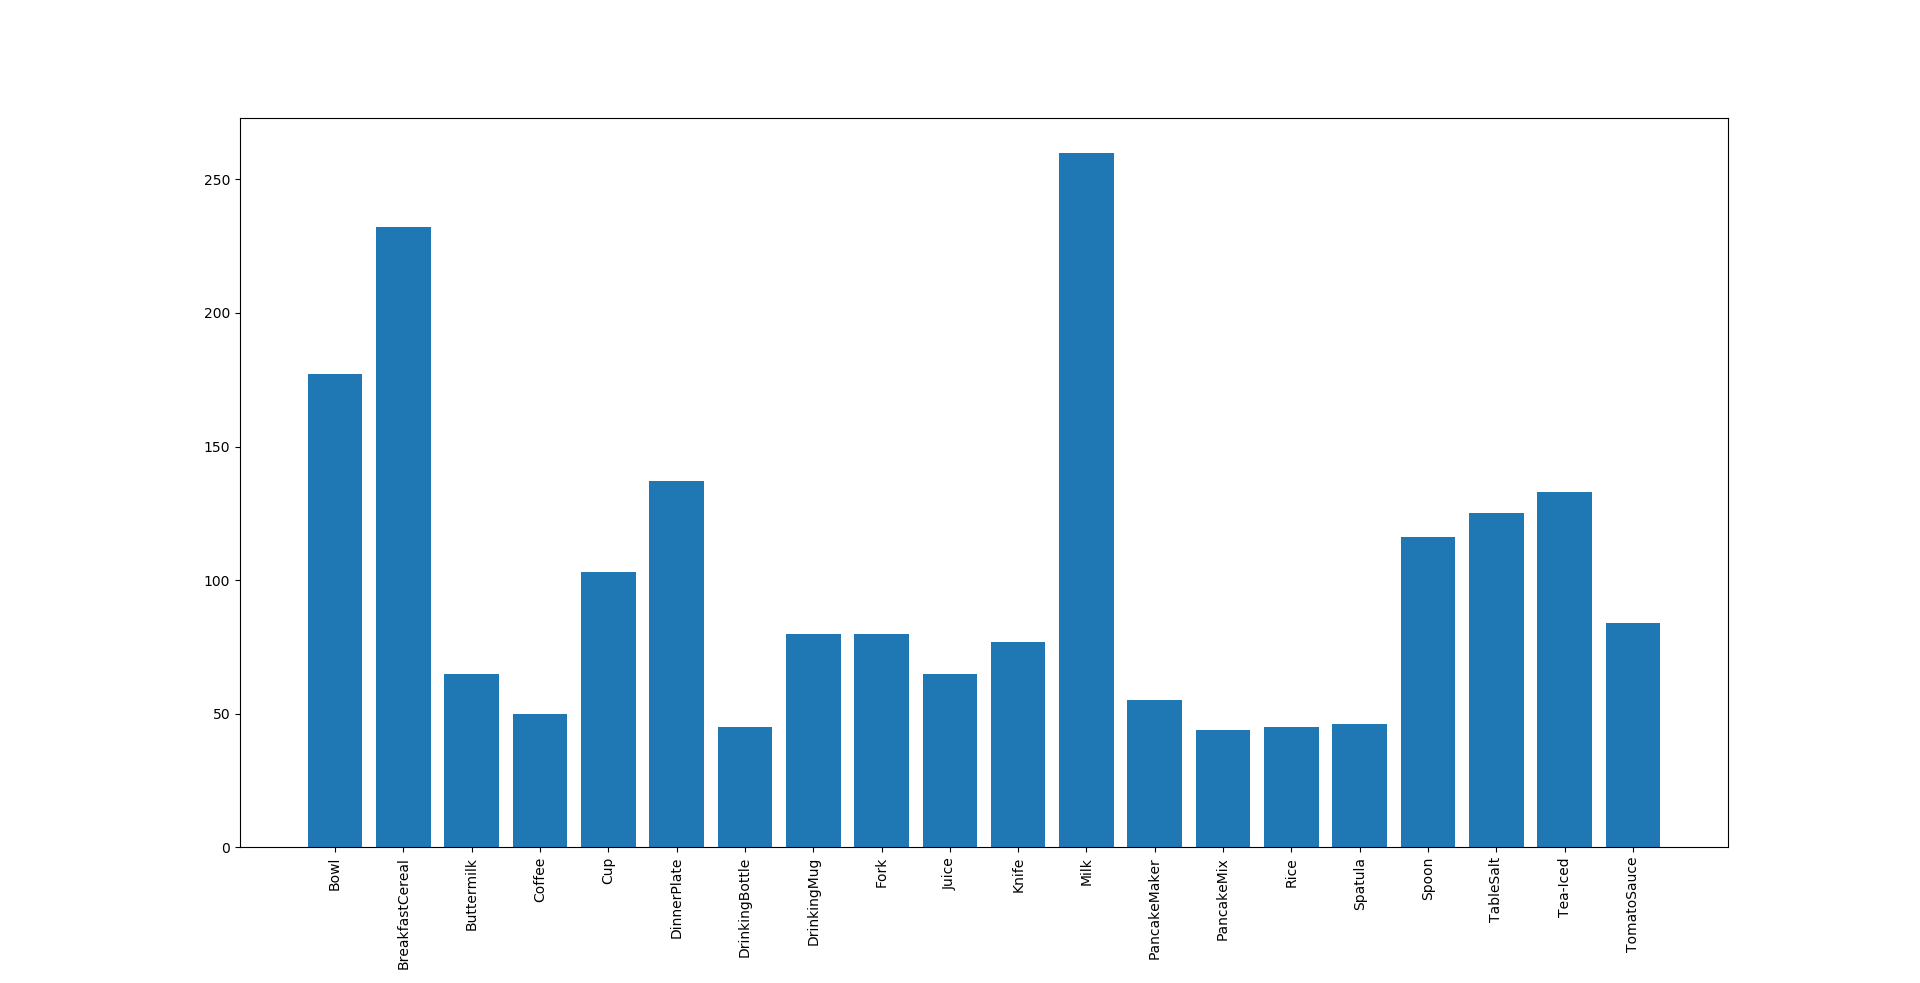
\includegraphics[scale=.4]{img/chapter6/UnrealGTClass_analysis.png}
	\end{subfigure}
	\begin{subfigure}[b]{0.58\textwidth}
	\centering
		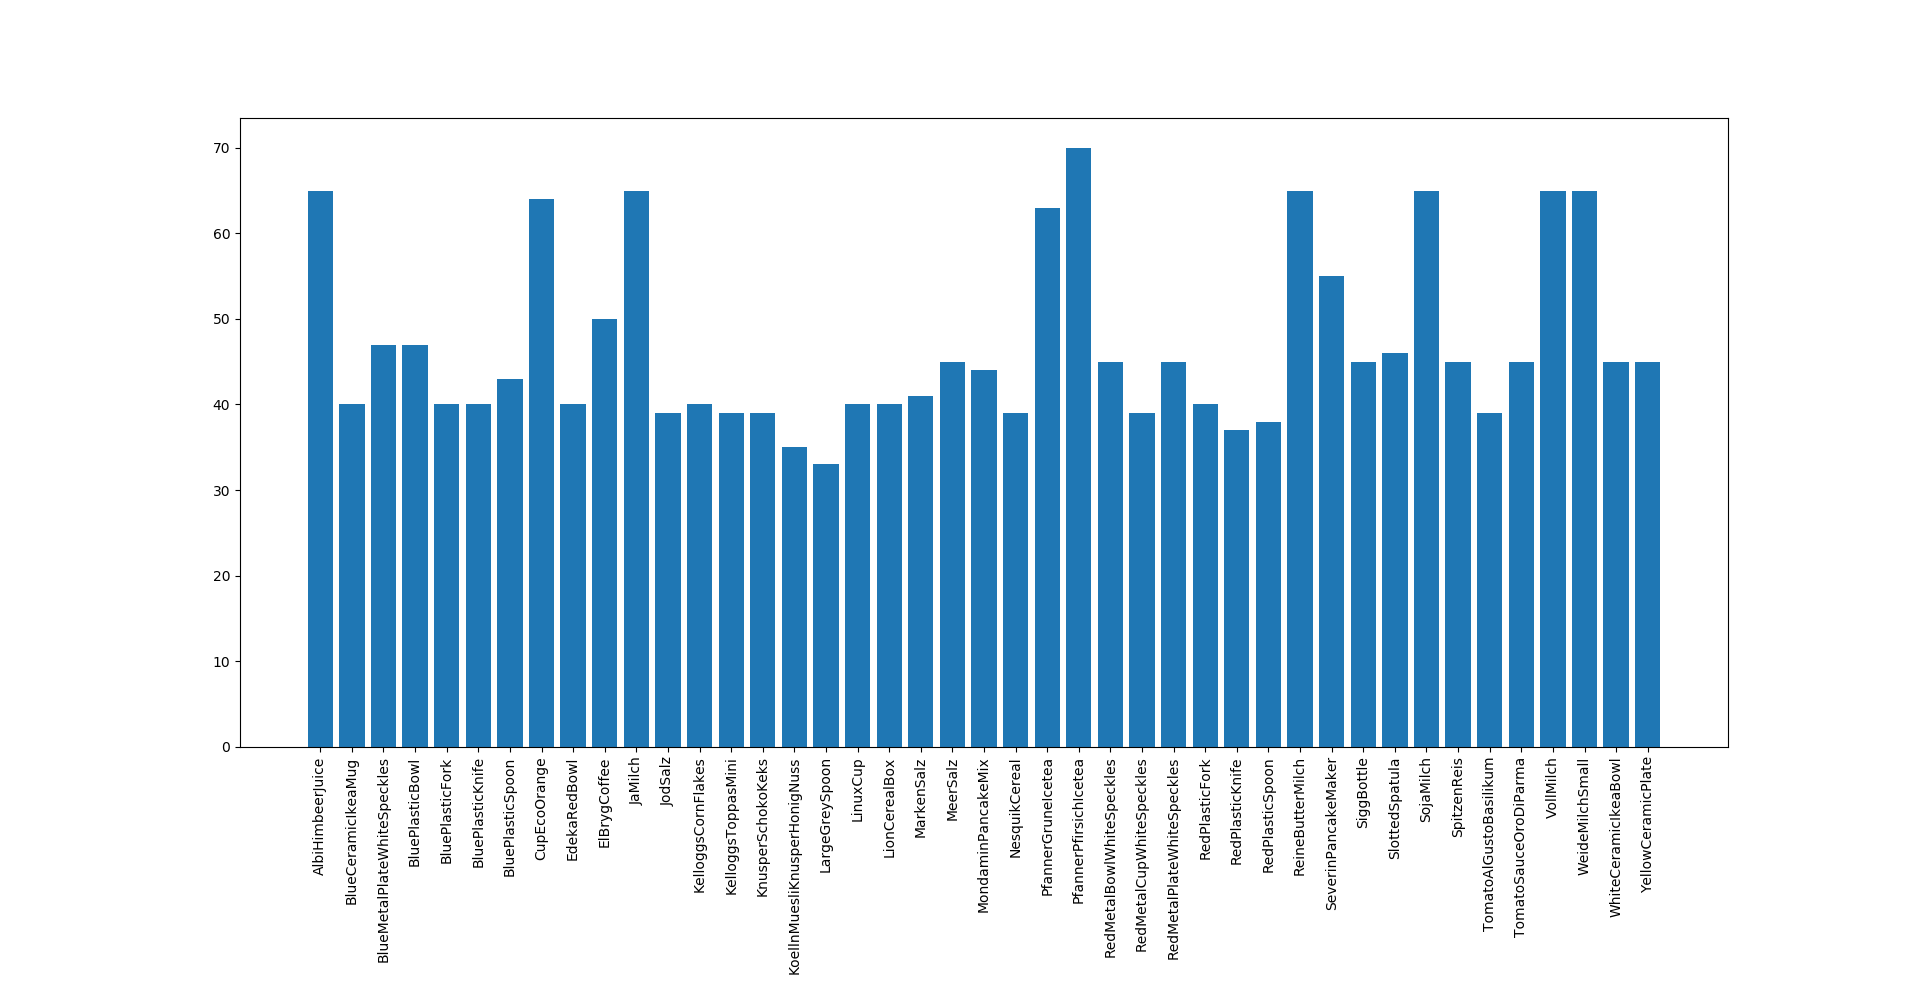
\includegraphics[scale=.4]{img/chapter6/UnrealGTInstance_analysis.png}	
	\end{subfigure}
\caption[Verteilung der Objekte in den Unreal-Bildern]{Verteilung der Objektklassen und Instanzen in den gesamten Unreal-Bildern.}
\label{fig:Unreal-Images_analysis}
\end{figure}

\subsection{Reale Bilder}
Mit dem PR2-Roboter des \gls{iai} wurden Bilder in der realen Küchenumgebung aufgenommen. Die verwendeten Objekte sind dabei die Vorlagen der Assets, also die ursprünglich eingescannten Objekte. Unglücklicherweise stand zu dem Zeitpunkt der Aufnahme der \textit{LinuxCup} und die \textit{YellowPlate} nicht mehr zur Verfügung. Für die \textit{YellowPlate} wurde stattdessen ein weißer Teller als Ersatzobjekt verwendet. Es wurden wieder 114 Szenen mit der gleichen Szenarien-Verteilung und den gleichen Bedingungen erstellt. Auf Grund des erhöhten Aufwandes bei der Aufnahme der Szenen wurden von jeder Szene nur drei Bilder aufgenommen, womit insgesamt \textbf{342 reale Bilder} zur Verfügung stehen. Im Gegensatz zu den Unreal-Bildern sind die Blickwinkel nicht für jede Szene exakt die Gleichen, da der Roboter bei der Aufnahme manuell bewegt werden muss (eine Szene ist in Abbildung \ref{fig:exampleSceneReal} zu sehen). \par

\begin{figure}
\centering
	\begin{subfigure}[b]{0.3\textwidth}
		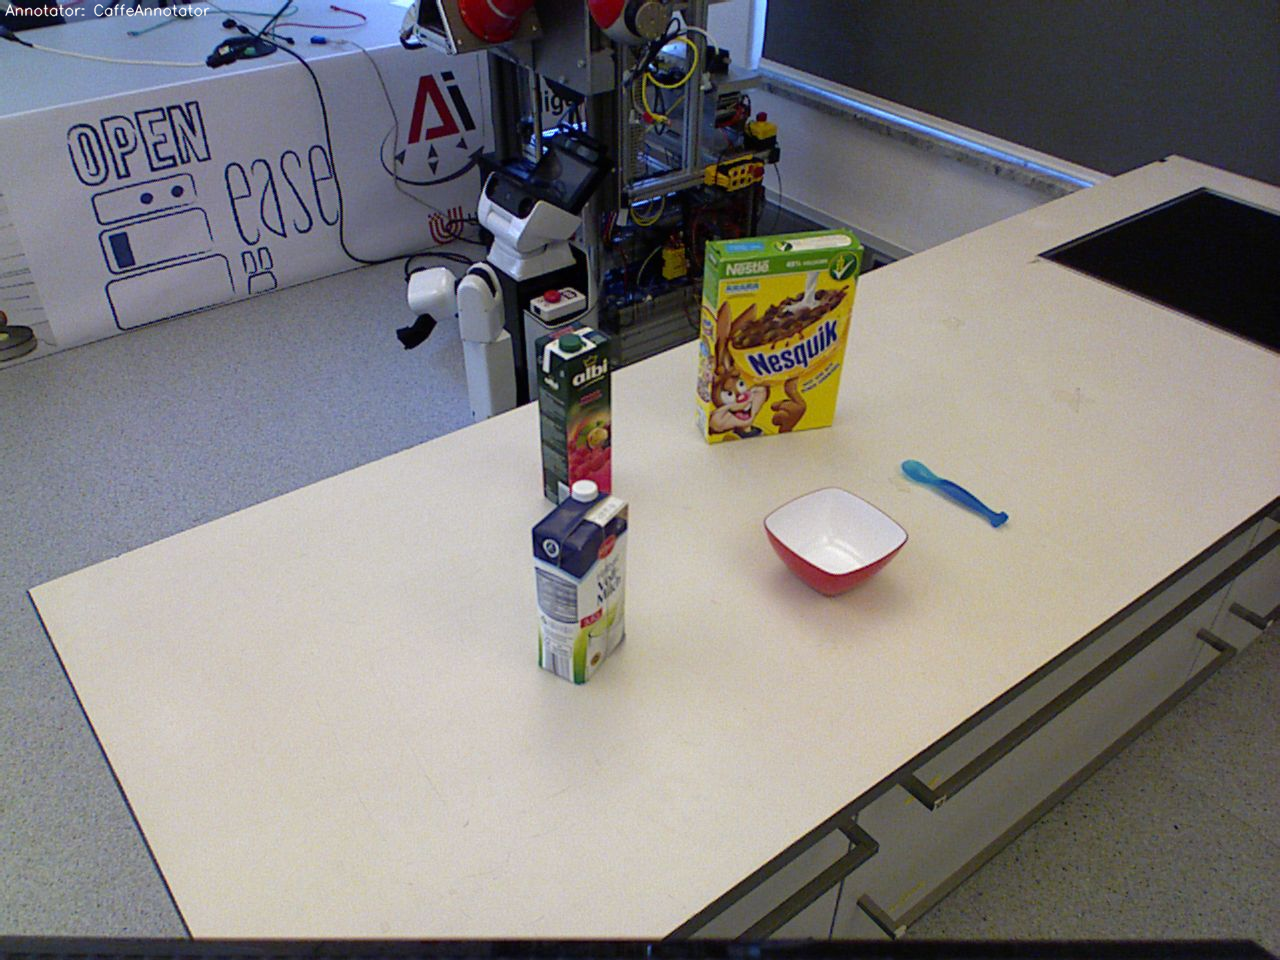
\includegraphics[scale=.1]{img/chapter6/real1}
	\end{subfigure}
	\quad
	\begin{subfigure}[b]{0.3\textwidth}
		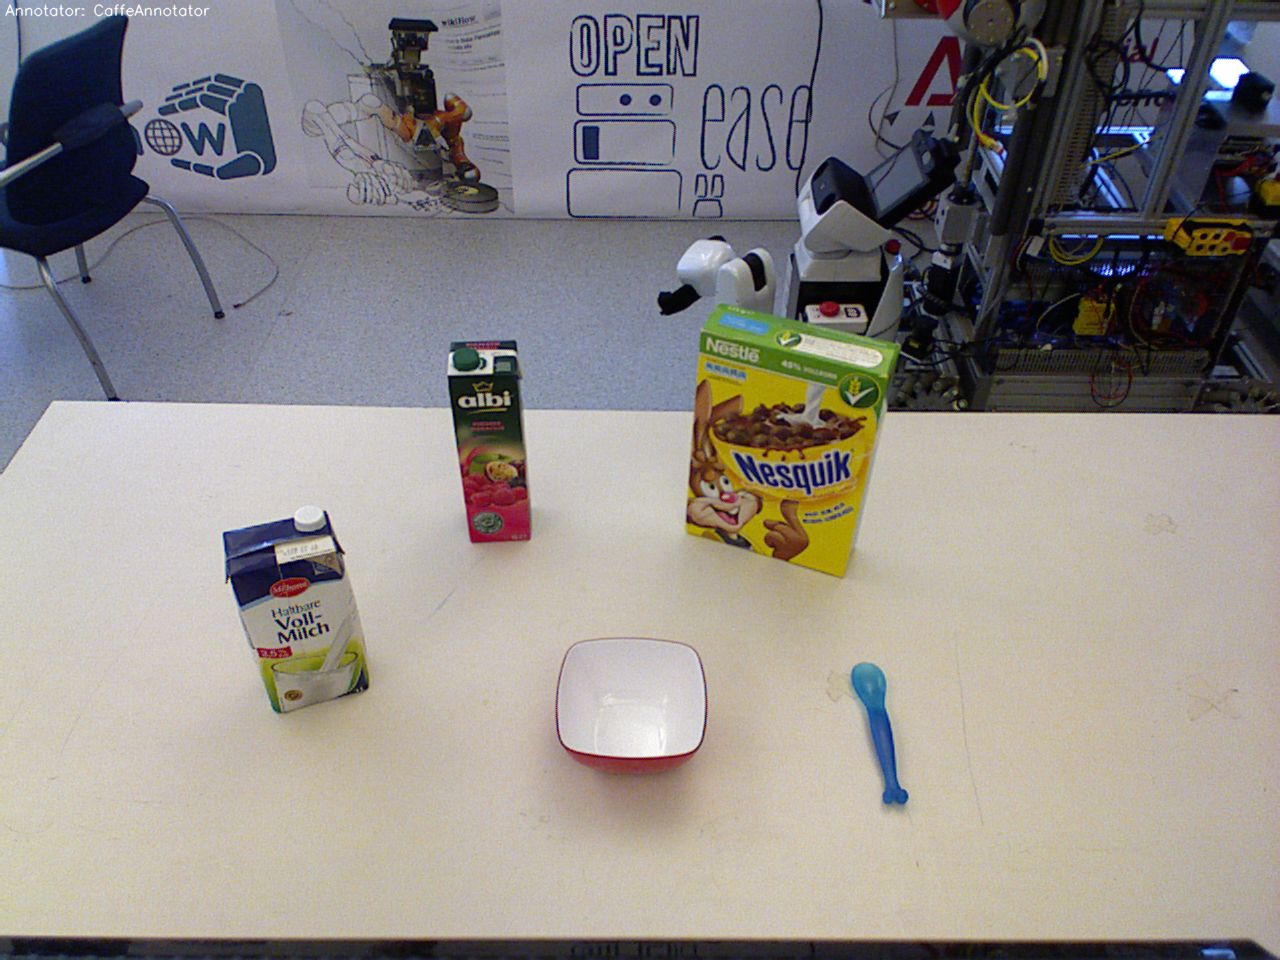
\includegraphics[scale=.1]{img/chapter6/real2}	
	\end{subfigure}
	\quad
	\begin{subfigure}[b]{0.3\textwidth}
		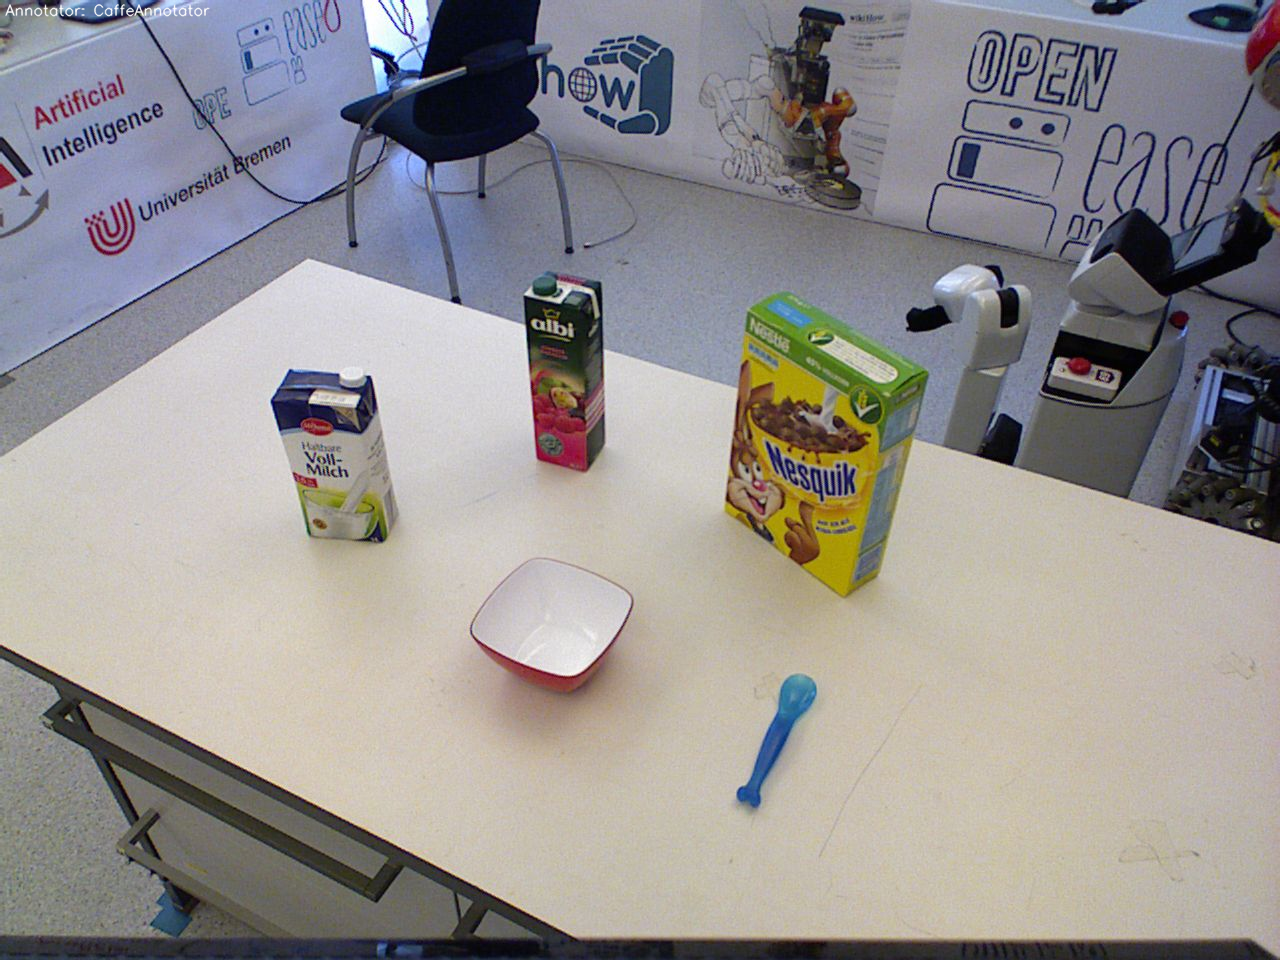
\includegraphics[scale=.1]{img/chapter6/real3}	
	\end{subfigure}
\caption[Reale Bilder einer Szene]{Ein Bildersatz der realen Szenen.}
\label{fig:exampleSceneReal}
\end{figure}

\begin{figure}
\centering
	\begin{subfigure}[b]{0.4\textwidth}
	\centering
		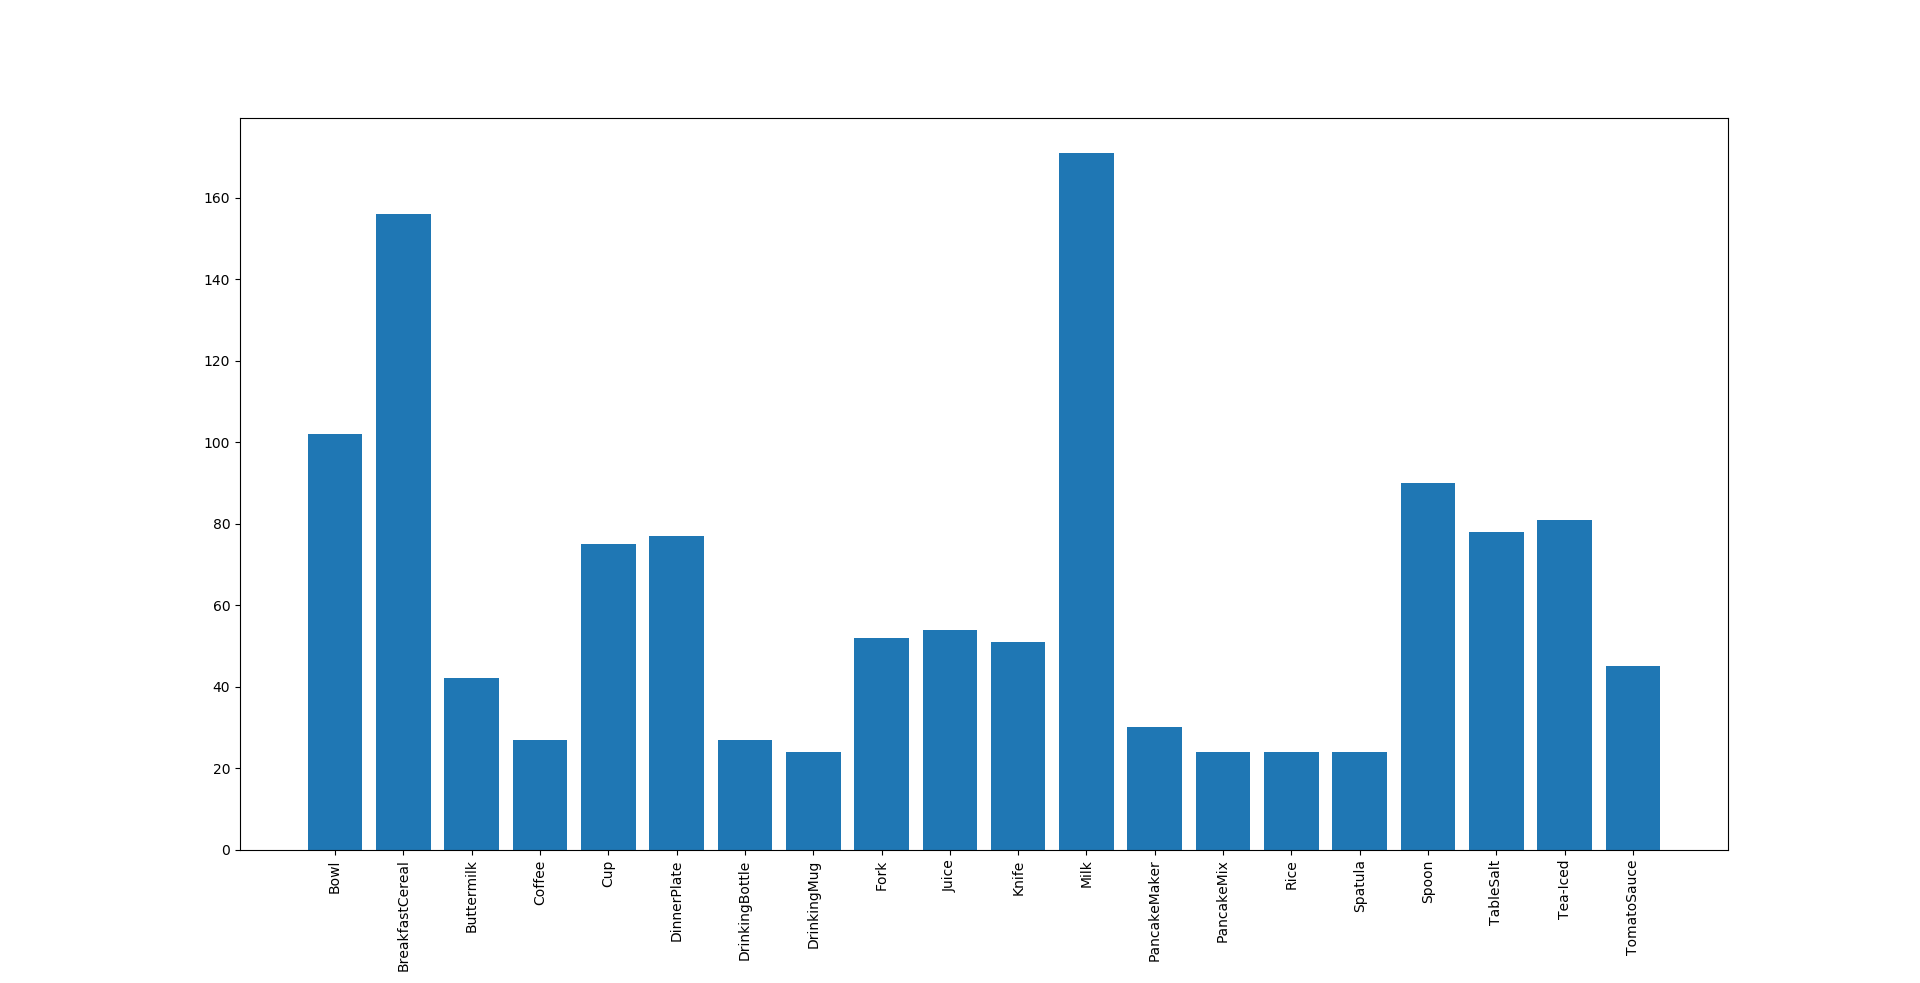
\includegraphics[scale=.4]{img/chapter6/RealGTClass_analysis.png}
	\end{subfigure}
	\begin{subfigure}[b]{0.58\textwidth}
	\centering
		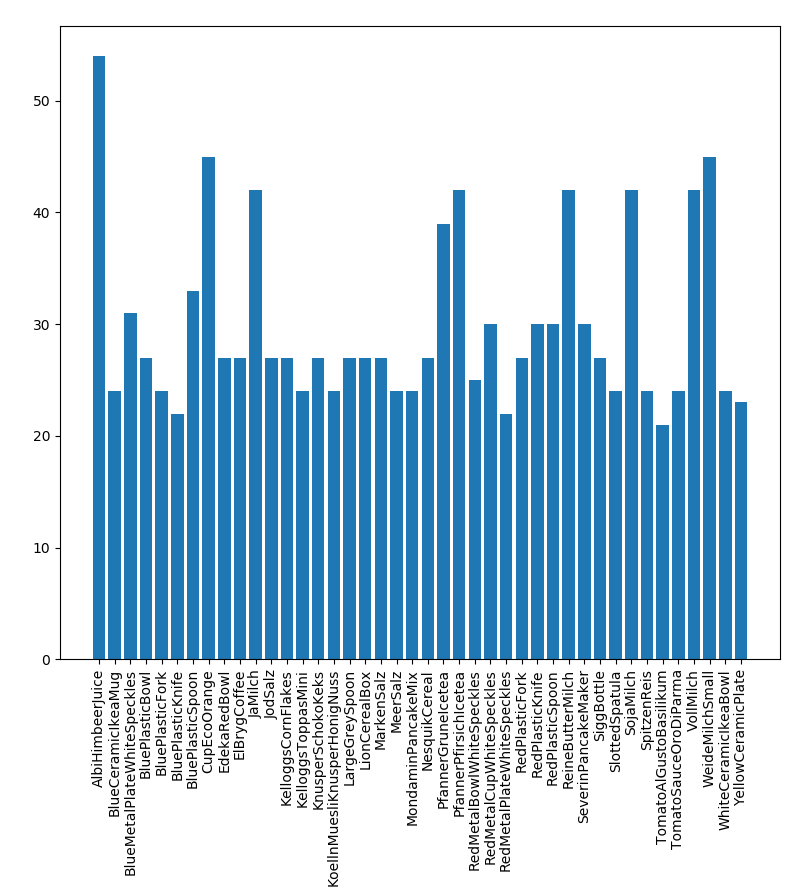
\includegraphics[scale=.4]{img/chapter6/RealGTInstance_analysis.png}	
	\end{subfigure}
\caption[Verteilung der Objekte in den Unreal-Bildern]{Verteilung der Objektklassen und Instanzen in den gesamten Unreal-Bildern.}
\label{fig:Real-Images_analysis}
\end{figure}

Die Verteilung der Objektklassen und Instanzen in den realen Bildern, zu sehen in Abbildung \ref{fig:Real-Images_analysis}, zeigt die gleichen Eigenschaften, wie die Verteilung der Unreal-Bilder. Es wird auch hier von einem ungleich verteilten Datensatz ausgegangen. 

\section{Klassifizierung mit Klassifikatoren}
\label{sec:classificationExperiment}
Die zuvor erstellten Unreal-Bilder wurden in ersten Experimenten über \gls{feature} klassifiziert. Dazu wurde ein Annotator aus dem \robosherlock-Paket \textit{rs\_addons} als \gls{klassifikator} mit echten Bildern der verwendeten Objekte trainiert. Mehr zu dem Paket und den \glspl{klassifikator} ist in Kapitel \ref{sec:classifiers} auf Seite \pageref{sec:classifiers} zu finden. \par

Als \glspl{klassifikator} wurden der \texttt{RFAnnotator} und der \texttt{SVMAnnotator} verwendet, die jeweils auf einer \gls{rf} oder \gls{svm} Implementierung basieren. Die Objekte sollten in zwei Versuchsreihen entweder den Objektklassen oder den Instanznamen zugeordnet werden. Vor dem Training der \glspl{klassifikator} wurden die Bilder der echten Objekte den Klassen/Instanzen zugeordnet. Da es sich um Annotatoren für \robosherlock handelt, wurde eine \gls{ae} mit einigen \textit{hyotheses generators}, dem \texttt{CaffeAnnotator} zum Extrahieren der Merkmale (siehe Kap. \ref{sec:caffeAnno}, S.\pageref{sec:caffeAnno}), dem\linebreak \texttt{UnrealGTAnnotator} zum herausziehen der \gls{gt} aus den Unreal-Bildern und dem jeweiligen \gls{klassifikator} erstellt. Um die Ergebnisse später verarbeiten zu können wurden sie mit dem \texttt{MLNInferencer} (siehe Kap. \ref{sec:mlnInferencer}, S. \pageref{sec:mlnInferencer}) als logische Prädikate ausgegeben. Die so erhaltene Klassifizierung wird für jedes Objekt mit der \gls{gt} verglichen, um so die Klassifikationsrate des \gls{klassifikator}s zu ermitteln.

\subsection{Objektklassen}
Die Ergebnisse des \texttt{RFAnnotators} sind in Abbildung \ref{fig:RFClassifierGTClass_confMatrix} und Tabelle \ref{tab:RFClassifierGTClass_metrics} abgebildet. Während nahezu alle Objekte eine \gls{accuracy} über 90\% aufweisen, zeigen \gls{precision}, \gls{recall} und \gls{f1score}, dass der \texttt{RFAnnotator} große Schwierigkeiten hat, visuell ähnliche Objekte auseinander zu halten. Besonders häufig werden Objekte fälschlicherweise als \textit{Milk} und \textit{TableSalt} eingeordnet. Dies ist auf die box-artige Form und die Farbähnlichkeit vieler Objekte der beiden Klassen zurückzuführen, welche insgesamt auch in größerer Zahl in den Daten vorkommen als andere Objektklassen. Des weiteren hat der \gls{klassifikator} Schwierigkeiten, das Geschirr auseinander zu halten, was auf die Größe dessen zurückzuführen ist. Besonders schlecht schneidet der \textit{Spatula} ab, der nicht einmal korrekt erkannt wurde. Mit einem \gls{f1score} über 80\% schneiden die Objektklassen \textit{Buttermilk}, \textit{Coffee}, \textit{Cup} und \textit{PancakeMix} am besten ab. Diese Klassen unterscheiden sich in Form (\textit{Buttermilk}, \textit{PancakeMix}) und Farbe (\textit{Coffee}, \textit{Cup}) stark von den anderen Objekten.  \par

\begin{figure}
\centering
	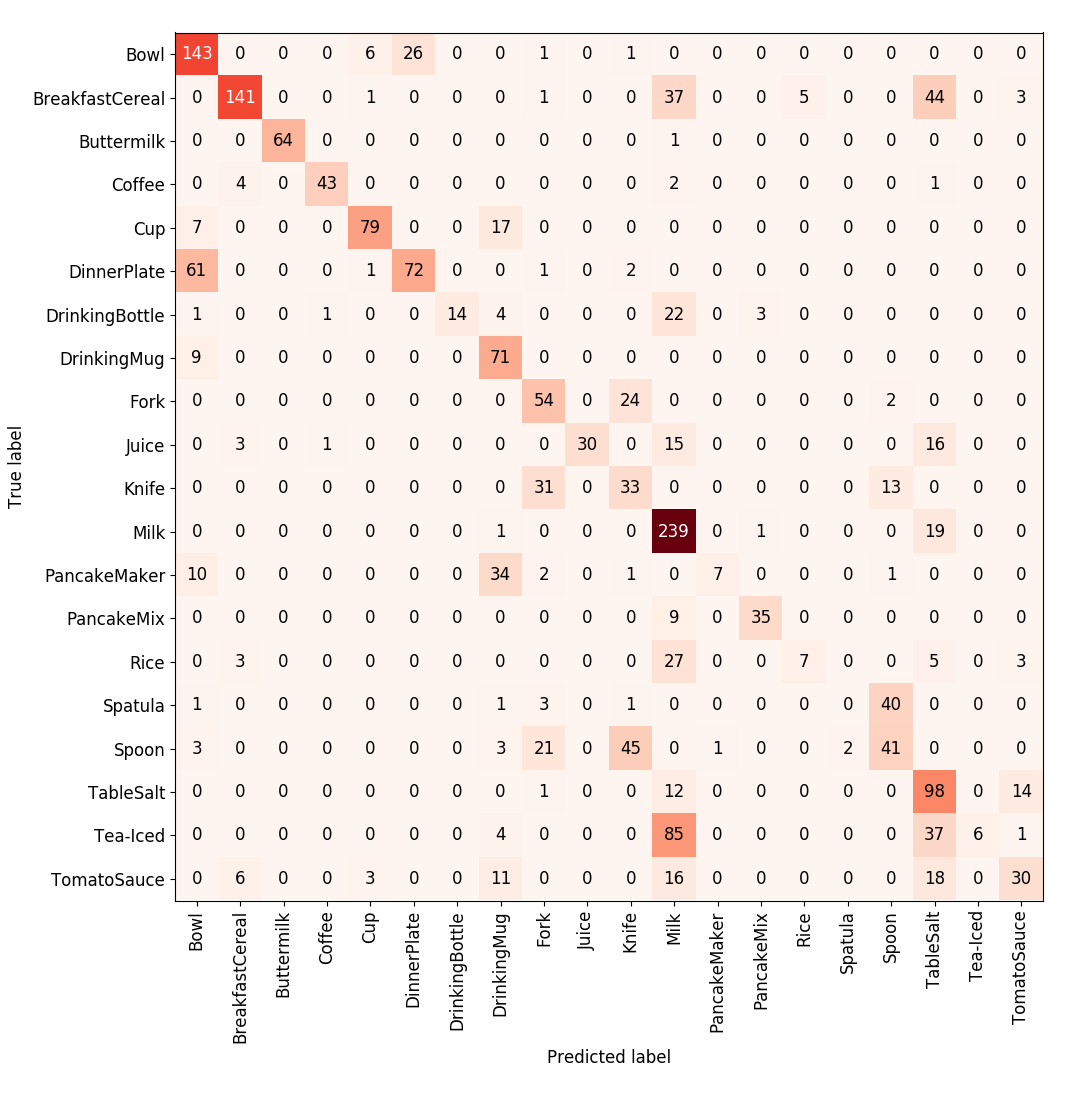
\includegraphics[scale=.315]{img/chapter6/RFClassifierGTClass.png}
\caption[Konfusionsmatrix der Klassifizierung der Objektklassen durch den RFAnnotator]{Die Konfusionsmatrix für die Objektklassen Klassifikation der Unreal-Bilder durch den mit echten Bildern trainierten \texttt{RFAnnotator}.}
\label{fig:RFClassifierGTClass_confMatrix}
\end{figure}

\begin{table}
\centering
\small
\rowcolors{1}{}{lightgray}
\begin{tabularx}{\textwidth}{Xllll}
\textbf{Objekt}	& \textbf{\gls{accuracy}} & \textbf{\gls{precision}}	& \textbf{\gls{recall}}	& \textbf{\gls{f1score}} \\ \hline
Bowl & 0.91 & 0.61 & 0.81 & 0.69 \\  
BreakfastCereal & 0.92 & 0.9 & 0.61 & 0.72 \\  
Buttermilk & 1.0 & 1.0 & 0.98 & 0.99 \\  
Coffee & 0.99 & 0.96 & 0.86 & 0.91 \\  
Cup & 0.97 & 0.88 & 0.77 & 0.82 \\  
DinnerPlate & 0.93 & 0.73 & 0.53 & 0.61 \\  
DrinkingBottle & 0.97 & 1.0 & 0.31 & 0.47 \\  
DrinkingMug & 0.93 & 0.49 & 0.89 & 0.63 \\  
Fork & 0.93 & 0.47 & 0.68 & 0.55 \\  
Juice & 0.97 & 1.0 & 0.46 & 0.63 \\  
Knife & 0.91 & 0.31 & 0.43 & 0.36 \\  
Milk & 0.83 & 0.51 & 0.92 & 0.66 \\  
PancakeMaker & 0.96 & 0.88 & 0.13 & 0.22 \\  
PancakeMix & 0.99 & 0.9 & 0.8 & 0.84 \\  
Rice & 0.97 & 0.58 & 0.16 & 0.25 \\  
Spatula & 0.96 & 0.0 & 0.0 & 0.0 \\  
Spoon & 0.9 & 0.42 & 0.35 & 0.38 \\  
TableSalt & 0.88 & 0.41 & 0.78 & 0.54 \\  
Tea-Iced & 0.9 & 1.0 & 0.05 & 0.09 \\  
TomatoSauce & 0.94 & 0.59 & 0.36 & 0.44 \\  \hline
\textbf{Gesamt}		&	\textbf{0.6}   &	\textbf{0.67}  & \textbf{0.6}     &  \textbf{0.57}     \\
\end{tabularx}
\caption[Objektklassen-spezifische Kenngrößen des RFAnnotators]{Kenngrößen für die einzelnen Objekte aus der Objektklassen Klassifizierung der Unreal-Bilder mit dem \texttt{RFAnnotator}.}
\label{tab:RFClassifierGTClass_metrics}
\end{table}

Die Ergebnisse des \texttt{SVMAnnotators} sind in Abbildung  \ref{fig:SVMClassifierGTClass_confMatrix} zu sehen. Insgesamt sind die Ergebnisse gegenüber dem \texttt{RFAnnotator} etwas besser, da der \texttt{SVMAnnotator} mit 62\% eine etwas höhere \gls{accuracy} aufweist. Jedoch werden vom \texttt{SVMAnnotator} neben dem \textit{Spatula} auch der \textit{PancakeMaker} gar nicht richtig eingeordnet und auch die \textit{DrinkingBottle} schneidet sehr schlecht ab. Der \texttt{SVMAnnotator} ist insgesamt bei einigen Klassen etwas zuverlässiger, hat jedoch auch einige größere Fehlerquellen, was insgesamt zu dem gleichen \gls{f1score} des \texttt{RFAnnotators} von 57\% führt.  

\begin{figure}
\centering
	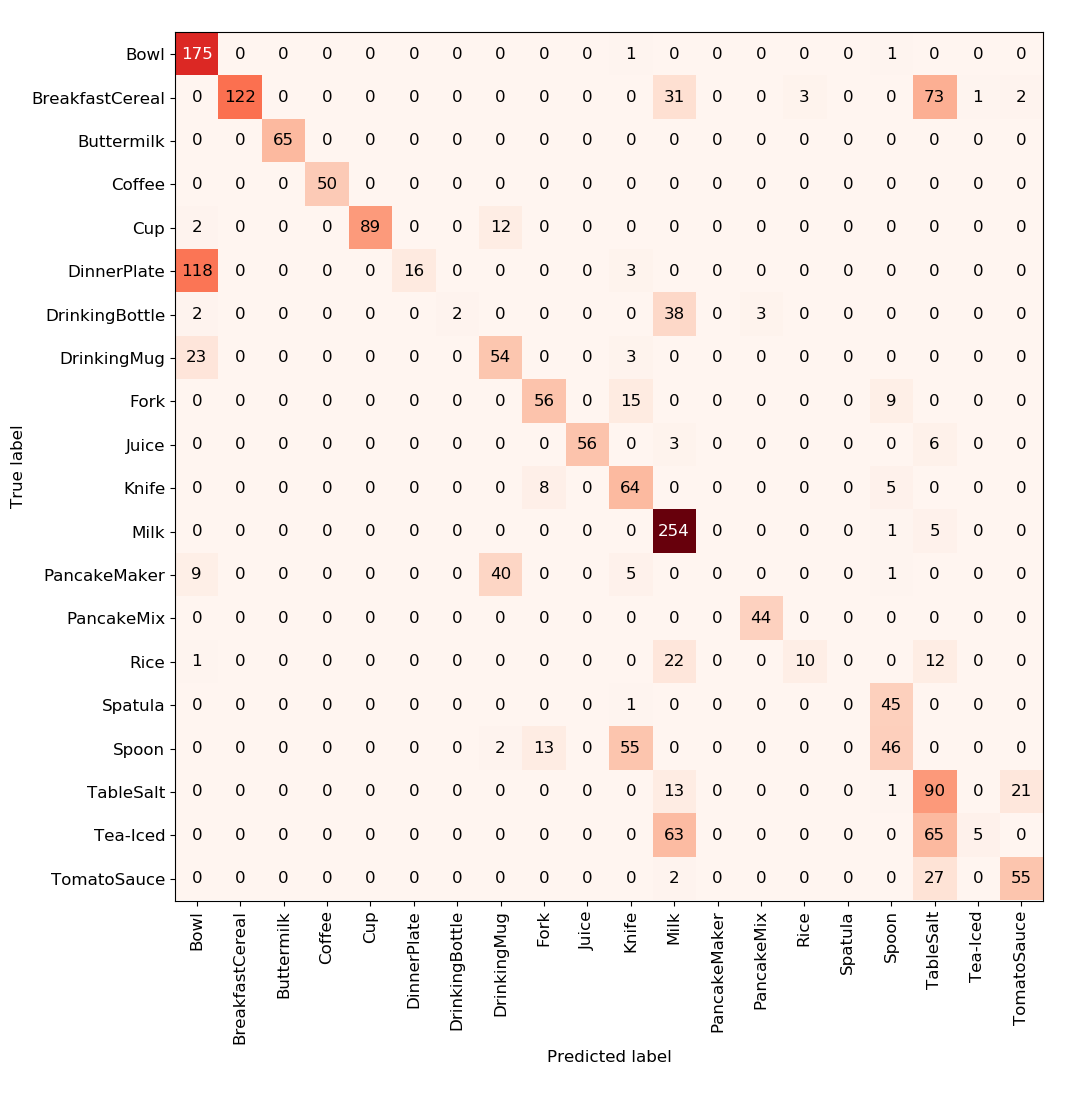
\includegraphics[scale=.315]{img/chapter6/SVMClassifierGTClass.png}
\caption[Konfusionsmatrix der Klassifizierung der Objektklassen durch den SVMAnnotator]{Die Konfusionsmatrix für die Objektklassen Klassifikation der Unreal-Bilder durch den mit echten Bildern trainierten \texttt{SVMAnnotator}.}
\label{fig:SVMClassifierGTClass_confMatrix}
\end{figure}

\begin{table}
\centering
\small
\rowcolors{1}{}{lightgray}
\begin{tabularx}{\textwidth}{Xllll}
\textbf{Objekt}	& \textbf{\gls{accuracy}} & \textbf{\gls{precision}}	& \textbf{\gls{recall}}	& \textbf{\gls{f1score}} \\ \hline
Bowl & 0.89 & 0.53 & 0.99 & 0.69 \\  
BreakfastCereal & 0.92 & 1.0 & 0.53 & 0.69 \\  
Buttermilk & 1.0 & 1.0 & 1.0 & 1.0 \\  
Coffee & 1.0 & 1.0 & 1.0 & 1.0 \\  
Cup & 0.99 & 1.0 & 0.86 & 0.93 \\  
DinnerPlate & 0.91 & 1.0 & 0.12 & 0.21 \\  
DrinkingBottle & 0.97 & 1.0 & 0.04 & 0.09 \\  
DrinkingMug & 0.94 & 0.5 & 0.68 & 0.57 \\  
Fork & 0.97 & 0.73 & 0.7 & 0.71 \\  
Juice & 0.99 & 1.0 & 0.86 & 0.93 \\  
Knife & 0.93 & 0.44 & 0.83 & 0.57 \\  
Milk & 0.88 & 0.6 & 0.98 & 0.74 \\  
PancakeMaker & 0.96 & 0.0 & 0.0 & 0.0 \\  
PancakeMix & 1.0 & 0.94 & 1.0 & 0.97 \\  
Rice & 0.97 & 0.77 & 0.22 & 0.34 \\  
Spatula & 0.96 & 0.0 & 0.0 & 0.0 \\  
Spoon & 0.9 & 0.42 & 0.4 & 0.41 \\  
TableSalt & 0.85 & 0.32 & 0.72 & 0.45 \\  
Tea-Iced & 0.91 & 0.83 & 0.04 & 0.07 \\  
TomatoSauce & 0.96 & 0.71 & 0.65 & 0.68 \\    \hline
\textbf{Gesamt}		&	\textbf{0.62}   &	\textbf{0.7}  & \textbf{0.62}     &  \textbf{0.57}     \\
\end{tabularx}
\caption[Objektklassen-spezifische Kenngrößen des SVMAnnotators]{Kenngrößen für die einzelnen Objekte aus der Objektklassen Klassifizierung der Unreal-Bilder mit dem \texttt{SVMAnnotator}.}
\label{tab:SVMClassifierGTClass_metrics}
\end{table}

\subsection{Instanznamen}

\begin{figure}
\centering
	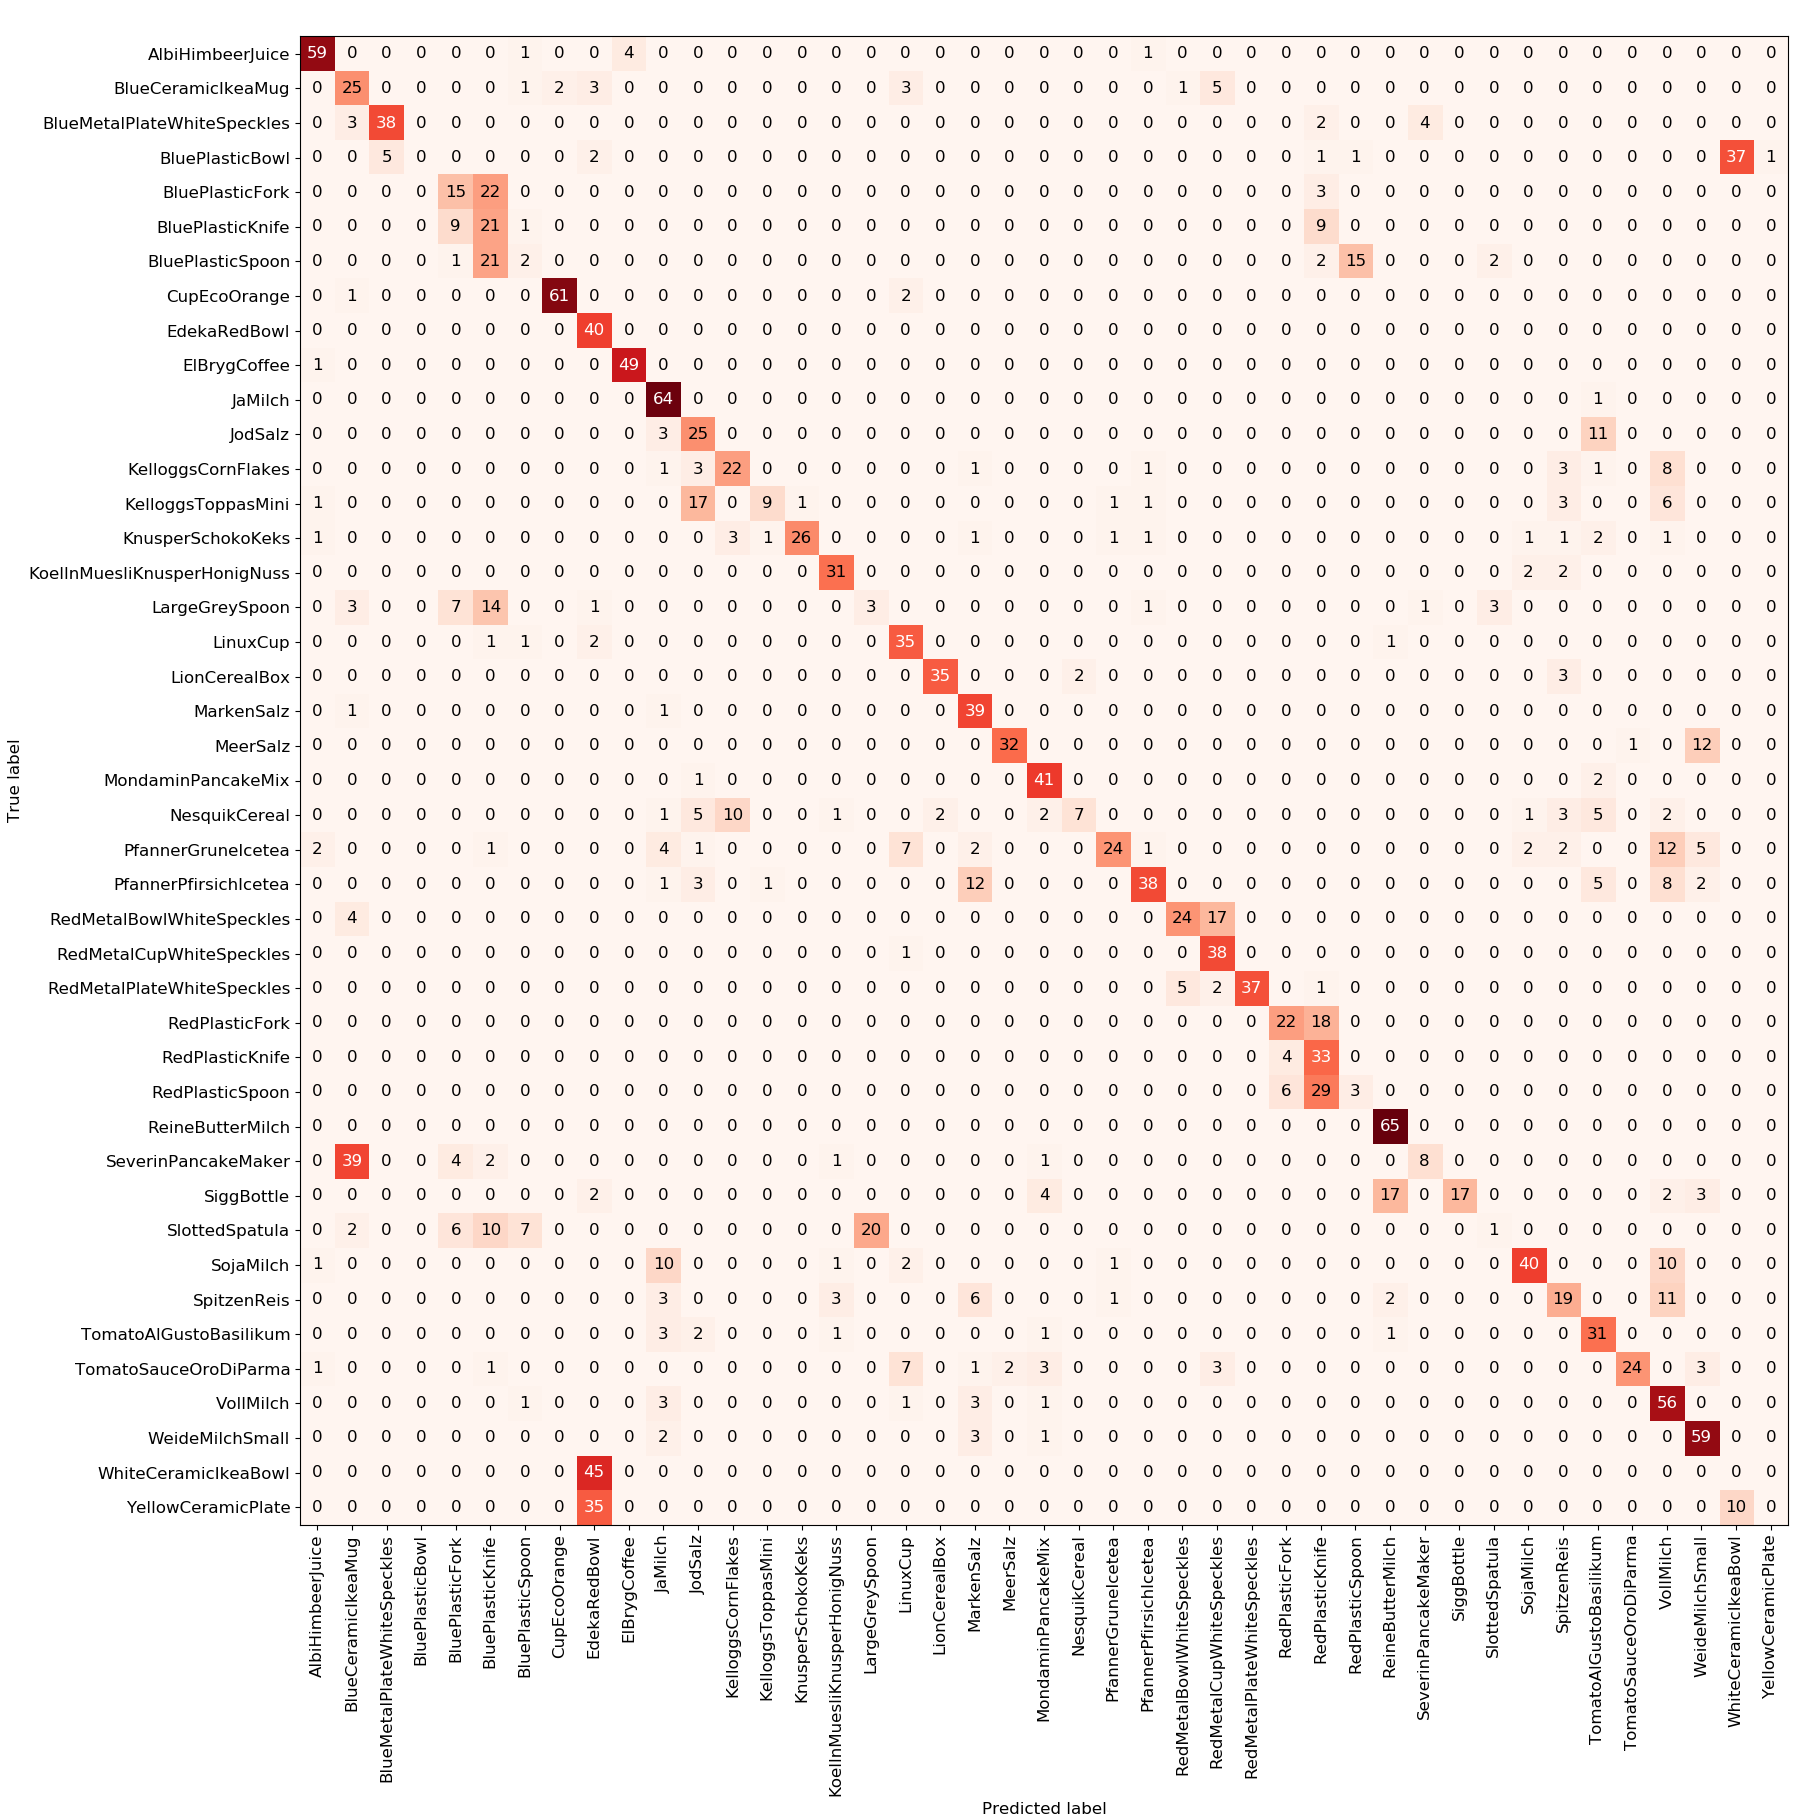
\includegraphics[scale=.292]{img/chapter6/RFClassifierGTInstance.png}
\caption[Konfusionsmatrix der Klassifizierung der Objektinstanzen durch den RFAnnotator]{Die Konfusionsmatrix für die Objektinstanzen Klassifikation der Unreal-Bilder durch den mit echten Bildern trainierten \texttt{RFAnnotator}.}
\label{fig:RFClassifierGTInstance_confMatrix}
\end{figure}

Die Ergebnisse der Instanzenklassifikation des \texttt{RFAnnotators} sind in Abbildung \ref{fig:RFClassifierGTInstance_confMatrix} und Tabelle \ref{tab:RFClassifierGTInstance_metrics} zu finden. Grundsätzlich lässt sich sagen, dass die Klassifikationsrate nahezu identisch ist. Die Fehler bei den Klassen wurden auf die Instanzen übertragen, wodurch nun zu erkennen ist, welche Instanzen die Fehler verursachen. Beispielsweise wird der \textit{SlottedSpatula} in der Hälfte der der Fälle für den \textit{LargeGreySpoon} gehalten. Da beide sich ähnlich sehen, ist dies keine Überraschung, zeigt jedoch auch, dass \texttt{RFAnnotator} mit dieser Ähnlichkeit nicht umgehen kann. In den anderen Fällen ist er einem der blauen Geschirrteile zugeordnet, nicht den Roten. \newline
Interessanterweise werden sowohl die \textit{BluePlasticBowl} als auch die \textit{WhiteCeramicIkeaBowl} nicht einmal richtig erkannt. Erstere wird häufig für Letztere gehalten. Die IkeaBowl stattdessen für die \textit{EdekaRedBowl}. Dies fiel bei der Klassifikation mit Objektklassen noch nicht auf, da alle unter \textit{Bowl} zusammengefasst sind und so trotzdem richtig eingeordnet wurden.   

\begin{table}
\centering
\small
\rowcolors{1}{}{lightgray}
\begin{tabularx}{\textwidth}{Xllll}
\textbf{Objekt}	& \textbf{\gls{accuracy}} & \textbf{\gls{precision}}	& \textbf{\gls{recall}}	& \textbf{\gls{f1score}} \\ \hline
AlbiHimbeerJuice & 0.99 & 0.89 & 0.91 & 0.9 \\  
BlueCeramicIkeaMug & 0.95 & 0.32 & 0.63 & 0.42 \\  
BlueMetalPlateWhiteSpeckles & 0.99 & 0.88 & 0.81 & 0.84 \\  
BluePlasticBowl & 0.96 & 0.0 & 0.0 & 0.0 \\  
BluePlasticFork & 0.96 & 0.36 & 0.38 & 0.37 \\  
BluePlasticKnife & 0.93 & 0.23 & 0.53 & 0.32 \\  
BluePlasticSpoon & 0.96 & 0.14 & 0.05 & 0.07 \\  
CupEcoOrange & 1.0 & 0.97 & 0.95 & 0.96 \\  
EdekaRedBowl & 0.93 & 0.31 & 1.0 & 0.47 \\  
ElBrygCoffee & 1.0 & 0.92 & 0.98 & 0.95 \\  
JaMilch & 0.97 & 0.67 & 0.98 & 0.8 \\  
JodSalz & 0.96 & 0.44 & 0.64 & 0.52 \\  
KelloggsCornFlakes & 0.98 & 0.63 & 0.55 & 0.59 \\  
KelloggsToppasMini & 0.97 & 0.82 & 0.23 & 0.36 \\  
KnusperSchokoKeks & 0.99 & 0.96 & 0.67 & 0.79 \\  
KoellnMuesliKnusperHonigNuss & 0.99 & 0.82 & 0.89 & 0.85 \\  
LargeGreySpoon & 0.96 & 0.13 & 0.09 & 0.11 \\  
LinuxCup & 0.98 & 0.6 & 0.88 & 0.71 \\  
LionCerealBox & 0.99 & 0.95 & 0.88 & 0.91 \\  
MarkenSalz & 0.98 & 0.57 & 0.95 & 0.72 \\  
MeerSalz & 0.99 & 0.94 & 0.71 & 0.81 \\  
MondaminPancakeMix & 0.99 & 0.76 & 0.93 & 0.84 \\  
NesquikCereal & 0.97 & 0.78 & 0.18 & 0.29 \\  
PfannerGruneIcetea & 0.97 & 0.86 & 0.38 & 0.53 \\  
PfannerPfirsichIcetea & 0.97 & 0.86 & 0.54 & 0.67 \\  
RedMetalBowlWhiteSpeckles & 0.98 & 0.8 & 0.53 & 0.64 \\  
RedMetalCupWhiteSpeckles & 0.98 & 0.58 & 0.97 & 0.73 \\  
RedMetalPlateWhiteSpeckles & 0.99 & 1.0 & 0.82 & 0.9 \\  
RedPlasticFork & 0.98 & 0.69 & 0.55 & 0.61 \\  
RedPlasticKnife & 0.95 & 0.34 & 0.89 & 0.49 \\  
RedPlasticSpoon & 0.96 & 0.16 & 0.08 & 0.11 \\  
ReineButterMilch & 0.98 & 0.76 & 1.0 & 0.86 \\  
SeverinPancakeMaker & 0.96 & 0.62 & 0.15 & 0.24 \\  
SiggBottle & 0.98 & 1.0 & 0.38 & 0.55 \\  
SlottedSpatula & 0.96 & 0.17 & 0.02 & 0.04 \\  
SojaMilch & 0.98 & 0.87 & 0.62 & 0.72 \\  
SpitzenReis & 0.97 & 0.53 & 0.42 & 0.47 \\  
TomatoAlGustoBasilikum & 0.97 & 0.53 & 0.79 & 0.64 \\  
TomatoSauceOroDiParma & 0.98 & 0.96 & 0.53 & 0.69 \\  
VollMilch & 0.95 & 0.48 & 0.86 & 0.62 \\  
WeideMilchSmall & 0.98 & 0.7 & 0.91 & 0.79 \\  
WhiteCeramicIkeaBowl & 0.93 & 0.0 & 0.0 & 0.0 \\  
YellowCeramicPlate & 0.96 & 0.0 & 0.0 & 0.0 \\   \hline
\textbf{Gesamt}		&	\textbf{0.6}   &	\textbf{0.62}  & \textbf{0.6}     &  \textbf{0.58}     \\
\end{tabularx}
\caption[Objektinstanzen-spezifische Kenngrößen des RFAnnotators]{Kenngrößen für die einzelnen Objekte aus der Objektinstanzen Klassifizierung der Unreal-Bilder mit dem \texttt{RFAnnotator}.}
\label{tab:RFClassifierGTInstance_metrics}
\end{table}

Der \texttt{SVMAnnotator} schneidet bei den Instanzen etwas besser ab als bei den Klassen. Dementsprechend auch besser als der \texttt{RFAnnotator} bei den Instanzen. Auch hier sind die Fehler aus der Klassenklassifikation übertragbar. Die \textit{SiggBottle} wird selten erkannt oder als \textit{ReineButterMilch} oder \textit{MondaminPancakeMix} eingeordnet. Zu Verwirrung kommt es hier wahrscheinlich durch deren runde Form und ähnlich helle Farbe. Auch erwähnt seien die sehr schlechten Werte für die beiden farbigen Löffel bei beiden Annotatoren, während die jeweiligen Messer und Gabeln besser abschneiden. Insgesamt sind die Fehlerquellen jedoch wieder nahezu deckungsgleich mit dem \texttt{RFAnnotator}.

\begin{figure}
\centering
	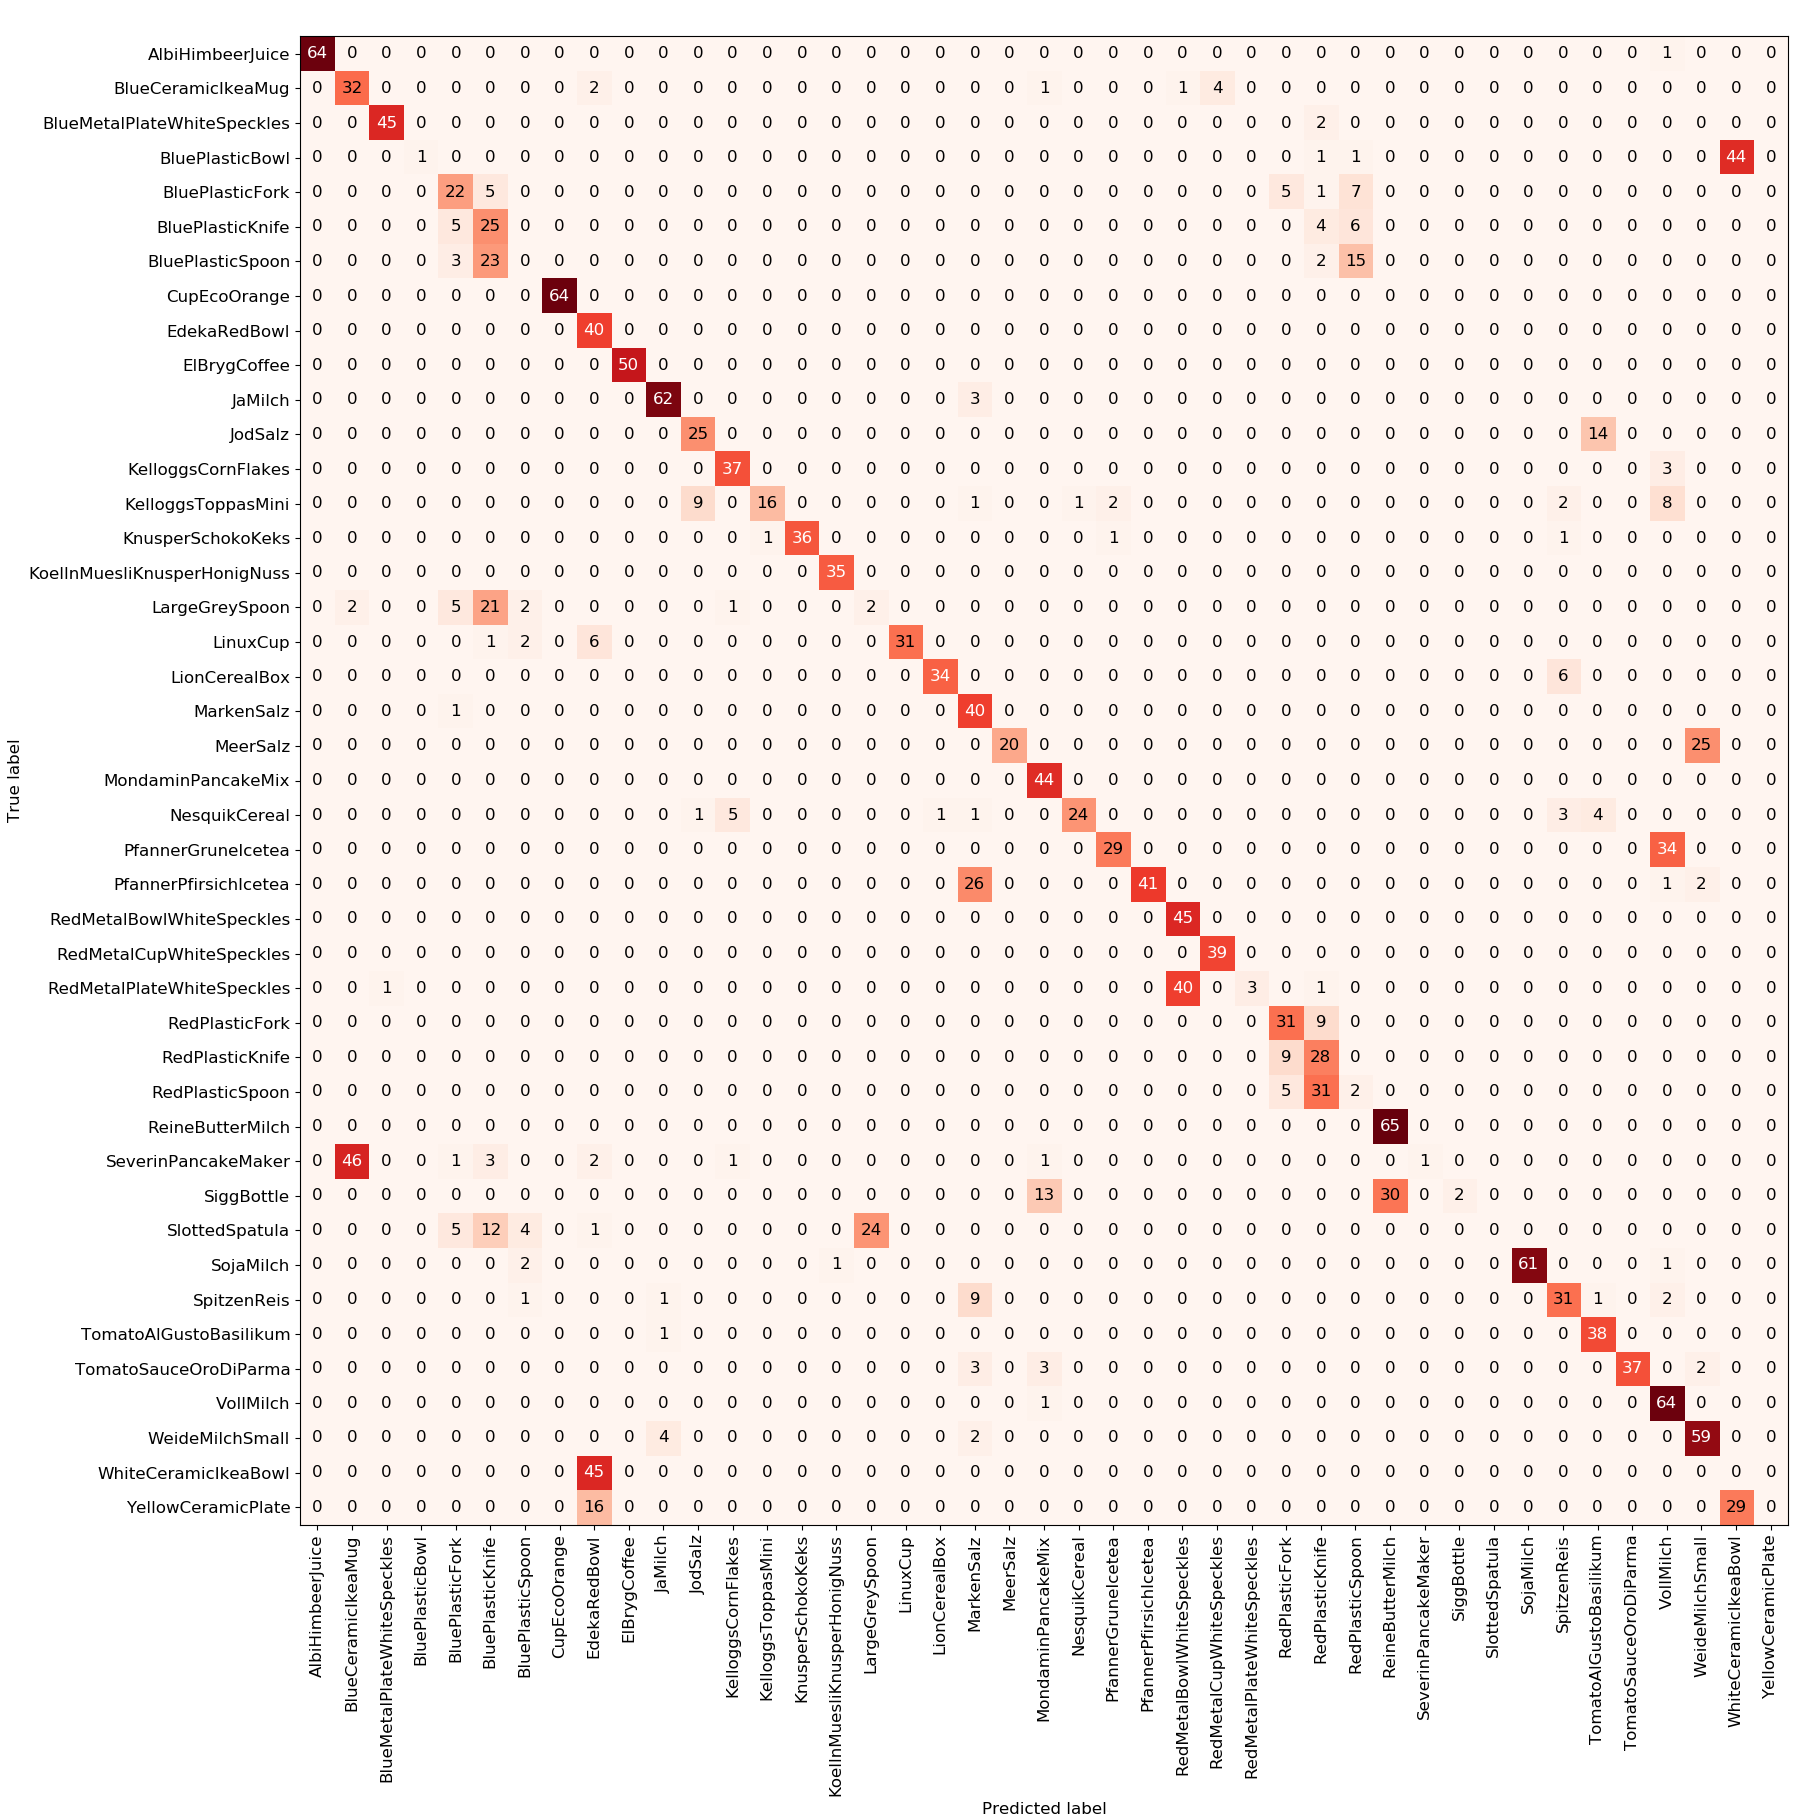
\includegraphics[scale=.292]{img/chapter6/SVMClassifierGTInstance.png}
\caption[Konfusionsmatrix der Klassifizierung der Objektinstanzen durch den SVMAnnotator]{Die Konfusionsmatrix für die Objektinstanzen Klassifikation der Unreal-Bilder durch den mit echten Bildern trainierten \texttt{SVMAnnotator}.}
\label{fig:SVMClassifierGTInstance_confMatrix}
\end{figure}

\begin{table}
\centering
\small
\rowcolors{1}{}{lightgray}
\begin{tabularx}{\textwidth}{Xllll}
\textbf{Objekt}	& \textbf{\gls{accuracy}} & \textbf{\gls{precision}}	& \textbf{\gls{recall}}	& \textbf{\gls{f1score}} \\ \hline
AlbiHimbeerJuice & 1.0 & 1.0 & 0.98 & 0.99 \\  
BlueCeramicIkeaMug & 0.96 & 0.4 & 0.8 & 0.53 \\  
BlueMetalPlateWhiteSpeckles & 1.0 & 0.98 & 0.96 & 0.97 \\  
BluePlasticBowl & 0.97 & 1.0 & 0.02 & 0.04 \\  
BluePlasticFork & 0.97 & 0.52 & 0.55 & 0.54 \\  
BluePlasticKnife & 0.94 & 0.28 & 0.63 & 0.38 \\  
BluePlasticSpoon & 0.96 & 0.0 & 0.0 & 0.0 \\  
CupEcoOrange & 1.0 & 1.0 & 1.0 & 1.0 \\  
EdekaRedBowl & 0.95 & 0.36 & 1.0 & 0.53 \\  
ElBrygCoffee & 1.0 & 1.0 & 1.0 & 1.0 \\  
JaMilch & 0.99 & 0.91 & 0.95 & 0.93 \\  
JodSalz & 0.98 & 0.71 & 0.64 & 0.68 \\  
KelloggsCornFlakes & 0.99 & 0.84 & 0.93 & 0.88 \\  
KelloggsToppasMini & 0.98 & 0.94 & 0.41 & 0.57 \\  
KnusperSchokoKeks & 1.0 & 1.0 & 0.92 & 0.96 \\  
KoellnMuesliKnusperHonigNuss & 1.0 & 0.97 & 1.0 & 0.99 \\  
LargeGreySpoon & 0.96 & 0.08 & 0.06 & 0.07 \\  
LinuxCup & 0.99 & 1.0 & 0.78 & 0.87 \\  
LionCerealBox & 0.99 & 0.97 & 0.85 & 0.91 \\  
MarkenSalz & 0.97 & 0.47 & 0.98 & 0.63 \\  
MeerSalz & 0.98 & 1.0 & 0.44 & 0.62 \\  
MondaminPancakeMix & 0.99 & 0.7 & 1.0 & 0.82 \\  
NesquikCereal & 0.99 & 0.96 & 0.62 & 0.75 \\  
PfannerGruneIcetea & 0.97 & 0.91 & 0.46 & 0.61 \\  
PfannerPfirsichIcetea & 0.98 & 1.0 & 0.59 & 0.74 \\  
RedMetalBowlWhiteSpeckles & 0.97 & 0.52 & 1.0 & 0.69 \\  
RedMetalCupWhiteSpeckles & 1.0 & 0.91 & 1.0 & 0.95 \\  
RedMetalPlateWhiteSpeckles & 0.97 & 1.0 & 0.07 & 0.13 \\  
RedPlasticFork & 0.98 & 0.62 & 0.78 & 0.69 \\  
RedPlasticKnife & 0.96 & 0.35 & 0.76 & 0.48 \\  
RedPlasticSpoon & 0.95 & 0.06 & 0.05 & 0.06 \\  
ReineButterMilch & 0.98 & 0.68 & 1.0 & 0.81 \\  
SeverinPancakeMaker & 0.96 & 1.0 & 0.02 & 0.04 \\  
SiggBottle & 0.97 & 1.0 & 0.04 & 0.09 \\  
SlottedSpatula & 0.97 & 0.0 & 0.0 & 0.0 \\  
SojaMilch & 1.0 & 1.0 & 0.94 & 0.97 \\  
SpitzenReis & 0.98 & 0.72 & 0.69 & 0.7 \\  
TomatoAlGustoBasilikum & 0.99 & 0.67 & 0.97 & 0.79 \\  
TomatoSauceOroDiParma & 0.99 & 1.0 & 0.82 & 0.9 \\  
VollMilch & 0.96 & 0.56 & 0.98 & 0.72 \\  
WeideMilchSmall & 0.97 & 0.67 & 0.91 & 0.77 \\  
WhiteCeramicIkeaBowl & 0.92 & 0.0 & 0.0 & 0.0 \\  
YellowCeramicPlate & 0.97 & 0.0 & 0.0 & 0.0 \\      \hline
\textbf{Gesamt}		&	\textbf{0.66}   &	\textbf{0.72}  & \textbf{0.66}     &  \textbf{0.62}     \\
\end{tabularx}
\caption[Objektinstanzen-spezifische Kenngrößen des SVMAnnotators]{Kenngrößen für die einzelnen Objekte aus der Objektinstanzen Klassifizierung der Unreal-Bilder mit dem \texttt{SVMAnnotator}.}
\label{tab:SVMClassifierGTInstance_metrics}
\end{table}


\section{10-fache Kreuzvalidierung der Unreal-Bilder mit MLNs}
\label{sec:onlyUnrealImages}
Im Folgenden werden nur Unreal-Bilder zum Trainieren und Testen eines \gls{mln} verwendet. Als \gls{gt} dienen die Objektklassen oder Instanznamen. Die logischen Prädikate wurden dazu mit der in Kapitel \ref{sec:analysisengine} vorgestellten \gls{ae} aus den 570 Unreal-Bildern extrahiert. Diese werden wie in Tabelle \ref{tab:annotators} auf S.\pageref{tab:annotators} beschrieben für das Modell deklariert.  Zusätzlich gibt es noch das $scene$-Prädikat und eine Einschränkung für das $object$-Prädikat:
\begin{itemize}
\item das $scene(scene)$ Prädikat ordnet die Szene in einen räumlichen Kontext ein. Die Domäne für das Prädikat ist $dom(scene) = \{breakfast, cooking, fridge\}$
\item das Prädikat $object$ wird folgendermaßen definiert: $object(cluster, object!)$, und beschreibt die \gls{gt} des Clusters. Der \glqq!\grqq \ Operator besagt, dass dieses Prädikat als funktionelle Einschränkung behandelt werden soll. Das bedeutet, dass immer exakt ein Atom wahr sein muss; alle anderen sind falsch.\footnote{\url{http://pracmln.org/mln_syntax.html}} Im Falle des obigen Prädikats bedeutet das, dass jedem Cluster genau eine \gls{gt} zugeordnet sein muss. Dies macht im Rahmen des Modells Sinn, da ein Objekt nicht mehreren Klassen zugleich angehören kann und wurde auch in \cite{pr2looking} in der \gls{mln}-Deklaration angenommen.
\end{itemize}
Das folgende \gls{mln} beschreibt die Zusammenhänge der einzelnen Informationen der Annotatoren und der Objektklassen:
\begin{align*}
& w_{1} \ shape(?c, +?sha) \wedge object(?c, +?obj) \\
& w_{2} \ color(?c, +?col) \wedge object(?c, +?obj) \\
& w_{3} \ size(?c, +?size) \wedge object(?c, +?obj) \\
& w_{4} \ instance(?c, +?inst) \wedge object(?c, +?obj) \\
& w_{5} \ goggles\_Logo(?c, +?comp) \wedge object(?c, +?obj)\\
& w_{6} \ goggles\_Text(?c, +?text) \wedge object(?c, +?obj)\\
& w_{7} \ goggles\_Product(?c, +?prod) \wedge object(?c, +?obj)\\
& w_{8} \ scene(+?s) \wedge object(?c, +?obj)\\
& w_{9} \ object(?c1, +?t1) \wedge object(?c2, +?t2) \wedge ?c1 =/= ?c2
\end{align*}
\textit{Hinweise zur Syntax von \pracmln:} Jeder Variable muss ein \glqq ?\grqq \ vorangestellt werden. Das \glqq +\grqq \ bedeutet, dass für jedes Element der Domäne dieser Variable eine Formel erstellt wird. \footnote{\url{http://pracmln.org/mln_syntax.html}}  \par
 
Ein \gls{mln} wurde mit \textit{Discriminative Pseudo-likelihood Learning with Custom Grounding} trainiert. Es wurde die \textit{Discrimitive} Variante des Lernalgorithmus gewählt, da es ein genaueres Modell und geringeren Rechenaufwand bietet. Als Voraussetzung müssen bestimmte Prädikate bei den Anfragen entweder nur in den Anfragen oder der Evidenzen vorkommen. Da die Objekte in diesem Fall nach ihrer \gls{gt} klassifiziert werden sollen, wird nur nach dem $object$-Prädikat gefragt werden. Die \textit{Custom Grounding} Variante bietet eine schnellere Rechenzeit, wenn die Formeln größtenteils aus Konjunktionen bestehen. Eine Regularisierung findet durch den Gaussian-Prior mit einem Mittelwert $\mu = 0$ und einer Standardabweichung $\sigma = 10$ statt. \par   

Zum Testen werden Anfragen, um welche Objekte es sich bei den Clustern handelt, an das trainierte \gls{mln} gestellt. Es soll also die bedingte Wahrscheinlichkeit $P(object \mid E)$ berechnet werden. Es wird eine Evidenz angegeben, die von der Form her den Trainingsdaten entspricht, also eine wahrgenommene Szene darstellt. Nur das $object$-Prädikat wurde entfernt, da die Objektklasse sonst schon bekannt wäre und nicht aus den anderen Eigenschaften darauf geschlossen werden muss. Als Inferenzmechanismus wird \textit{WCSP} verwendet. Dies ist ein Algorithmus, der die \textit{Most Probable Explanation (MPE)} berechnet, also nicht die gesamte bedingte Wahrscheinlichkeit, sondern nur die wahrscheinlichste Variablenbelegung unter Bedingung der Evidenz. WCSP wandelt dazu das instanziierte \gls{mn} in ein \textit{gewichtetes Constraint Satisfaction Problem} um. \par

\begin{figure}
\centering
	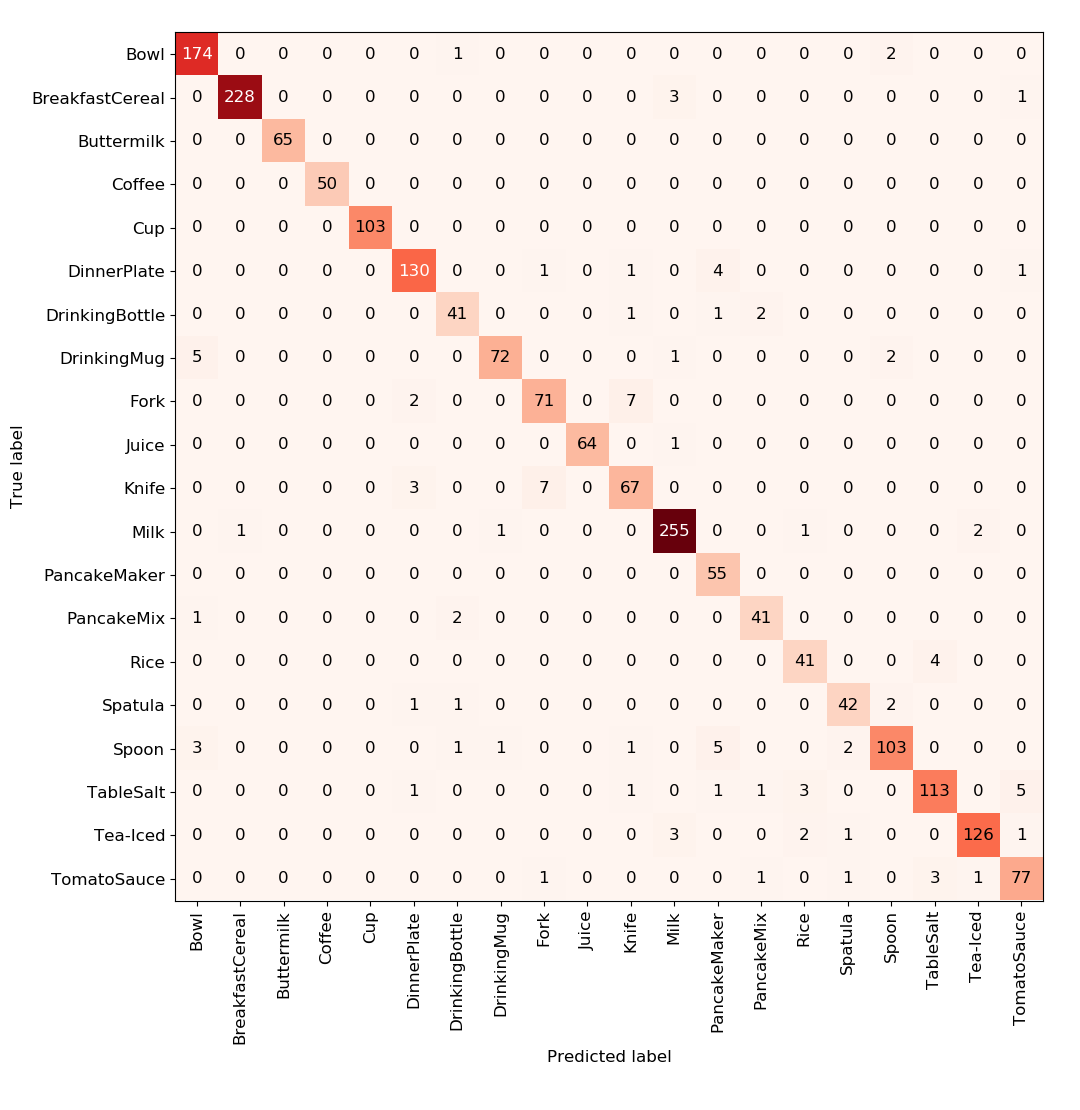
\includegraphics[scale=.315]{img/chapter6/UnrealGTClass.png}
\caption[Konfusionsmatrix des gesamten Unreal-Bilder Datensatzes mit Objektklassen als GT]{Die Konfusionsmatrix für die 10-fache Kreuzvalidierung der gesamten 570 Unreal-Bilder. Als \gls{gt} fungierten die Objektklassen.}
\label{fig:UnrealGTClass_confMatrix}
\end{figure}

Um dieses Modell zu evaluieren, wird 10-fache Kreuzvalidierung durchgeführt. Dabei wird der gesamte Datensatz, also alle 570 Bilder, in 10 Teilmengen aufgeteilt. Jedes Bild bleibt für den gesamten Prozess in seiner Teilmenge. Nun werden 9 Teilmengen als Trainingsdaten für ein \gls{mln} benutzt, während die übrige 10. Teilmenge zum Testen zur Verfügung steht. Dieser Vorgang wird 10 mal durchgeführt, sodass jede Teilmenge genau einmal zum Testen verwendet wurde. Die Ergebnisse der einzelnen Durchgänge können nun gemittelt werden. Dies verhindert die Überanpassung des Modells, also die Anpassung an die Trainingsdaten und damit einen Verlust der Generalität des Modells. \par

\subsection{Objektklassen}

\begin{table}
\centering
\small
\rowcolors{1}{}{lightgray}
\begin{tabularx}{\textwidth}{Xllll}
\textbf{Objekt}	& \textbf{\gls{accuracy}} & \textbf{\gls{precision}}	& \textbf{\gls{recall}}	& \textbf{\gls{f1score}} \\ \hline
Bowl & 0.99 & 0.95 & 0.98 & 0.97 \\  
BreakfastCereal & 1.0 & 1.0 & 0.98 & 0.99 \\  
Buttermilk & 1.0 & 1.0 & 1.0 & 1.0 \\  
Coffee & 1.0 & 1.0 & 1.0 & 1.0 \\  
Cup & 1.0 & 1.0 & 1.0 & 1.0 \\  
DinnerPlate & 0.99 & 0.95 & 0.95 & 0.95 \\  
DrinkingBottle & 1.0 & 0.89 & 0.91 & 0.9 \\  
DrinkingMug & 0.99 & 0.97 & 0.9 & 0.94 \\  
Fork & 0.99 & 0.89 & 0.89 & 0.89 \\  
Juice & 1.0 & 1.0 & 0.98 & 0.99 \\  
Knife & 0.99 & 0.86 & 0.87 & 0.86 \\  
Milk & 0.99 & 0.97 & 0.98 & 0.98 \\  
PancakeMaker & 0.99 & 0.83 & 1.0 & 0.91 \\  
PancakeMix & 1.0 & 0.91 & 0.93 & 0.92 \\  
Rice & 0.99 & 0.87 & 0.91 & 0.89 \\  
Spatula & 1.0 & 0.91 & 0.91 & 0.91 \\  
Spoon & 0.99 & 0.94 & 0.89 & 0.92 \\  
TableSalt & 0.99 & 0.94 & 0.9 & 0.92 \\  
Tea-Iced & 0.99 & 0.98 & 0.95 & 0.96 \\  
TomatoSauce & 0.99 & 0.91 & 0.92 & 0.91 \\  \hline
\textbf{Gesamt}		&	\textbf{0.95}   &	\textbf{0.95}  & \textbf{0.95}     &  \textbf{0.95}    \\
\end{tabularx}
\caption[Objektklassen-spezifische Kenngrößen des gesamten Unreal-Bilder Datensatzes]{Kenngrößen für die einzelnen Objekte aus der 10-fachen Kreuzvalidierung der gesamten Unreal-Bilder. Die Objektklassen sind die \gls{gt}.}
\label{tab:UnrealGTClass_metrics}
\end{table}

Die Ergebnisse der Kreuzvalidierung mit Objektklassen als \gls{gt} sind in Abbildung \ref{fig:UnrealGTClass_confMatrix} und Tabelle \ref{tab:UnrealGTClass_metrics} dargestellt. Insgesamt werden eine hohe \gls{accuracy} für alle Objektklassen als auch Werte über 90\% für \gls{precision}, \gls{recall} und \gls{f1score} erreicht. Einzig das Besteck und der Reis schneiden etwas schlechter ab. Bei dem Besteck war dies erwartet, da \textit{Knifes}, \textit{Forks} und \textit{Spoons} kleiner  als viele andere Objekte und damit visuelle Eigenschaften schwieriger auszumachen sind. Im Gegensatz zu den Ergebnissen der \glspl{klassifikator} ist eine deutliche Verbesserung zu erkennen. Vor allem werden keine Objekte gar nicht erkannt. Die bessere Klassifikationsrate war jedoch erwartet, da \glspl{mln} die Ergebnisse verschiedener Experten, die Annotatoren in \robosherlock, kombiniert und solche Ensembles, wie bereits zuvor dargelegt, zu besseren Ergebnissen kommen können. \newline
Um zu beweisen, dass dies auch hier der Fall ist, sind in den Abbildungen \ref{fig:singleEvidences} und \ref{fig:singleEvidencesGog} sind die Ergebnisse der 10-fachen Kreuzvalidierung mit nur jeweils einem Prädikat abgebildet. Dazu wurden die \glspl{mln} mit nur einem Prädikat von \robosherlock und dem $scene$-Prädikat trainiert und befragt. \newline
Es ist zu erkennen, dass bei Farbe, Form und Größe einige bestimmte Objekte präferiert werden. Die Anzahl er präferierten Objekte korrespondiert stark mit der Anzahl der möglichen Atome für jedes Prädikat. Es gibt zum Beispiel 10 Atome für Farbe, und in der Konfusionsmatrix 9-10 Objekte die regelmäßig klassifiziert werden. Bei der Form scheinen sich die 3 Atome auf je circa 2 Objekte zu verteilen: \textit{Fork}, \textit{Knife}, \textit{Spoon} für $small$, \textit{Tea-Iced} und \textit{DrinkingBottle} für $medium$ und \textit{PancakeMaker} und \textit{Tea-Iced} für $large$. Bei der Instanz fällt auf, dass vieles als \textit{Spoon} eingeordnet wird, während aber viele andere Objekt richtig zugeordnet sind. Diese Neigung war bei dem für die Instanz verantwortlichen \texttt{SVMAnnotator} in den vorherigen Experimenten interessanterweise nicht zu erkennen. Insgesamt scheinen sich die Fehler des \texttt{SVMAnnotators} im \gls{mln} nicht zu wiederholen, stattdessen tun sich andere auf. Der \texttt{GogglesAnnotator} hat sehr gute Ergebnisse auf texturierten oder beschrifteten Objekten. Insgesamt unterstützen diese Ergebnisse die Idee einer besseren Erkennung durch Ensembles, da jeder Annotator seine stärken und Schwächen aufweist, und erst durch die Zusammenführung der einzelnen Ergebnisse eine gute Klassifikationsrate erreicht wird.\par

\begin{figure}
\centering
	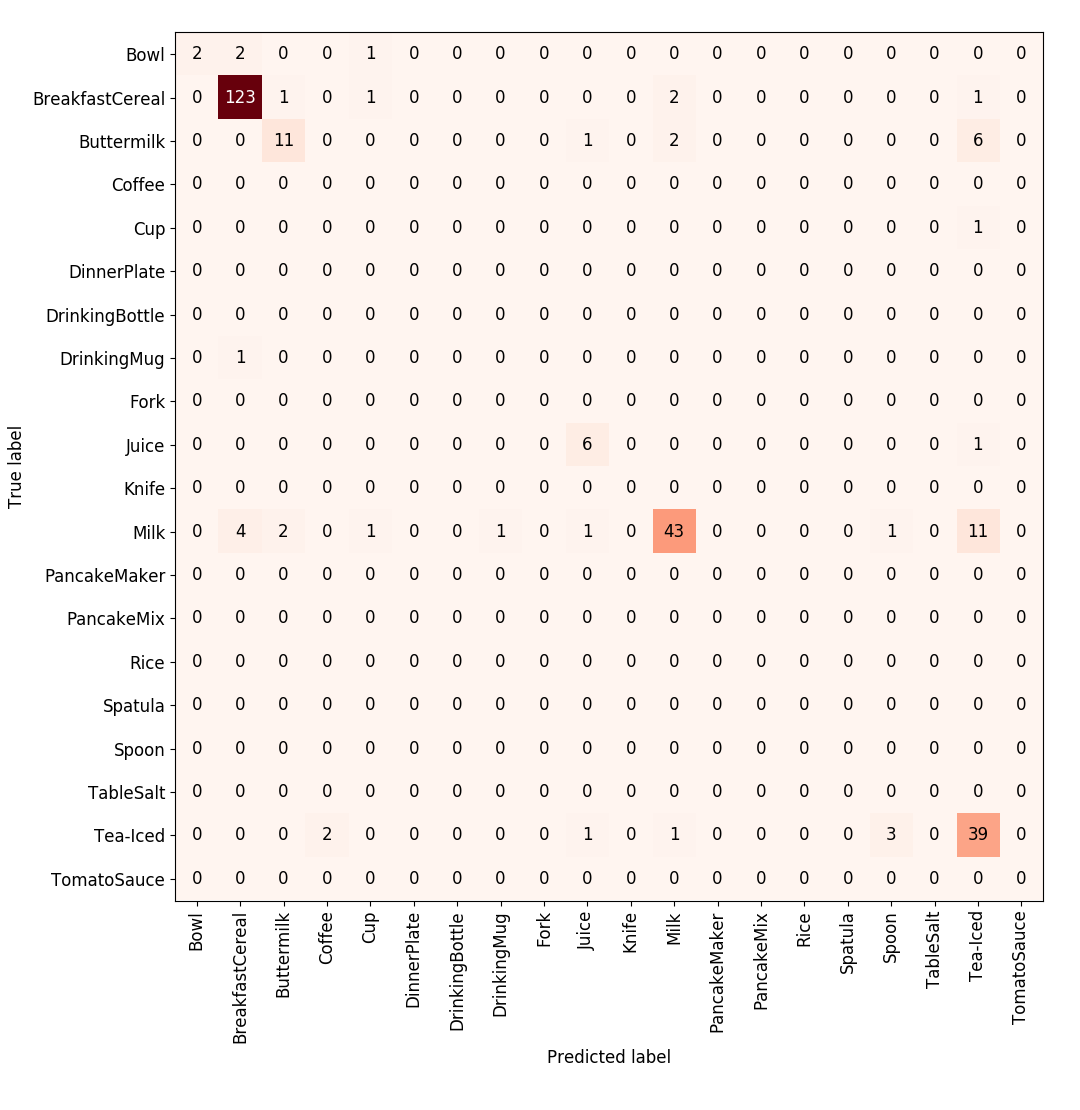
\includegraphics[scale=.27]{img/chapter6/UnrealGTClass_goggles.png}	
\caption[Konfusionsmatrix für die Klassifikation nur durch den \texttt{GogglesAnnotator}]{Konfusionsmatrix für die 10-fache Kreuzvalidierung der Unreal-Bilder, wobei nur die \texttt{GogglesAnnotator} und $scene$-Prädikate zum Trainieren und Testen verwendet wurden.}
\label{fig:singleEvidencesGog}
\end{figure}

\begin{figure}
\centering
	\begin{subfigure}[b]{0.48\textwidth}
		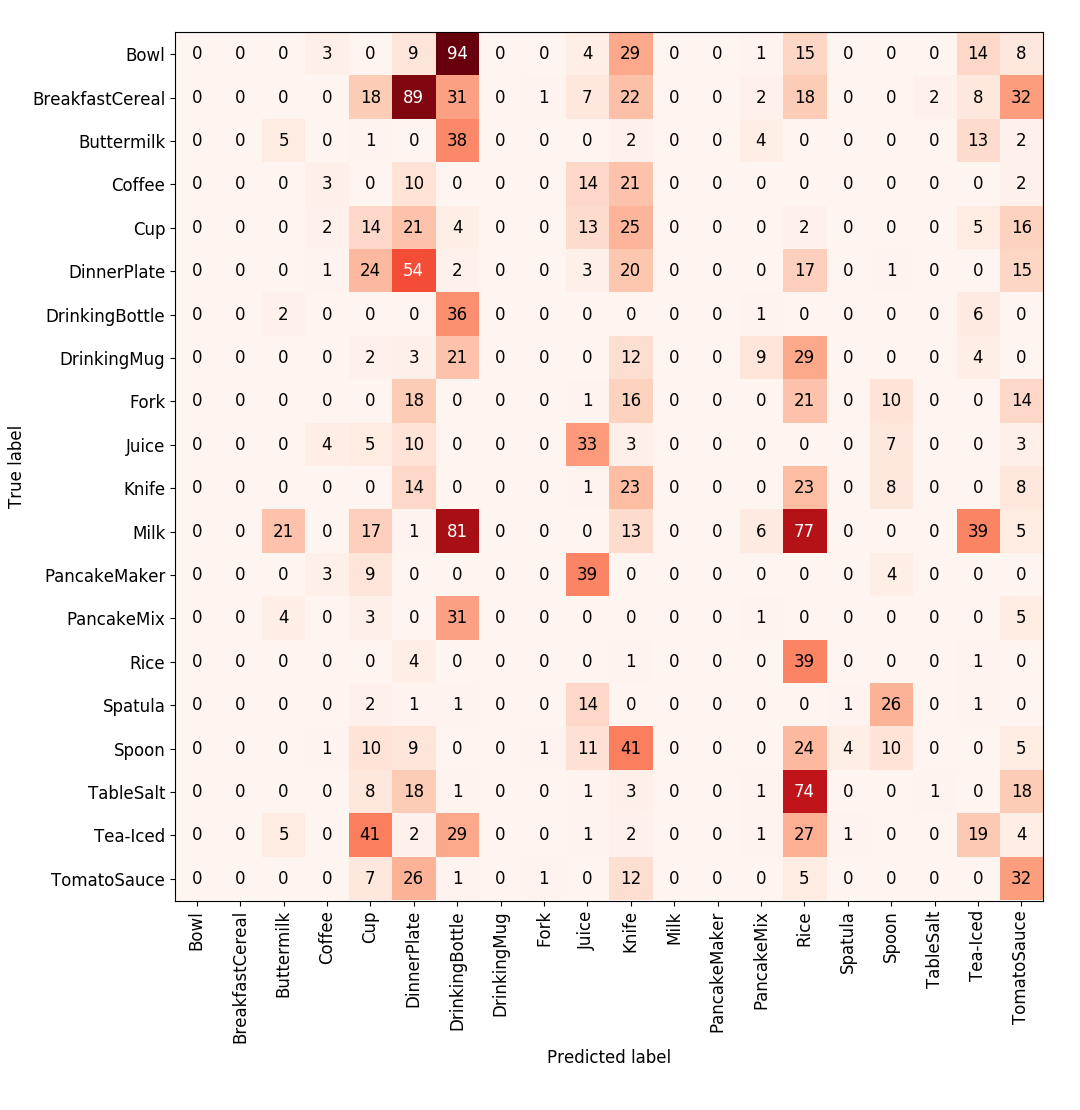
\includegraphics[scale=.27]{img/chapter6/UnrealGTClass_color.png}
		\subcaption{Farbe}
	\end{subfigure}
	\begin{subfigure}[b]{0.48\textwidth}
		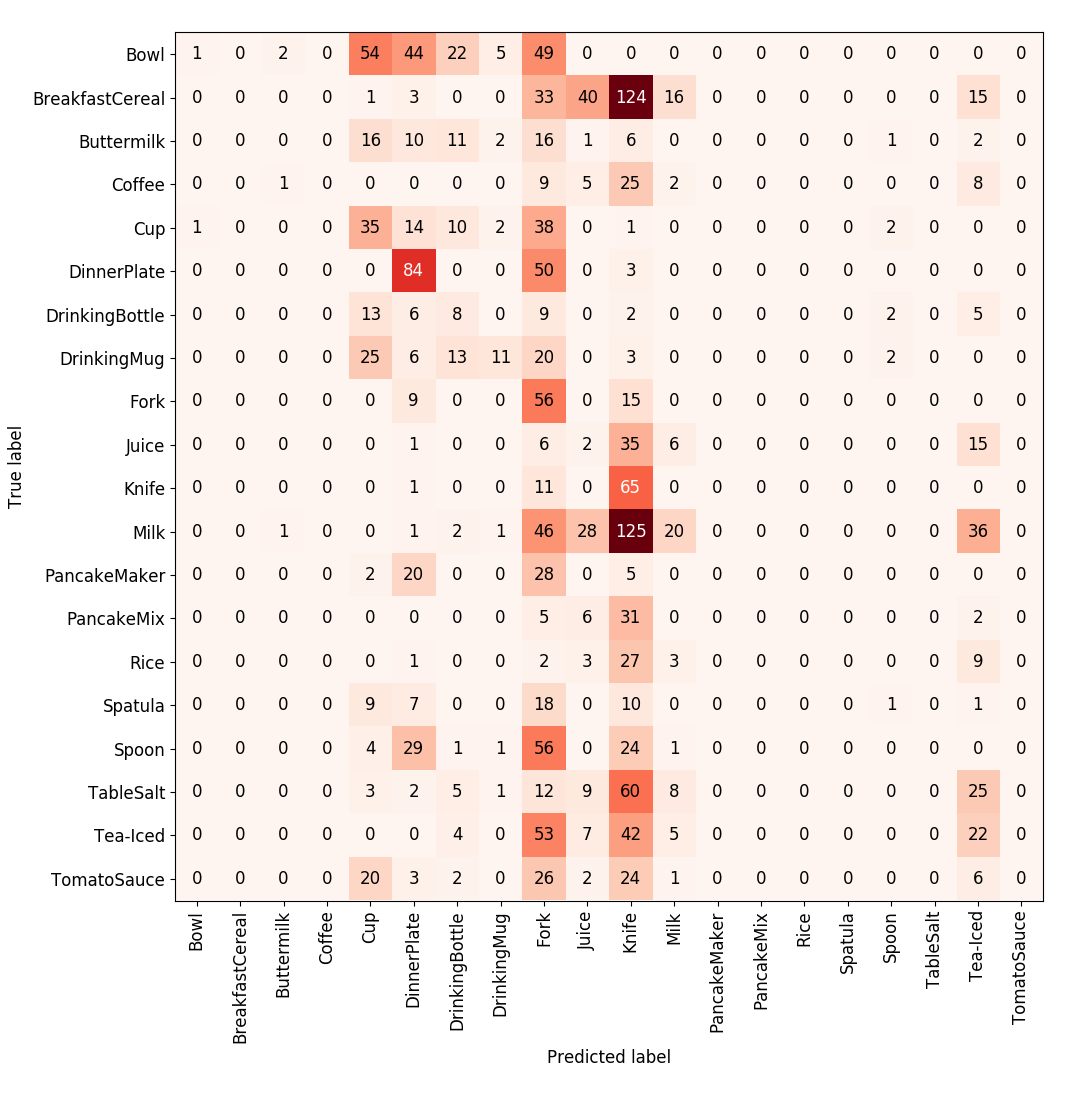
\includegraphics[scale=.27]{img/chapter6/UnrealGTClass_shape.png}	
		\subcaption{Form}
	\end{subfigure}
	\begin{subfigure}[b]{0.48\textwidth}
		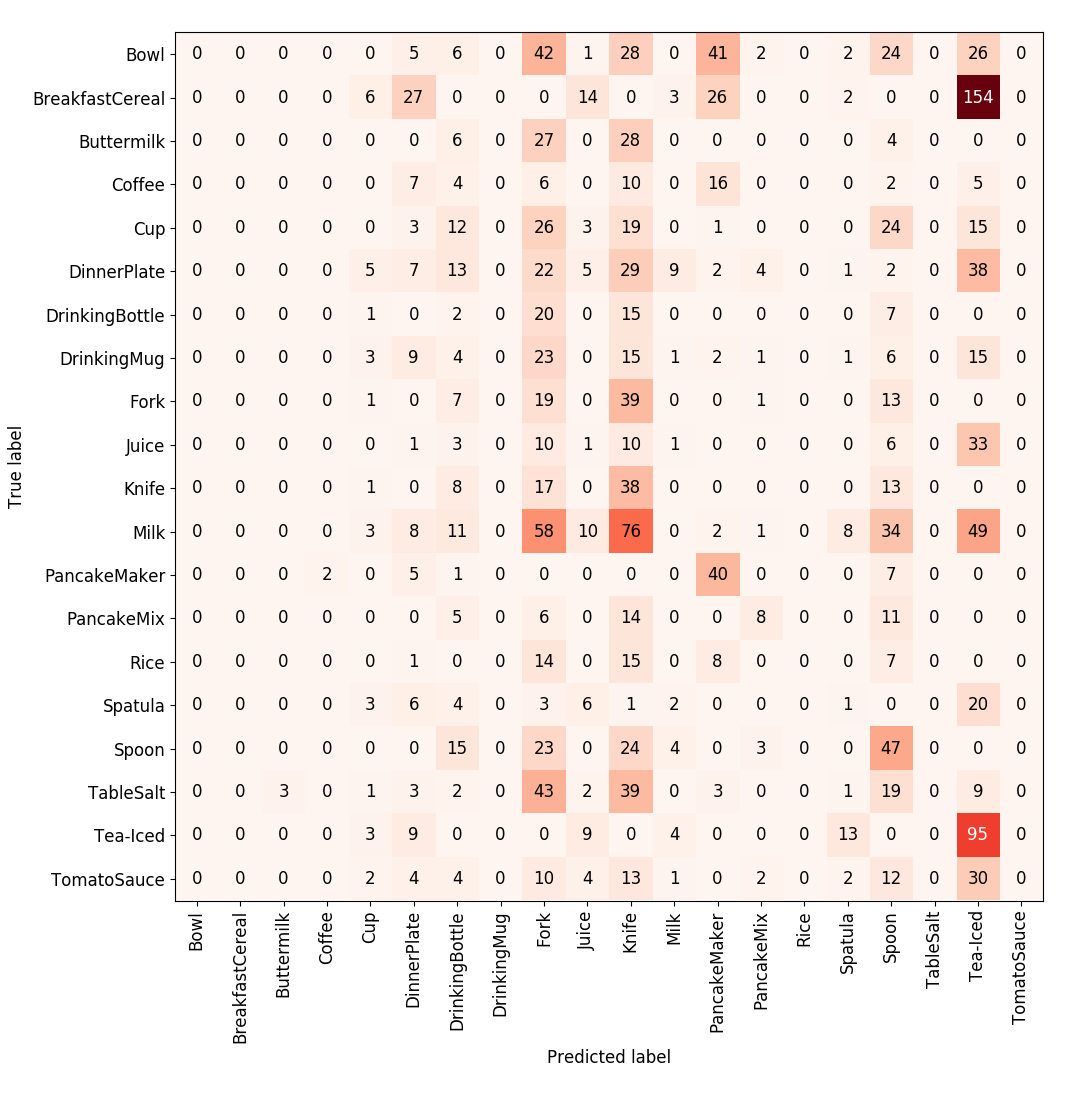
\includegraphics[scale=.27]{img/chapter6/UnrealGTClass_size.png}	
		\subcaption{Größe}
	\end{subfigure}
	\begin{subfigure}[b]{0.48\textwidth}
		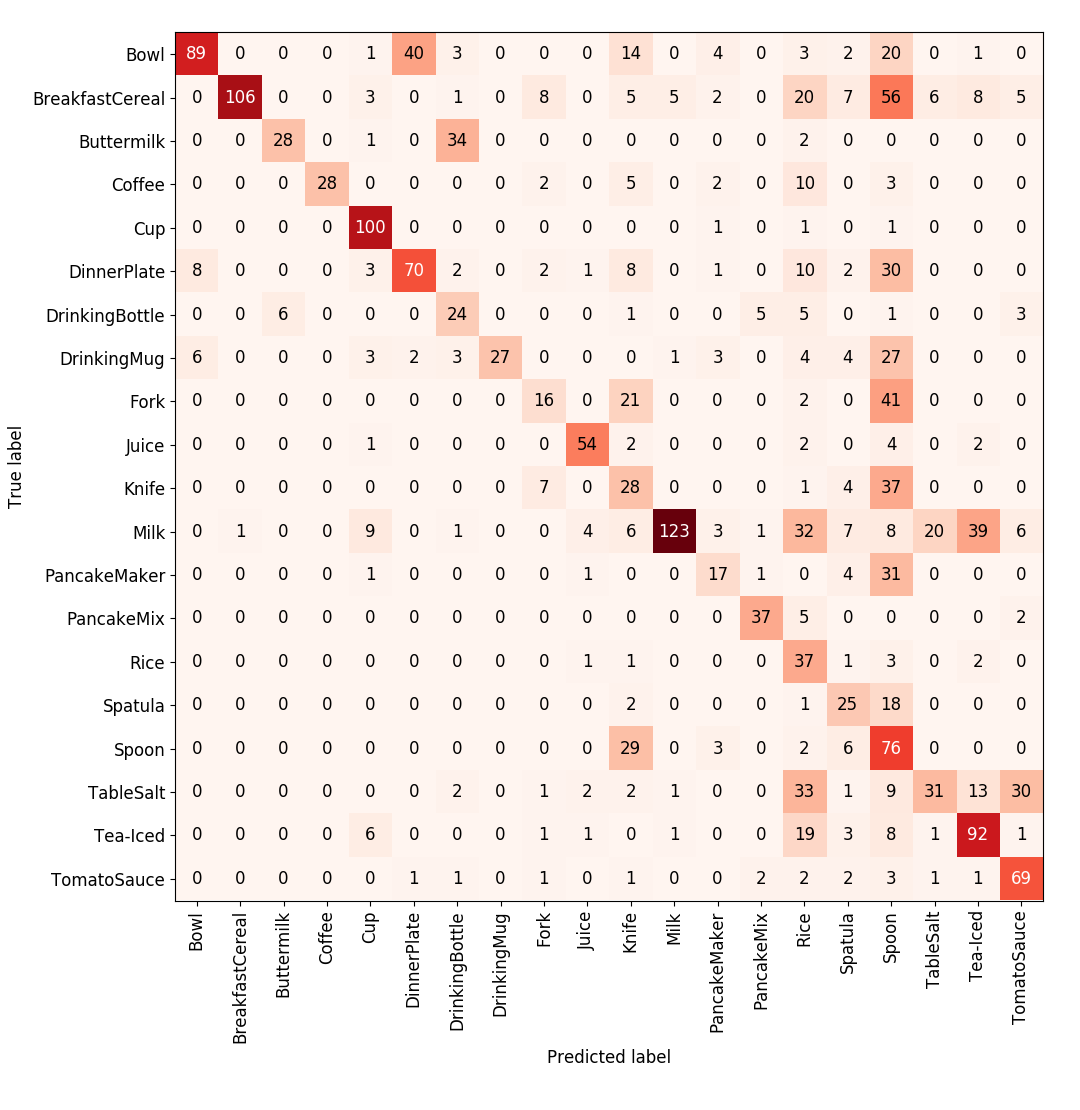
\includegraphics[scale=.27]{img/chapter6/UnrealGTClass_instance.png}	
		\subcaption{Instanz}
	\end{subfigure}
\caption[Konfusionsmatrizen für die Klassifikation mit nur einem Annotatoren Prädikat]{Konfusionsmatrizen der 10-fachen Kreuzvalidierung des gesamten Unreal-Bilder Satzes, wobei nur ein \robosherlock Prädikat (Form, Farbe, Größe, Instanz) und das $scene$-Prädikat zum Trainieren und Testen verwendet wurde.}
\label{fig:singleEvidences}
\end{figure}

\subsection{Instanznamen}

Die Ergebnisse der 10-fachen Kreuzvalidierung mit Instanznamen als \gls{gt} sind in Abbildung \ref{fig:UnrealGTInstance_confMatrix} und Tabelle \ref{tab:UnrealGTInstance_metrics} einzusehen. Wieder werden Werte über 90\% für fast alle Objekte erreicht. Ausnahmen bilden das rote Besteck, der \textit{SeverinPancakeMaker} und der \textit{LargeGreySpoon}. Letzterer wird häufig als besagter PancakeMaker eingestuft, während der PancakeMaker selber meistens durchaus korrekt klassifiziert wird (zu sehen am hohen \gls{recall} gegenüber der \gls{precision}). Das Selbe konnte für den \textit{SeverinPancakeMaker} und seine Klasse \textit{PancakeMaker} auch schon bei der Klassifikation der Objektklassen beobachtet werden. Bei den \glspl{klassifikator} verhielt es sich dagegen genau anderes herum. Zwei der roten Besteckteile, die \textit{RedPlasticFork} und das \textit{RedPlasticKnife}, liegen mit \gls{precision}, \gls{recall} und \gls{f1score} von unter 80\% deutlich unter dem Mittel der anderen Objekte und auch unter dem des anderen Bestecks. Denn selbst die blauen Gegenstücke, die \textit{BluePlasticFork} und das \textit{BluePlasticKnife}, erreichen Werte über 90\%.

\begin{figure}
\centering
	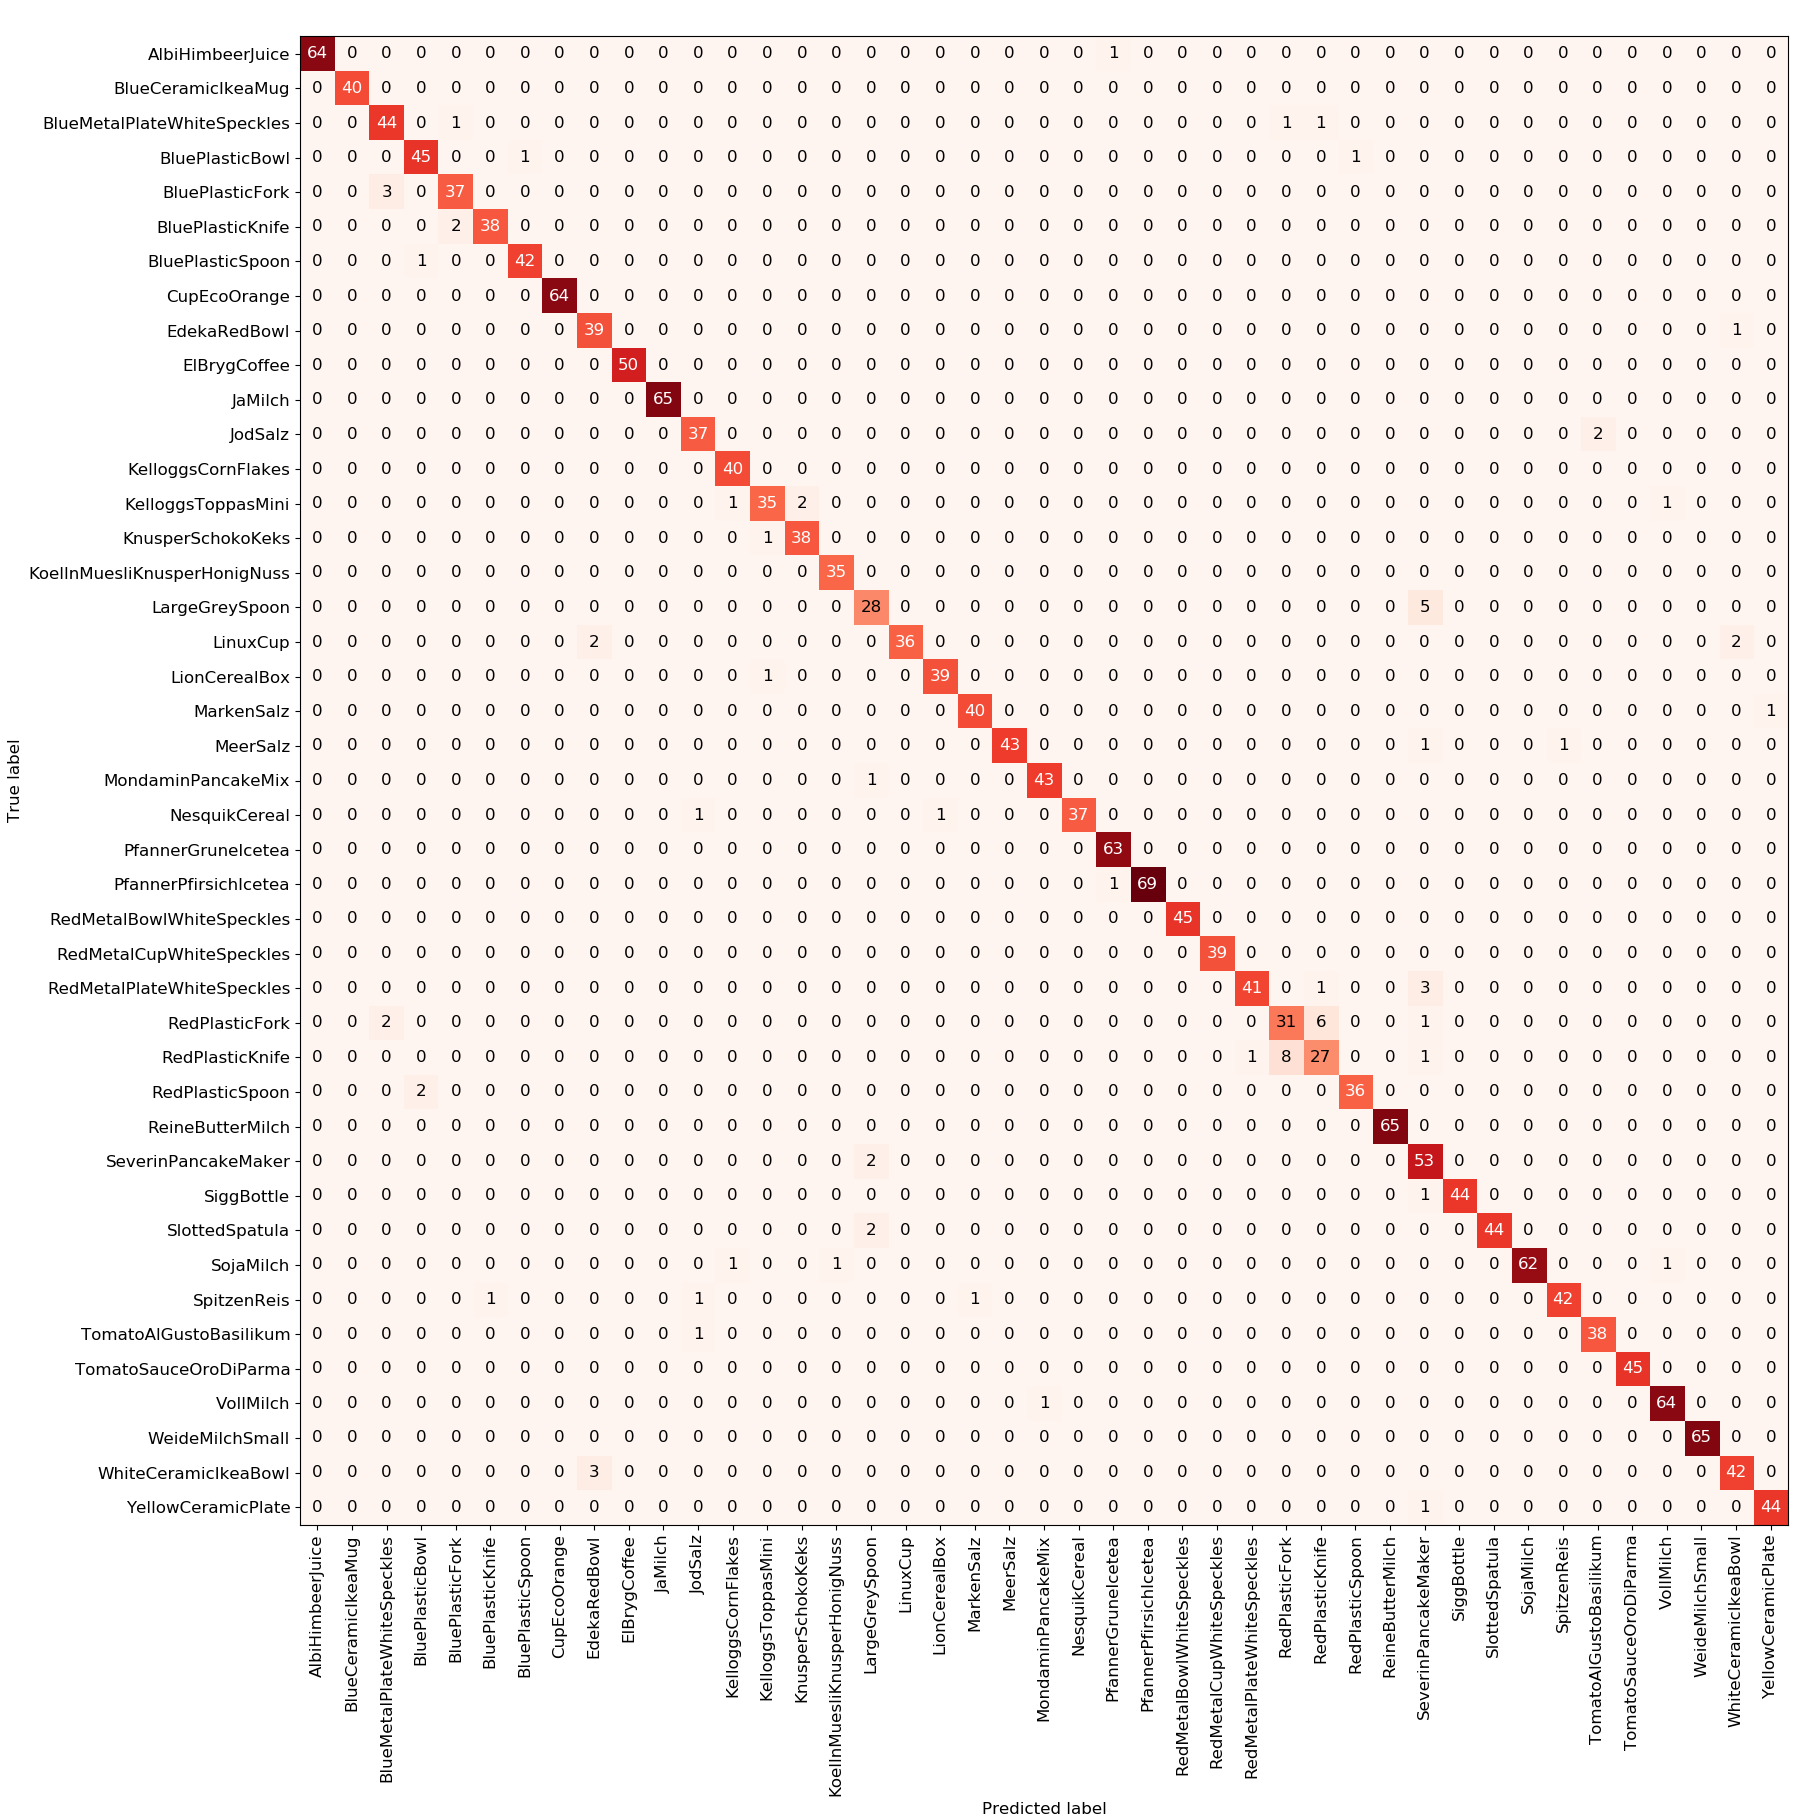
\includegraphics[scale=.292]{img/chapter6/UnrealGTInstance.png}
\caption[Konfusionsmatrix des gesamten Unreal-Bilder Datensatzes mit den Instanznamen als GT]{Die Konfusionsmatrix für die 10-fache Kreuzvalidierung der gesamten 570 Unreal-Bilder. Die \gls{gt} sind die Instanznamen.}
\label{fig:UnrealGTInstance_confMatrix}
\end{figure}

\begin{table}
\centering
\small
\rowcolors{1}{}{lightgray}
\begin{tabularx}{\textwidth}{Xllll}
\textbf{Objekt}	& \textbf{\gls{accuracy}} & \textbf{\gls{precision}}	& \textbf{\gls{recall}}	& \textbf{\gls{f1score}} \\ \hline
AlbiHimbeerJuice & 1.0 & 1.0 & 0.98 & 0.99 \\  
BlueCeramicIkeaMug & 1.0 & 1.0 & 1.0 & 1.0 \\  
BlueMetalPlateWhiteSpeckles & 1.0 & 0.9 & 0.94 & 0.92 \\  
BluePlasticBowl & 1.0 & 0.94 & 0.96 & 0.95 \\  
BluePlasticFork & 1.0 & 0.93 & 0.93 & 0.93 \\  
BluePlasticKnife & 1.0 & 0.97 & 0.95 & 0.96 \\  
BluePlasticSpoon & 1.0 & 0.98 & 0.98 & 0.98 \\  
CupEcoOrange & 1.0 & 1.0 & 1.0 & 1.0 \\  
EdekaRedBowl & 1.0 & 0.89 & 0.97 & 0.93 \\  
ElBrygCoffee & 1.0 & 1.0 & 1.0 & 1.0 \\  
JaMilch & 1.0 & 1.0 & 1.0 & 1.0 \\  
JodSalz & 1.0 & 0.93 & 0.95 & 0.94 \\  
KelloggsCornFlakes & 1.0 & 0.95 & 1.0 & 0.98 \\  
KelloggsToppasMini & 1.0 & 0.95 & 0.9 & 0.92 \\  
KnusperSchokoKeks & 1.0 & 0.95 & 0.97 & 0.96 \\  
KoellnMuesliKnusperHonigNuss & 1.0 & 0.97 & 1.0 & 0.99 \\  
LargeGreySpoon & 0.99 & 0.85 & 0.85 & 0.85 \\  
LinuxCup & 1.0 & 1.0 & 0.9 & 0.95 \\  
LionCerealBox & 1.0 & 0.97 & 0.97 & 0.97 \\  
MarkenSalz & 1.0 & 0.98 & 0.98 & 0.98 \\  
MeerSalz & 1.0 & 1.0 & 0.96 & 0.98 \\  
MondaminPancakeMix & 1.0 & 0.98 & 0.98 & 0.98 \\  
NesquikCereal & 1.0 & 1.0 & 0.95 & 0.97 \\  
PfannerGruneIcetea & 1.0 & 0.97 & 1.0 & 0.98 \\  
PfannerPfirsichIcetea & 1.0 & 1.0 & 0.99 & 0.99 \\  
RedMetalBowlWhiteSpeckles & 1.0 & 1.0 & 1.0 & 1.0 \\  
RedMetalCupWhiteSpeckles & 1.0 & 1.0 & 1.0 & 1.0 \\  
RedMetalPlateWhiteSpeckles & 1.0 & 0.98 & 0.91 & 0.94 \\  
RedPlasticFork & 0.99 & 0.78 & 0.78 & 0.78 \\  
RedPlasticKnife & 0.99 & 0.77 & 0.73 & 0.75 \\  
RedPlasticSpoon & 1.0 & 0.97 & 0.95 & 0.96 \\  
ReineButterMilch & 1.0 & 1.0 & 1.0 & 1.0 \\  
SeverinPancakeMaker & 0.99 & 0.8 & 0.96 & 0.88 \\  
SiggBottle & 1.0 & 1.0 & 0.98 & 0.99 \\  
SlottedSpatula & 1.0 & 1.0 & 0.96 & 0.98 \\  
SojaMilch & 1.0 & 1.0 & 0.95 & 0.98 \\  
SpitzenReis & 1.0 & 0.98 & 0.93 & 0.95 \\  
TomatoAlGustoBasilikum & 1.0 & 0.95 & 0.97 & 0.96 \\  
TomatoSauceOroDiParma & 1.0 & 1.0 & 1.0 & 1.0 \\  
VollMilch & 1.0 & 0.97 & 0.98 & 0.98 \\  
WeideMilchSmall & 1.0 & 1.0 & 1.0 & 1.0 \\  
WhiteCeramicIkeaBowl & 1.0 & 0.93 & 0.93 & 0.93 \\  
YellowCeramicPlate & 1.0 & 0.98 & 0.98 & 0.98 \\    \hline
\textbf{Gesamt}		&	\textbf{0.96}   &	\textbf{0.96}  & \textbf{0.96}     &  \textbf{0.96}     \\
\end{tabularx}
\caption[Objektinstanzen-spezifische Kenngrößen des gesamten Unreal-Bilder Datensatzes]{Kenngrößen für die einzelnen Objekte aus der 10-fachen Kreuzvalidierung der gesamten Unreal-Bilder .Die \gls{gt} sind die Instanznamen.}
\label{tab:UnrealGTInstance_metrics}
\end{table}

\begin{figure}
\centering
	\includegraphics[scale=.315]{img/chapter6/UnrealRealGTClass.png}
\caption[Konfusionsmatrix der Objektklassen Klassifikation mit Unreal-Trainingsset und realem Testset]{Die Konfusionsmatrix für die Klassifikation aller realen Bilder durch ein \gls{mln}, das mit allen Unreal-Bildern trainiert wurde. Als \gls{gt} wurden die Objektklassen verwendet.}
\label{fig:UnrealRealGTClass_confMatrix}
\end{figure}  

\section{Reale Bilder als Testdaten}

Im folgenden Experiment wird ein \gls{mln} mit den Unreal-Bildern trainiert und mit den realen Bildern getestet. Die Unreal-Bilder wurden wie zuvor von der in Kapitel \ref{sec:analysisengine} beschriebenen \gls{ae} annotiert. Die realen Bilder ebenfalls, allerdings ohne den \texttt{UnrealGTAnnotator} zu verwenden, da dieser nur für Bilder aus der \unreal geeignet ist und echte Bilder keine Asset-Namen zur Bestimmung der \gls{gt} aufweisen. Dementsprechend wurde die \gls{gt} manuell annotiert. Damit die Atome für den \texttt{GogglesAnnotator} in beiden Datensätzen übereinstimmen, wurde das Clustering mit den Annotationen aus beiden Datensätzen durchgeführt. Die Deklaration des \gls{mln} und Parameter beim Lernen und Anfragen sind unverändert gegenüber dem vorherigen Experiment. \par

\subsection{Objektklassen}

Bei der Klassifizierung der Objektklassen (Abbildung \ref{fig:UnrealRealGTClass_confMatrix}, Tabelle \ref{tab:UnrealRealGTClass_metrics}) ist die \gls{accuracy} für alle Klassen über 90\%, während auch die Werte für \gls{precision}, \gls{recall} und \gls{f1score} in den meisten Fällen mit über 70\% relativ hoch ausfallen. Ausnahmen bilden wie erwartet das Besteck, aber auch \textit{DrinkingBottle}, \textit{PancakeMix} und \textit{PancakeMaker} und der \textit{Rice}. Interessanterweise schneiden \textit{Spoons} und \textit{Forks} dabei deutlich besser ab als \textit{Knives}. Besonders schlecht schneidet auch der \textit{Spatula} ab, was auch schon bei den \glspl{klassifikator} aufgefallen war. Da die 10-fache Kreuzvalidierung, bei der nur Unreal-Bilder verwendet wurden, dieses Problem nicht zeigte, kann angenommen werden, dass das 3D-Modell keine gute Repräsentation des echten Objektes darstellt. Dass die Performance bei \textit{Rice} so stark abfällt, ist interessant, da die Erkennungsrate für andere texturierte Objekte (\textit{BreakfastCereal}, \textit{Milk}, \textit{TableSalt}, \textit{Tea-Iced}, \textit{TomatoSauce}) nicht so stark abfällt. Der wahrscheinlich wegen seiner Form von den \glspl{klassifikator} noch gut erkannte \textit{PancakeMix}, scheint diesen Vorteil hier nicht ausspielen zu können, während das für \textit{Buttermilk} mit einer 100 prozentigen Klassifikationsrate nicht gilt. Für den \textit{PancakeMaker} scheint das Selbe zu gelten, wie für den \textit{Spatula}, da auch er schon bei den \glspl{klassifikator} eine Problemquelle darstellte. 

\begin{table}
\centering
\small
\rowcolors{1}{}{lightgray}
\begin{tabularx}{\textwidth}{Xllll}
\textbf{Objekt}	& \textbf{\gls{accuracy}} & \textbf{\gls{precision}}	& \textbf{\gls{recall}}	& \textbf{\gls{f1score}} \\ \hline
Bowl & 0.98 & 0.88 & 0.99 & 0.93 \\  
BreakfastCereal & 0.96 & 0.8 & 0.96 & 0.87 \\  
Buttermilk & 1.0 & 1.0 & 1.0 & 1.0 \\  
Coffee & 0.99 & 1.0 & 0.81 & 0.9 \\  
Cup & 0.99 & 0.97 & 0.92 & 0.95 \\  
DinnerPlate & 0.96 & 0.67 & 0.86 & 0.75 \\  
DrinkingBottle & 0.98 & 0.73 & 0.41 & 0.52 \\  
DrinkingMug & 1.0 & 0.95 & 0.88 & 0.91 \\  
Fork & 0.96 & 0.61 & 0.6 & 0.6 \\  
Juice & 0.99 & 1.0 & 0.74 & 0.85 \\  
Knife & 0.94 & 0.37 & 0.27 & 0.31 \\  
Milk & 0.96 & 0.99 & 0.77 & 0.86 \\  
PancakeMaker & 0.98 & 0.7 & 0.47 & 0.56 \\  
PancakeMix & 0.98 & 0.57 & 0.33 & 0.42 \\  
Rice & 0.97 & 0.35 & 0.5 & 0.41 \\  
Spatula & 0.95 & 0.16 & 0.25 & 0.2 \\  
Spoon & 0.95 & 0.75 & 0.66 & 0.7 \\  
TableSalt & 0.95 & 0.66 & 0.81 & 0.72 \\  
Tea-Iced & 0.96 & 0.75 & 0.72 & 0.73 \\  
TomatoSauce & 0.97 & 0.63 & 0.89 & 0.74 \\   \hline
\textbf{Gesamt}		&	\textbf{0.76}   &	\textbf{0.78}  & \textbf{0.76}     &  \textbf{0.76}    \\
\end{tabularx}
\caption[Objektklassen-spezifische Kenngrößen der Klassifikation mit Unreal-Trainingsset und realem Testset]{Kenngrößen für die einzelnen Objekte der Klassifikation der realen Bilder durch ein \gls{mln}, das mit allen Unreal-Bildern trainiert wurde. Als \gls{gt} wurden die Objektklassen verwendet.}
\label{tab:UnrealRealGTClass_metrics}
\end{table}

\subsection{Instanznamen}

Die Ergebnisse für die Klassifikation mit den Instanznamen als \gls{gt} sind in Abbildung \ref{fig:UnrealRealGTInstance_confMatrix} und Tabelle \ref{tab:UnrealRealGTInstance_metrics} zu finden. Im Gegensatz zur 10-fachen Kreuzvalidierung des gesamten Unreal-Bilder Satzes, steigert sich die Erkennungsrate gegenüber der Objektklassen nicht leicht, sondern verschlechtert sich. Als Probleme fallen mal wieder der \textit{SlottedSpatula} und der \textit{LargeGreySpoon} ins Auge, die wieder häufig verwechselt werden. Am schlechtesten schneidet die \textit{WhiteCermaicIkeaBowl} ab, die meistens für die \textit{BluePlasticBowl} gehalten wird, welche auch häufiger falsch klassifiziert wurde. Ähnliche Ergebnisse der beiden Schüsseln waren auch bei den \glspl{klassifikator} zu beobachten. Das kleine Besteck schneidet wie üblich nicht so gut ab. Während \textit{Spoons} allerdings in fast allen \gls{mln} Klassifikationen das am besten erkannte Besteck sind, bildeten sie bei den \glspl{klassifikator} noch das Schlusslicht. Ansonsten gibt es, die wie zuvor schon erwähnten Ungenauigkeiten bei ähnlich farbigen und/oder texturierten Objekten aus \textit{TableSalt}, \textit{Milk}, \textit{Tea-Iced}, \textit{BreakfastCereal} und \textit{PancakeMix}. \par

\begin{figure}
\centering
	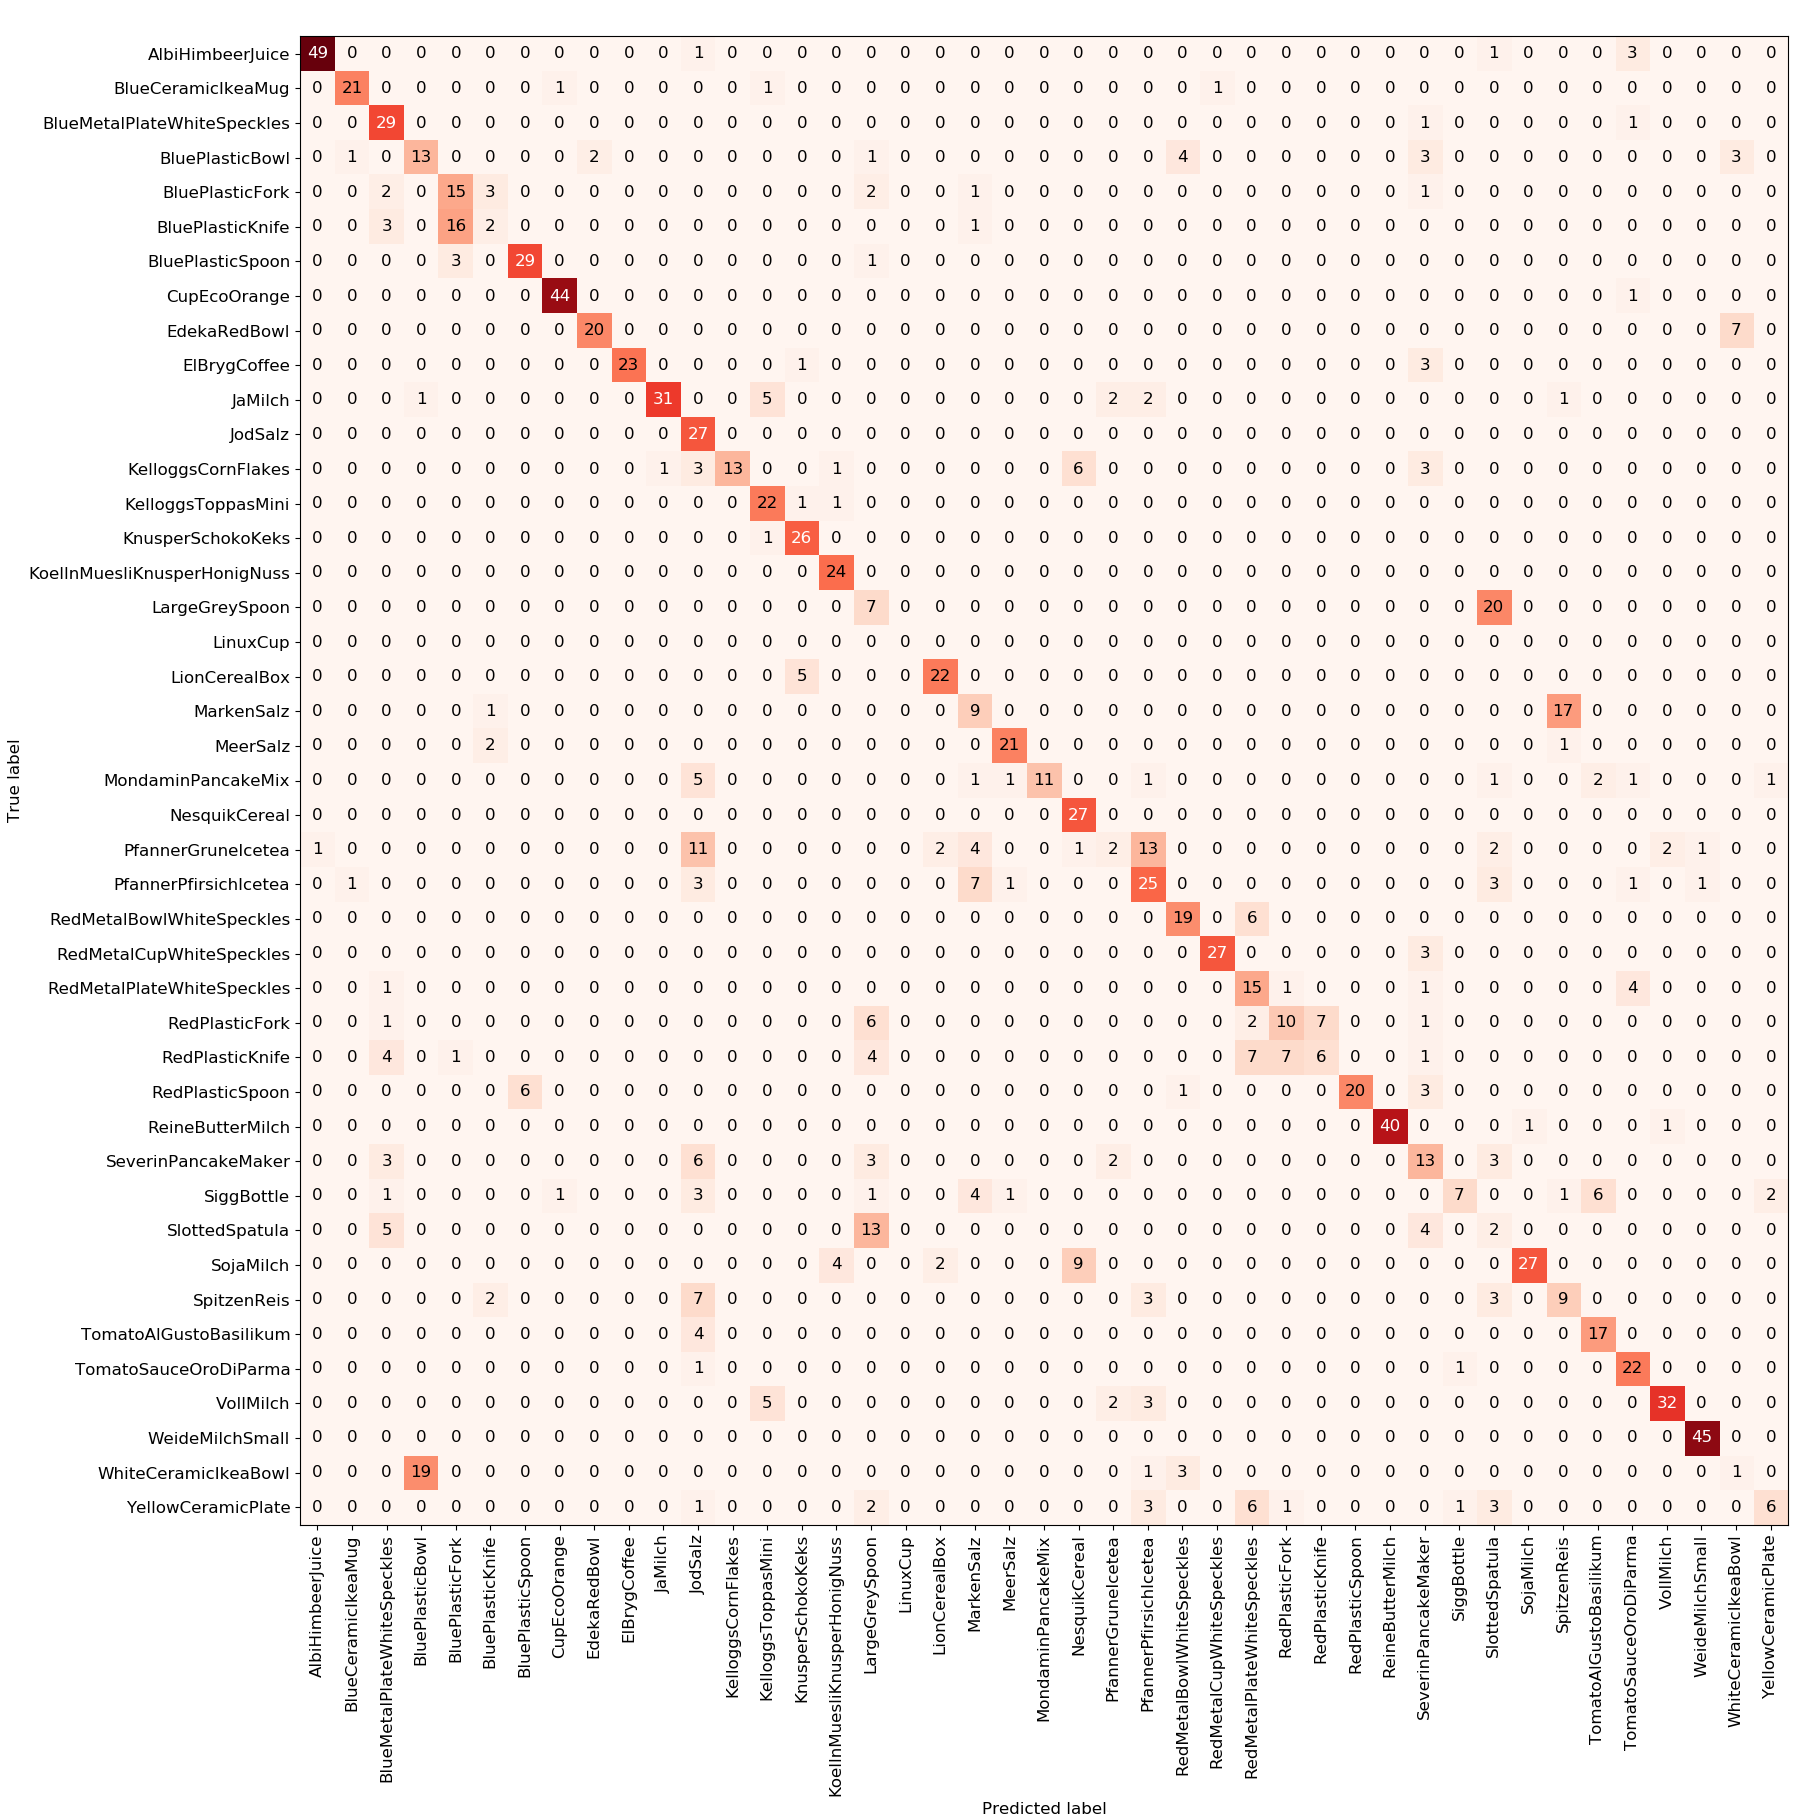
\includegraphics[scale=.292]{img/chapter6/UnrealRealGTInstance.png}
\caption[Konfusionsmatrix der Objektinstanzen Klassifikation mit Unreal-Trainingsset und realem Testset]{Die Konfusionsmatrix für die Klassifikation aller realen Bilder durch ein \gls{mln}, das mit allen Unreal-Bildern trainiert wurde. Als \gls{gt} wurden die Objektinstanzen verwendet.}
\label{fig:UnrealRealGTInstance_confMatrix}
\end{figure} 

\begin{table}
\centering
\small
\rowcolors{1}{}{lightgray}
\begin{tabularx}{\textwidth}{Xllll}
\textbf{Objekt}	& \textbf{\gls{accuracy}} & \textbf{\gls{precision}}	& \textbf{\gls{recall}}	& \textbf{\gls{f1score}} \\ \hline
AlbiHimbeerJuice & 0.99 & 0.98 & 0.91 & 0.94 \\  
BlueCeramicIkeaMug & 0.99 & 0.91 & 0.88 & 0.89 \\  
BlueMetalPlateWhiteSpeckles & 0.97 & 0.59 & 0.94 & 0.72 \\  
BluePlasticBowl & 0.96 & 0.39 & 0.48 & 0.43 \\  
BluePlasticFork & 0.97 & 0.43 & 0.63 & 0.51 \\  
BluePlasticKnife & 0.97 & 0.2 & 0.09 & 0.13 \\  
BluePlasticSpoon & 0.99 & 0.83 & 0.88 & 0.85 \\  
CupEcoOrange & 1.0 & 0.96 & 0.98 & 0.97 \\  
EdekaRedBowl & 0.99 & 0.91 & 0.74 & 0.82 \\  
ElBrygCoffee & 1.0 & 1.0 & 0.85 & 0.92 \\  
JaMilch & 0.99 & 0.97 & 0.74 & 0.84 \\  
JodSalz & 0.95 & 0.38 & 1.0 & 0.55 \\  
KelloggsCornFlakes & 0.98 & 1.0 & 0.48 & 0.65 \\  
KelloggsToppasMini & 0.98 & 0.65 & 0.92 & 0.76 \\  
KnusperSchokoKeks & 0.99 & 0.79 & 0.96 & 0.87 \\  
KoellnMuesliKnusperHonigNuss & 0.99 & 0.8 & 1.0 & 0.89 \\  
LargeGreySpoon & 0.94 & 0.17 & 0.26 & 0.21 \\  
LinuxCup & 1.0 & 0.0 & 0.0 & 0.0 \\  
LionCerealBox & 0.99 & 0.85 & 0.81 & 0.83 \\  
MarkenSalz & 0.96 & 0.33 & 0.33 & 0.33 \\  
MeerSalz & 0.99 & 0.88 & 0.88 & 0.88 \\  
MondaminPancakeMix & 0.98 & 1.0 & 0.46 & 0.63 \\  
NesquikCereal & 0.98 & 0.63 & 1.0 & 0.77 \\  
PfannerGruneIcetea & 0.95 & 0.25 & 0.05 & 0.09 \\  
PfannerPfirsichIcetea & 0.95 & 0.49 & 0.6 & 0.54 \\  
RedMetalBowlWhiteSpeckles & 0.98 & 0.7 & 0.76 & 0.73 \\  
RedMetalCupWhiteSpeckles & 1.0 & 0.96 & 0.9 & 0.93 \\  
RedMetalPlateWhiteSpeckles & 0.97 & 0.42 & 0.68 & 0.52 \\  
RedPlasticFork & 0.97 & 0.53 & 0.37 & 0.43 \\  
RedPlasticKnife & 0.96 & 0.46 & 0.2 & 0.28 \\  
RedPlasticSpoon & 0.99 & 1.0 & 0.67 & 0.8 \\  
ReineButterMilch & 1.0 & 1.0 & 0.95 & 0.98 \\  
SeverinPancakeMaker & 0.95 & 0.35 & 0.43 & 0.39 \\  
SiggBottle & 0.97 & 0.78 & 0.26 & 0.39 \\  
SlottedSpatula & 0.93 & 0.05 & 0.08 & 0.06 \\  
SojaMilch & 0.98 & 0.96 & 0.64 & 0.77 \\  
SpitzenReis & 0.96 & 0.31 & 0.38 & 0.34 \\  
TomatoAlGustoBasilikum & 0.99 & 0.68 & 0.81 & 0.74 \\  
TomatoSauceOroDiParma & 0.98 & 0.67 & 0.92 & 0.77 \\  
VollMilch & 0.98 & 0.91 & 0.76 & 0.83 \\  
WeideMilchSmall & 1.0 & 0.96 & 1.0 & 0.98 \\  
WhiteCeramicIkeaBowl & 0.96 & 0.09 & 0.04 & 0.06 \\  
YellowCeramicPlate & 0.98 & 0.67 & 0.26 & 0.38 \\     \hline
\textbf{Gesamt}		&	\textbf{0.66}   &	\textbf{0.69}  & \textbf{0.66}     &  \textbf{0.65}    \\
\end{tabularx}
\caption[Objektinstanzen-spezifische Kenngrößen der Klassifikation mit Unreal-Trainingsset und realem Testset]{Kenngrößen für die einzelnen Objekte der Klassifikation der realen Bilder durch ein \gls{mln}, das mit allen Unreal-Bildern trainiert wurde. Als \gls{gt} wurden die Objektinstanzen verwendet.}
\label{tab:UnrealRealGTInstance_metrics}
\end{table} 


\begin{table}
\centering
\rowcolors{1}{}{lightgray}
\begin{tabularx}{\textwidth}{Xlllll}
\textbf{Experiment}	&	\textbf{\gls{gt}}	& \textbf{\gls{accuracy}} & \textbf{\gls{precision}}	& \textbf{\gls{recall}}	& \textbf{\gls{f1score}} \\ \hline
RFAnnotator				&Klasse		&0.6	&0.67	&0.6	&0.57	\\
SVMAnnotator			&Klasse		&0.62	&0.7	&0.62	&0.57	\\
RFAnnotator				&Instanz	&0.6	&0.62	&0.6	&0.58	\\
SVMAnnotator			&Instanz	&0.66	&0.72	&0.66	&0.62	\\ \hline
Kreuzvalidierung		&Klasse		&0.95	&0.95	&0.95	&0.95	\\
Kreuzvalidierung		&Instanz	&0.96	&0.96	&0.96	&0.96	\\ \hline
Test mit realen Bildern	&Klasse		&0.76	&0.78	&0.76	&0.76	\\
Test mit realen Bildern	&Instanz	&0.66	&0.69	&0.66	&0.65	\\ \hline
Gemischtes Trainingsset	&Klasse		&0.9	&0.91	&0.9	&0.9	\\
Gemischtes Trainingsset	&Instanz	&0.88	&0.88	&0.88	&0.88	\\
\end{tabularx}
\caption[Übersicht der Kenngrößen der einzelnen Experimente]{Die Tabelle enthält die einzelnen Kenngrößen der Klassifikationen aus den jeweiligen Experimenten.}
\label{tab:classification_all}
\end{table}

%\begin{figure}
%\centering
%	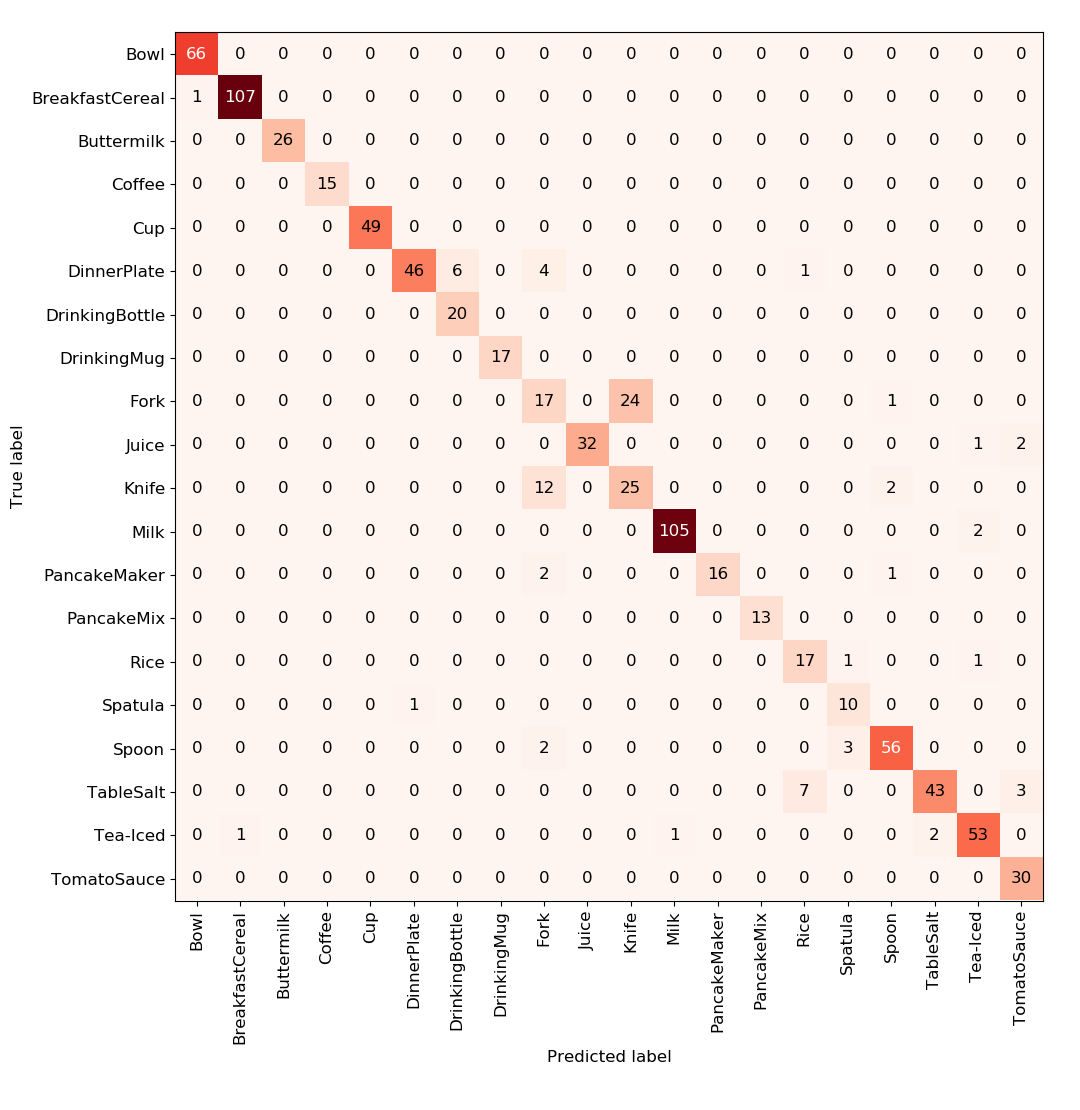
\includegraphics[scale=.315]{img/chapter6/UnrealRealMixedGTClass.png}
%\caption[Konfusionsmatrix der Objektklassen Klassifikation mit gemischtem Trainingsset und realem Testset]{Die Konfusionsmatrix für die \gls{mln}-Klassifikation der Klassen. Trainingsset sind alle Unreal-Bildern und ein drittel der realen Bilder, die restlichen.}
%\label{fig:UnrealRealMixedGTClass_confMatrix}
%\end{figure} 

\section{Ein gemischtes Trainigsset}
\label{unrealrealmixed}

Im letzten Experiment wurde ein Teil der realen Bilder zusätzlich zu den Unreal-Bildern zum Trainieren verwendet. Dazu wurde zufällig ein drittel der realen Bilder ausgewählt, womit insgesamt mit 684 Bildern trainiert wurde. Die restlichen 228 realen Bildern wurden wieder als Testdaten verwendet. \par

Die Konfusionsmatrizen sind in Abbildung \ref{fig:UnrealRealMixed_confMatrices} zu finden. Die Kenngrößen für die gesamte Klassifikation finden sich in Tabelle \ref{tab:classification_all}. Für beide \gls{gt}s hat sich die Performance gegenüber dem vorherigen Experiment gesteigert, sodass die beide bei allen Werten im Bereich um die 90\% liegen. Die meisten großen Fehlerquellen wurden durch das gemischte Trainingsset eliminiert. Nur die \textit{Knives} und \textit{Forks} bleiben wieder deutlich hinter dem Rest zurück. Allerdings haben sich die Werte für die Messer deutlich verbessert und liegen nun im Bereich der Gabeln und nicht wie zuvor deutlich darunter.  \par 

\begin{figure}
\centering
	\begin{subfigure}[b]{1\textwidth}
	\centering
	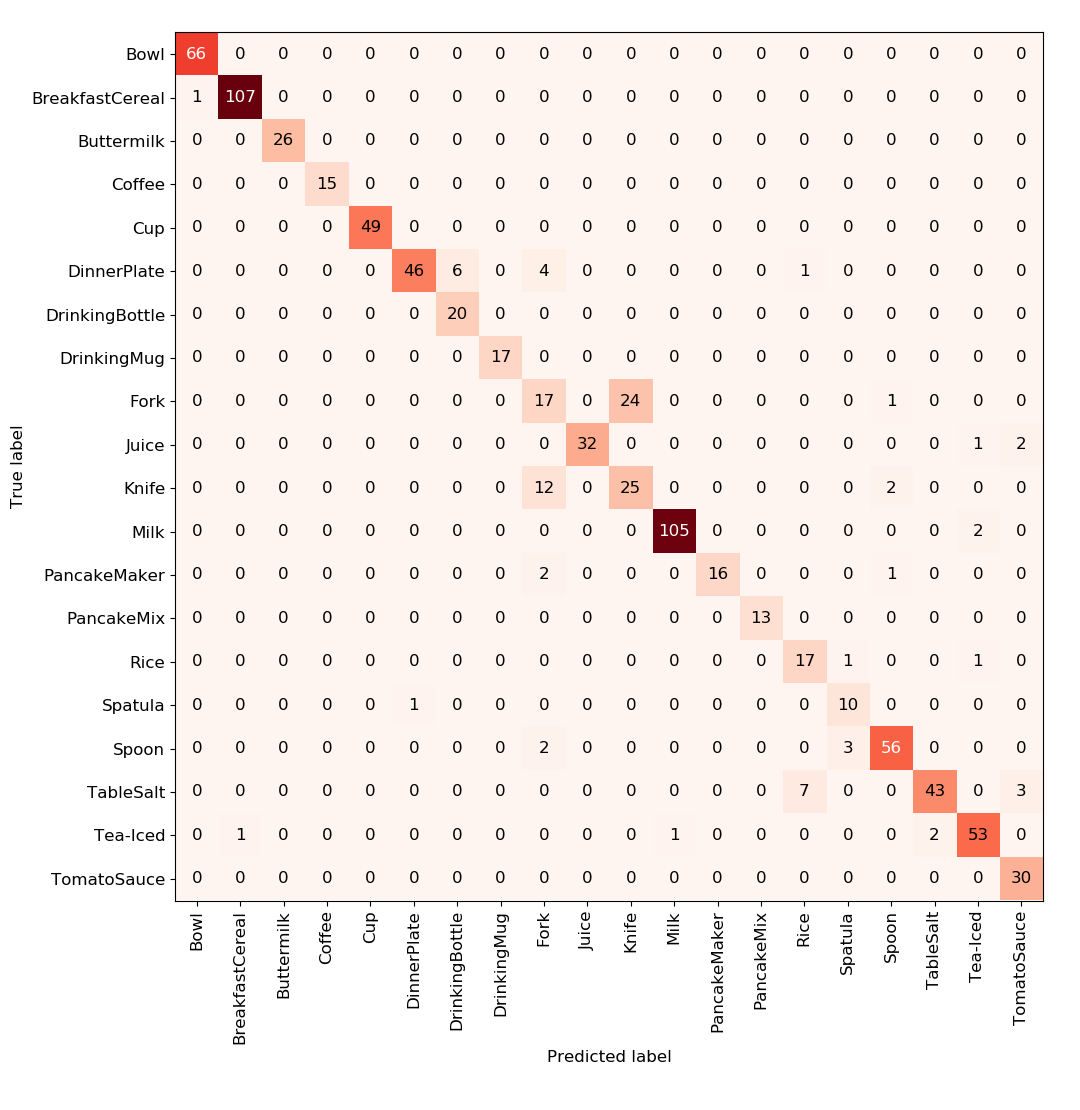
\includegraphics[scale=.29]{img/chapter6/UnrealRealMixedGTClass.png}
	\end{subfigure}
	\begin{subfigure}[b]{1\textwidth}
	\centering
	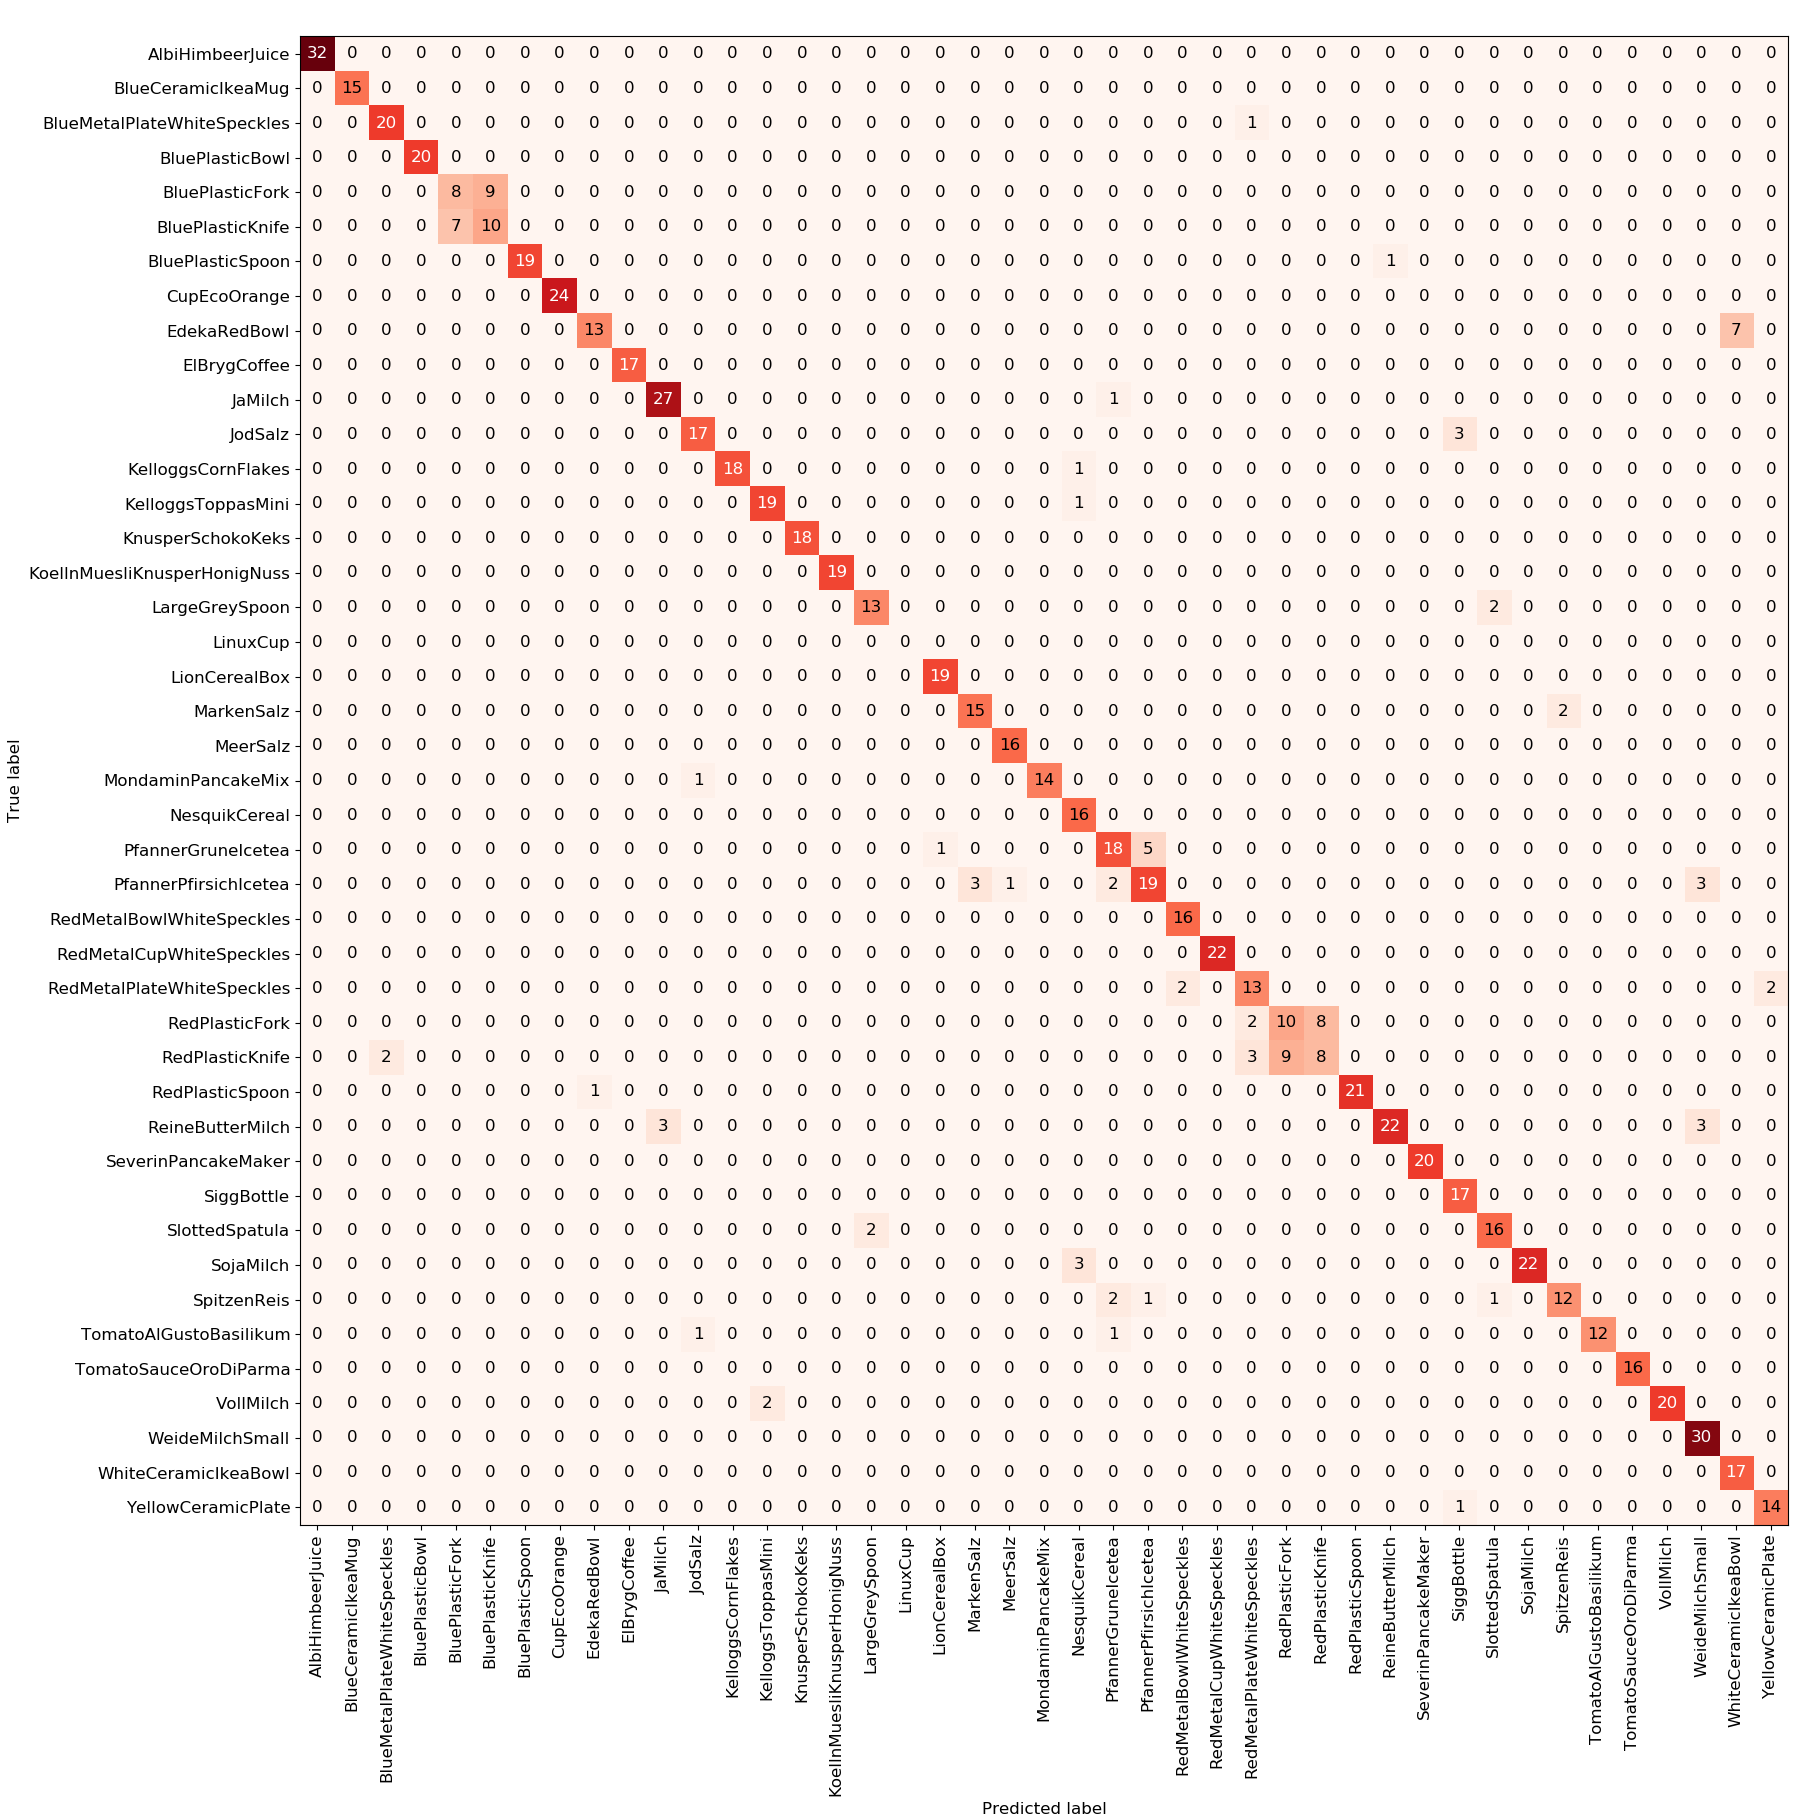
\includegraphics[scale=.29]{img/chapter6/UnrealRealMixedGTInstance.png}
	\end{subfigure}
\caption[Die Konfusionsmatrizen der Klassifikation mit gemischtem Trainingsset und realem Testset]{Die Konfusionsmatrizen für die \gls{mln}-Klassifikation mit gemischtem Trainingsset. Es besteht aus allen Unreal-Bildern und einem drittel der realen Bilder, die Restlichen bilden das Testset.}
\label{fig:UnrealRealMixed_confMatrices}
\end{figure}

%\begin{figure}
%\centering
%	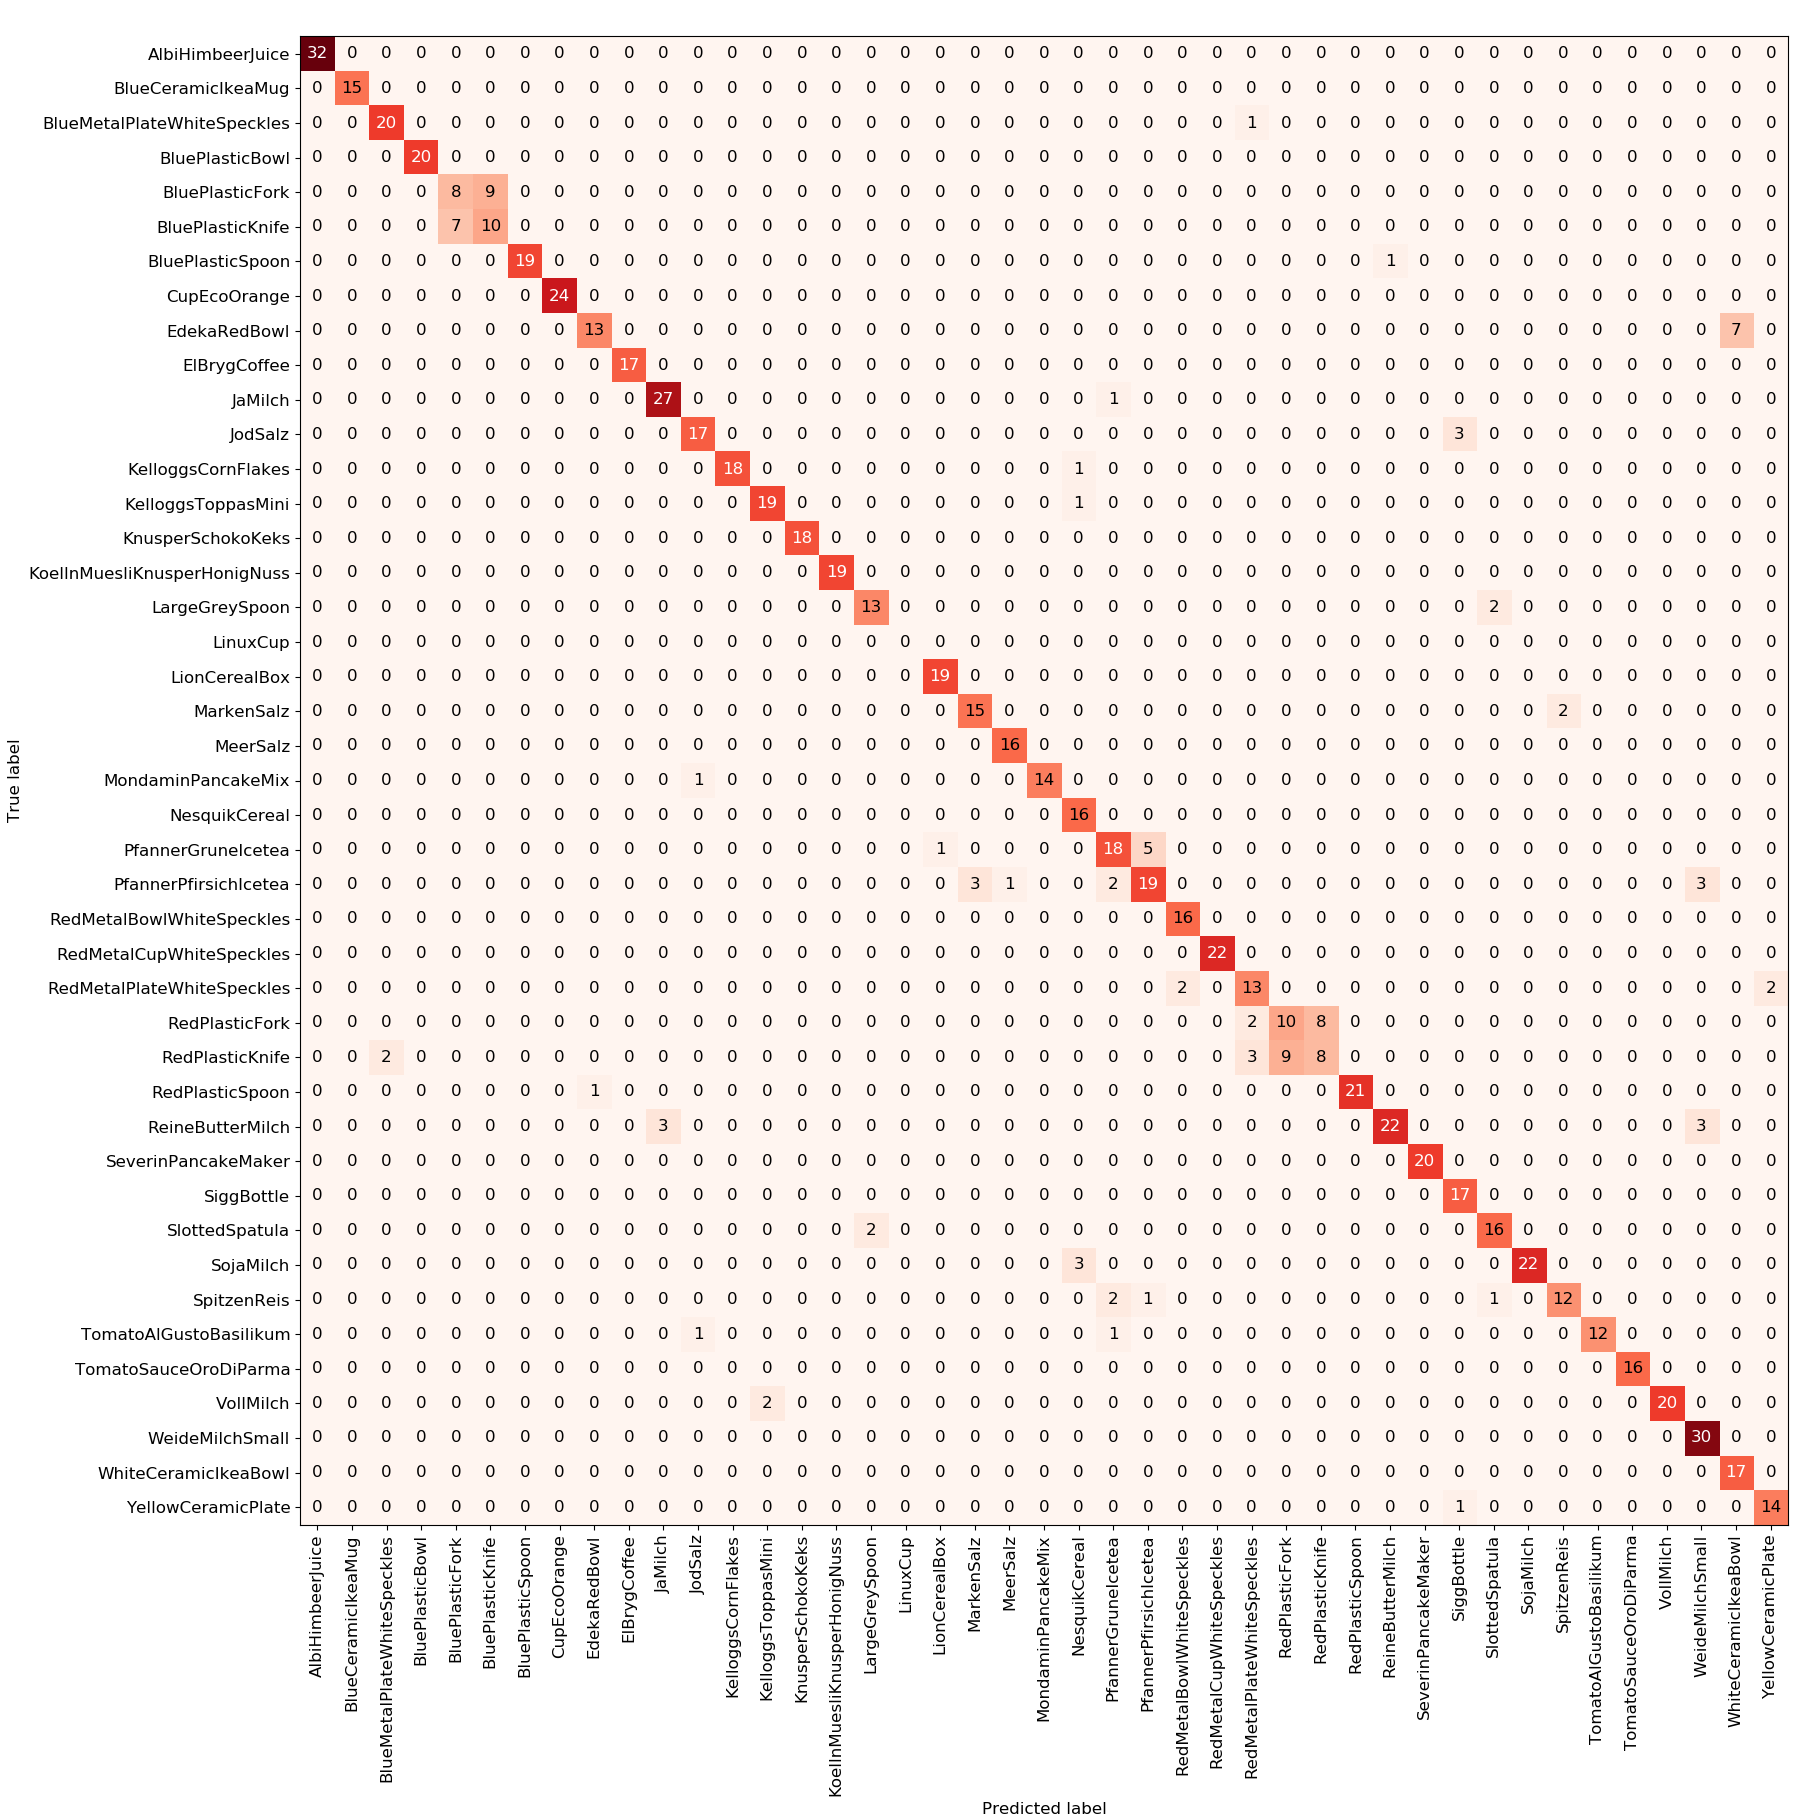
\includegraphics[scale=.292]{img/chapter6/UnrealRealMixedGTInstance.png}
%\caption[Konfusionsmatrix der Objektinstanzen Klassifikation mit gemischtem Trainingsset und realem Testset]{Die Konfusionsmatrix für die \gls{mln}-Klassifikation der Instanzen. Trainingsset sind alle Unreal-Bildern und ein drittel der realen Bilder, die restlichen bilden das Testset.}
%\label{fig:UnrealRealMixedGTInstance_confMatrix}
%\end{figure} 

%\begin{table}
%\centering
%\rowcolors{1}{}{lightgray}
%\begin{tabularx}{\textwidth}{Xllll}
%\textbf{Objekt}	& \textbf{\gls{accuracy}} & \textbf{\gls{precision}}	& \textbf{\gls{recall}}	& \textbf{\gls{f1score}} \\ \hline
%Bowl & 1.0 & 0.99 & 1.0 & 0.99 \\  
%BreakfastCereal & 1.0 & 0.99 & 0.99 & 0.99 \\  
%Buttermilk & 1.0 & 1.0 & 1.0 & 1.0 \\  
%Coffee & 1.0 & 1.0 & 1.0 & 1.0 \\  
%Cup & 1.0 & 1.0 & 1.0 & 1.0 \\  
%DinnerPlate & 0.98 & 0.98 & 0.81 & 0.88 \\  
%DrinkingBottle & 0.99 & 0.77 & 1.0 & 0.87 \\  
%DrinkingMug & 1.0 & 1.0 & 1.0 & 1.0 \\  
%Fork & 0.94 & 0.46 & 0.4 & 0.43 \\  
%Juice & 1.0 & 1.0 & 0.91 & 0.96 \\  
%Knife & 0.95 & 0.51 & 0.64 & 0.57 \\  
%Milk & 1.0 & 0.99 & 0.98 & 0.99 \\  
%PancakeMaker & 1.0 & 1.0 & 0.84 & 0.91 \\  
%PancakeMix & 1.0 & 1.0 & 1.0 & 1.0 \\  
%Rice & 0.99 & 0.68 & 0.89 & 0.77 \\  
%Spatula & 0.99 & 0.71 & 0.91 & 0.8 \\  
%Spoon & 0.99 & 0.93 & 0.92 & 0.93 \\  
%TableSalt & 0.98 & 0.96 & 0.81 & 0.88 \\  
%Tea-Iced & 0.99 & 0.93 & 0.93 & 0.93 \\  
%TomatoSauce & 0.99 & 0.86 & 1.0 & 0.92 \\  \hline
%\textbf{Gesamt}	&	\textbf{0.9}   &	\textbf{0.91}  & \textbf{0.9}   & \textbf{0.91} \\
%\end{tabularx}
%\caption[Objektklassen-spezifische Kenngrößen der Klassifikation mit gemischtem Trainingsset und realem Testset]{Kenngrößen für die einzelnen Objekte der Klassifikation durch ein \gls{mln}, das mit allen Unreal-Bildern und einem drittel der realen Bilder trainiert wurde. Getestet wurde mit den restlichen realen Bildern. Als \gls{gt} wurden die Objektklassen verwendet.}
%\label{tab:UnrealRealMixedGTClass_metrics}
%\end{table}

%\begin{table}
%\centering
%\small
%\rowcolors{1}{}{lightgray}
%\begin{tabularx}{\textwidth}{Xllll}
%\textbf{Objekt}	& \textbf{\gls{accuracy}} & \textbf{\gls{precision}}	& \textbf{\gls{recall}}	& \textbf{\gls{f1score}} \\ \hline
%AlbiHimbeerJuice & 1.0 & 1.0 & 1.0 & 1.0 \\  
%BlueCeramicIkeaMug & 1.0 & 1.0 & 1.0 & 1.0 \\  
%BlueMetalPlateWhiteSpeckles & 1.0 & 0.91 & 0.95 & 0.93 \\  
%BluePlasticBowl & 1.0 & 1.0 & 1.0 & 1.0 \\  
%BluePlasticFork & 0.98 & 0.53 & 0.47 & 0.5 \\  
%BluePlasticKnife & 0.98 & 0.53 & 0.59 & 0.56 \\  
%BluePlasticSpoon & 1.0 & 1.0 & 0.95 & 0.97 \\  
%CupEcoOrange & 1.0 & 1.0 & 1.0 & 1.0 \\  
%EdekaRedBowl & 0.99 & 0.93 & 0.65 & 0.76 \\  
%ElBrygCoffee & 1.0 & 1.0 & 1.0 & 1.0 \\  
%JaMilch & 0.99 & 0.9 & 0.96 & 0.93 \\  
%JodSalz & 0.99 & 0.89 & 0.85 & 0.87 \\  
%KelloggsCornFlakes & 1.0 & 1.0 & 0.95 & 0.97 \\  
%KelloggsToppasMini & 1.0 & 0.9 & 0.95 & 0.93 \\  
%KnusperSchokoKeks & 1.0 & 1.0 & 1.0 & 1.0 \\  
%KoellnMuesliKnusperHonigNuss & 1.0 & 1.0 & 1.0 & 1.0 \\  
%LargeGreySpoon & 0.99 & 0.87 & 0.87 & 0.87 \\  
%LinuxCup & 1.0 & 0.0 & 0.0 & 0.0 \\  
%LionCerealBox & 1.0 & 0.95 & 1.0 & 0.97 \\  
%MarkenSalz & 0.99 & 0.83 & 0.88 & 0.86 \\  
%MeerSalz & 1.0 & 0.94 & 1.0 & 0.97 \\  
%MondaminPancakeMix & 1.0 & 1.0 & 0.93 & 0.97 \\  
%NesquikCereal & 0.99 & 0.76 & 1.0 & 0.86 \\  
%PfannerGruneIcetea & 0.98 & 0.75 & 0.75 & 0.75 \\  
%PfannerPfirsichIcetea & 0.98 & 0.76 & 0.68 & 0.72 \\  
%RedMetalBowlWhiteSpeckles & 1.0 & 0.89 & 1.0 & 0.94 \\  
%RedMetalCupWhiteSpeckles & 1.0 & 1.0 & 1.0 & 1.0 \\  
%RedMetalPlateWhiteSpeckles & 0.99 & 0.68 & 0.76 & 0.72 \\  
%RedPlasticFork & 0.97 & 0.53 & 0.5 & 0.51 \\  
%RedPlasticKnife & 0.97 & 0.5 & 0.36 & 0.42 \\  
%RedPlasticSpoon & 1.0 & 1.0 & 0.95 & 0.98 \\  
%ReineButterMilch & 0.99 & 0.96 & 0.79 & 0.86 \\  
%SeverinPancakeMaker & 1.0 & 1.0 & 1.0 & 1.0 \\  
%SiggBottle & 0.99 & 0.81 & 1.0 & 0.89 \\  
%SlottedSpatula & 0.99 & 0.84 & 0.89 & 0.86 \\  
%SojaMilch & 1.0 & 1.0 & 0.88 & 0.94 \\  
%SpitzenReis & 0.99 & 0.86 & 0.75 & 0.8 \\  
%TomatoAlGustoBasilikum & 1.0 & 1.0 & 0.86 & 0.92 \\  
%TomatoSauceOroDiParma & 1.0 & 1.0 & 1.0 & 1.0 \\  
%VollMilch & 1.0 & 1.0 & 0.91 & 0.95 \\  
%WeideMilchSmall & 0.99 & 0.83 & 1.0 & 0.91 \\  
%WhiteCeramicIkeaBowl & 0.99 & 0.71 & 1.0 & 0.83 \\  
%YellowCeramicPlate & 1.0 & 0.88 & 0.93 & 0.9 \\   \hline
%\textbf{Gesamt}	& \textbf{0.88}   &	\textbf{0.88}  & \textbf{0.88} & \textbf{0.88}   \\
%\end{tabularx}
%\caption[Objektinstanzen-spezifische Kenngrößen der Klassifikation mit gemischtem Trainingsset und realem Testset]{Kenngrößen für die einzelnen Objekte der Klassifikation durch ein \gls{mln}, das mit allen Unreal-Bildern und einem drittel der realen Bilder trainiert wurde. Getestet wurde mit den restlichen realen Bildern. Als \gls{gt} wurden die Objektinstanzen verwendet.}
%\label{tab:UnrealRealMixedGTInstance_metrics}
%\end{table}

\graphicspath{{./images/}}      
\def\CHAPTERONE{./chapters/Chapter-1} 

\chapter{Fazit}
\label{chap:fazit}
%	\input{\CHAPTERONE /motivation}


\graphicspath{{./images/}}      
\def\CHAPTERONE{./chapters/Chapter-1} 

\chapter{Ausblick}
\label{chap:ausblick}
%	\input{\CHAPTERONE /motivation}


\pagenumbering{arabic}


\printglossary[style=altlist,title=Glossar]
\printglossary[type=\acronymtype,style=altlist,title=Akronyme]
%\printglossary[type=symbolslist,style=long]
%\printnomenclature
\clearpage{\pagestyle{empty}\cleardoublepage}
\cleardoublepage


%\setcounter{page}{1}
\pagenumbering{alph}


\addcontentsline{toc}{chapter}{Literaturverzeichnis}
\bibliography{bib}
%\cleardoublepage
%\addcontentsline{toc}{chapter}{Index}
%\printindex




\appendix
\chapter{Anhang}

USB-Stick mit:
\begin{itemize}
	\item \textbf{main.pdf}: dieses Dokument
	\item \textbf{bachelor\_experiments}: dieser Ordner enthält alle Ergebnisse der Experimente, sowie die eingesetzten \textit{python}-Skripte 
	\item \textbf{models}: dieser Ordner enthält die trainierten Modelle für den \texttt{RFAnnotator} und \texttt{SVMAnnotator}. \todo{wohin?}
	\item \textbf{Quellcode}: enthält den Quellcode der RSpawnBox und des UnrealGTAnnotators
\end{itemize}

\end{document}
